\documentclass{article}
\usepackage{graphicx}
\usepackage{geometry}
\usepackage{hyperref}
\usepackage{xcolor}
%%\usepackage{showframe}
\geometry{left=80pt,right=80pt,top=40pt,bottom=40pt}

\renewcommand*\contentsname{Table Des Matières}

\begin{document}
	\author{Thivagini SUGUMAR, Marine CONOR}
	\date{3 décembre 2023}
	
	\title{\underline{\textbf{M2 DataScale}}\\
		\bigskip
		\textbf{TP - Architectures Orientées Service}\\
		\bigskip
		Spécification du Service Web Composite : Evaluation de Demande de Prêt Immobilier
		\bigskip}
	
	\maketitle
	\newpage
	\tableofcontents
	\newpage
	\section{Notes sur le projet}
    Veuillez trouver les dernières versions du projet juste ici : 	
    \begin{itemize}
	 	\item \textcolor{blue}{\href{https://github.com/uvsq21704755/ProjetSOAP.git}{SOAP}} : \texttt{https://github.com/uvsq21704755/ProjetSOAP.git}
	 	\item \textcolor{blue}{\href{https://github.com/uvsq21704755/ProjetREST.git}{REST}} : \texttt{https://github.com/uvsq21704755/ProjetREST.git}
	 \end{itemize}
	\section{Contexte général du TP}
	Le service Web Composite d'Évaluation de Demande de Prêt Immobilier est conçu pour automatiser le processus d'évaluation des demandes de prêt immobilier en utilisant des services Web spécialisés. 
	\newline Il permet aux clients de soumettre des demandes de prêt immobilier exprimées en langage naturel. Le service intègre des composants d’extraction des informations métiers de texte de la demande, de vérification de solvabilité, d'évaluation de la propriété et de décision d'approbation pour fournir une évaluation complète et précise des demandes de prêt. 
	
	\section{Objectif}
	L'objectif de ce service est de fournir une interface unique pour les clients qui souhaitent demander un prêt immobilier. Le service coordonne les différents services Web nécessaires pour évaluer la demande du client, garantissant ainsi un processus fluide et automatisé.
	
	\section{Fonctionnement du système}
	\subsection{Architecture}
	Nous représentons l’architecture du fonctionnement du système par le diagramme suivant : 
	\\
	\\
		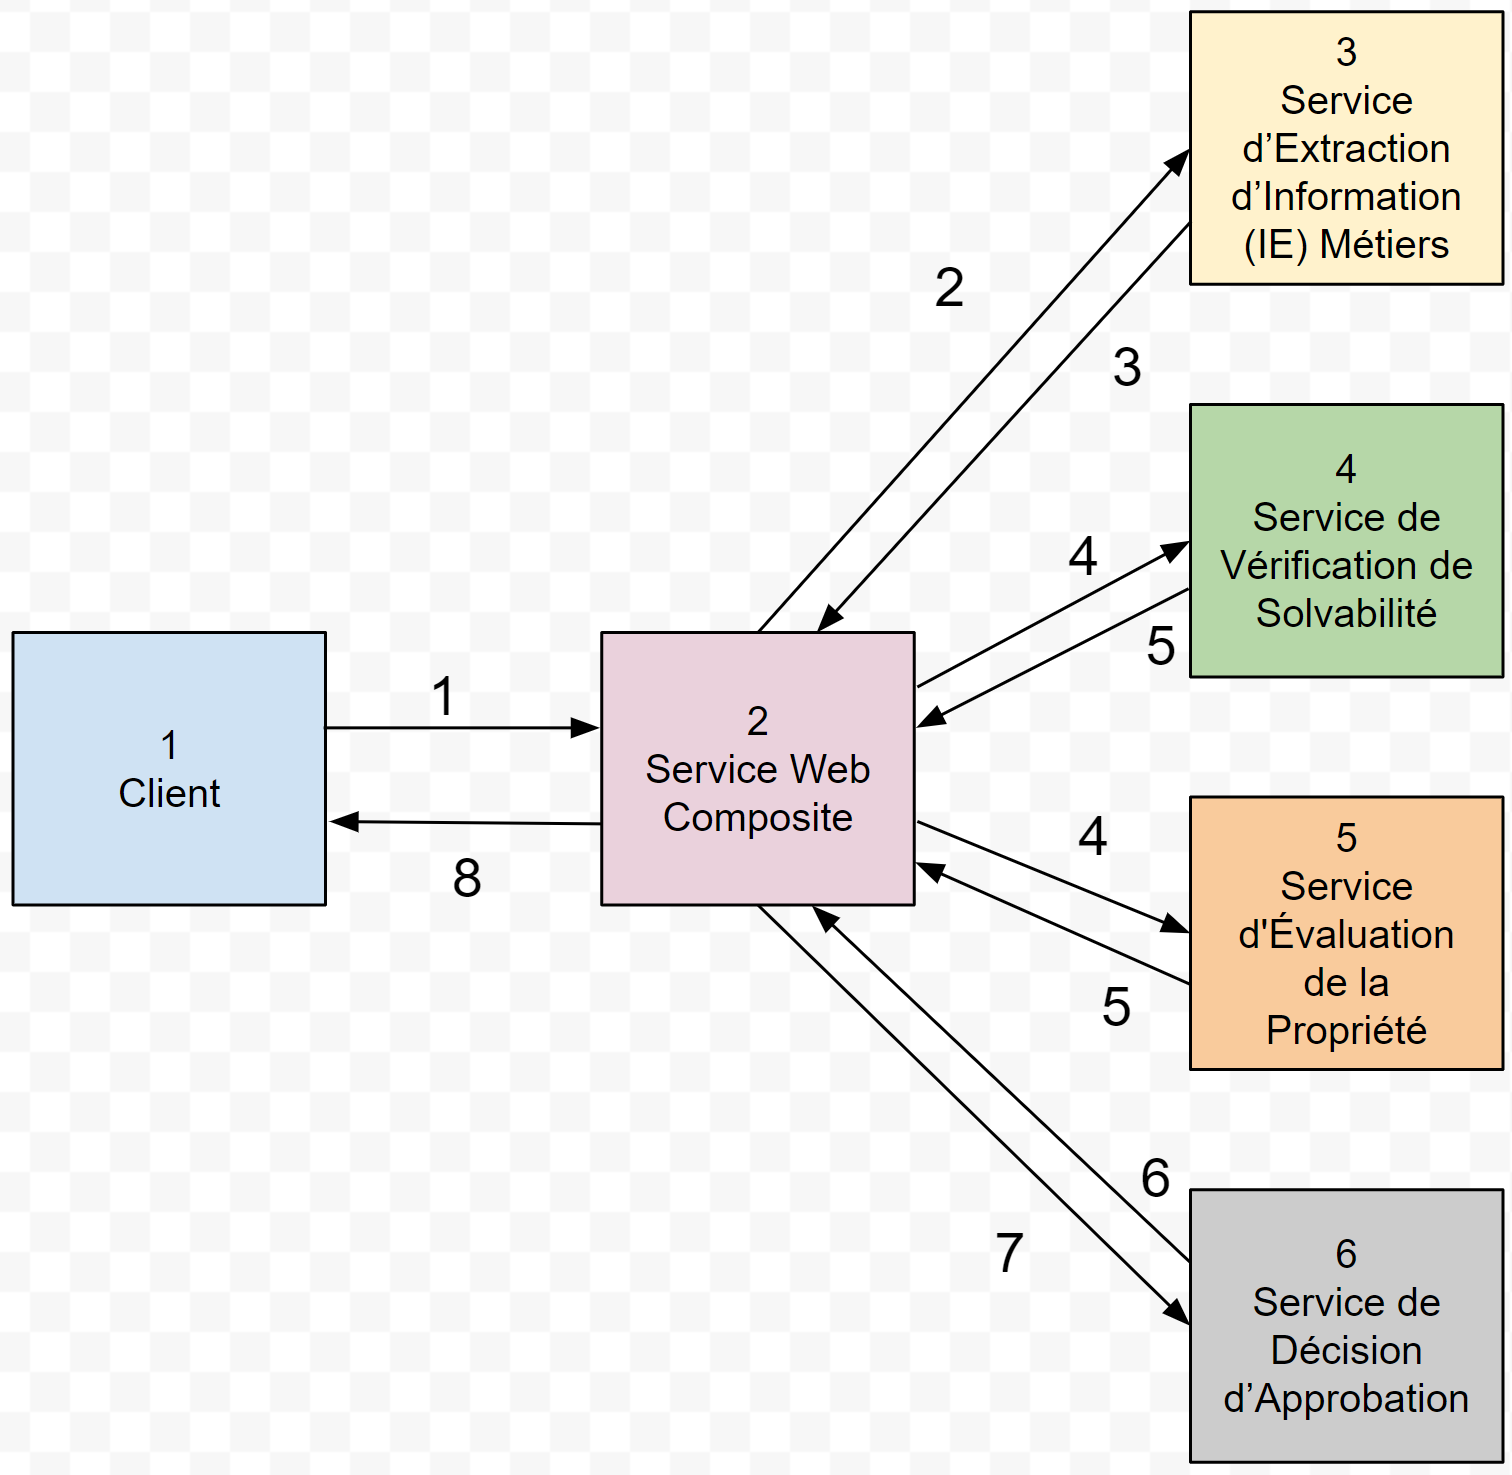
\includegraphics[width=240pt]{Images/4.1/architecture.png}
		
		\newpage
		
	\subsection{Étapes}
	  \begin{itemize}
	  	\item Sur l’interface, le client va effectuer une demande de prêt sur l'interface en soumettant un formulaire. Cette action va enclencher la création d'un fichier \texttt{txt} dans le répertoire \texttt{demandeTxt}
	  	
	  	\item Le service \textbf{Composite} va détecter l’arrivée du fichier \texttt{txt} dans le répertoire \texttt{demandeTxt} grâce à une routine qui se lance automatiquement. Ainsi le service composite va récupérer ce fichier \texttt{txt}
	  	
	  	\item Le service composite va effectuer une requête au service \textbf{Extraction} afin de récupérer le fichier WSDL
	  	
	  	\item Le service composite va alors transmettre le fichier \texttt{txt} au service d’\textbf{Extraction} via sa méthode web service encapsulé dans une enveloppe SOAP
	  	
	  	\item Le service d’\textbf{Extraction} va effectuer le prétraitement, identifier des entités et extraire les entités avec les expressions régulières. Cette extraction sera sauvegardée dans un fichier \texttt{XML} dans \texttt{demandeXML} sous le format : \texttt{numeroDossier.xml}
	  	
	  	\item Le service d’\textbf{Extraction} renvoie ce fichier \texttt{XML} obtenu au service \textbf{Composite}
	  	
	  	\item Le service \textbf{Composite} donne le fichier \texttt{XML} au service de \textbf{Vérification de Solvabilité}
	  	
	  	\item Le service de \textbf{Vérification de Solvabilité} va utiliser une fonction de scoring pour donner un score. Il ajoute les balises \texttt{<scoring></scoring>} et \texttt{<decisionScoring></decisionScoring>} dans le fichier \texttt{XML}
	  	
	  	\item Le service de \textbf{Vérification de Solvabilité} renvoie le fichier \texttt{XML} modifié au service \textbf{Composite}
	  
	  	\item Le service \textbf{Composite} donne le fichier \texttt{XML} modifié au service d'\textbf{Évaluation de la Propriété}
	  	
	  	\item Le service d'\textbf{Évaluation de la Propriété} va utiliser une fonction pour évaluer le marché immobilier afin de donner une moyenne et évaluer les normes légales et réglementaires du bâtiment. \\
	  	Il peut aussi décider de faire une visite virtuelle et une visite sur place. \\
	  	Il ajoute les balises : \\
	  	\texttt{<estimation\_valeur></estimation\_valeur>} et \\
	  	 \texttt{<decisionConformite></decisionConformite>}, si la décision est "Non admissible". \\
	  	Il ajoute également aussi une balise \texttt{<raisons></raisons>} dans le fichier \texttt{XML} donné en entrée
	  	
	  	\item Le service d'\textbf{Évaluation de la Propriété} renvoie le fichier \texttt{XML} modifié au service \textbf{Composite}
	  	
	  	\item Le service \textbf{Composite} donne le fichier \texttt{XML} modifié au service de \textbf{Décision d'Approbation}
	  	
	  	\item Le service de \textbf{Décision d’Approbation} va utiliser une fonction comparant les résultats et analyses précédents. Il va ensuite créer un nouveau fichier \texttt{txt} dans le dossier \texttt{reponseTxt} sous le format \texttt{numeroDossier.txt}
	  	
	  	\item Le service de \textbf{Décision d’Approbation} renvoie le fichier \texttt{txt} au service \textbf{Composite}
	  	
	  	\item Le client peut retrouver sa réponse sur l’interface en consultant les résultats
	  	
	  \end{itemize}
	
	\newpage
	
	\section{Identification des services}
		Les services identifiés sont les suivants : \\
		
		\begin{itemize}
			\item Le service \textbf{Composite} : \\
			
			Permet l’interaction entre le Client et les différents Services. Il s’occupe notamment de la réception de la demande, l’extraction d’information métier, la vérification de solvabilité, l’évaluation de la propriété et la décision d'approbation.
			
			\item Le service d’\textbf{Extraction} : \\
			
			Reçoit le texte de la demande de prêt soumise par le client, via le service \textbf{Composite}. \\
			Il s’occupe principalement du prétraitement, analyse, identification des entités et l’extraction de ces informations. De plus, il permet le stockage des informations extraites dans la base de données du service \textbf{Composite}
			
			\item Le service de \textbf{Vérification de Solvabilité} : \\
			
			Permet d'évaluer la capacité financière du client à rembourser le prêt. Il s’occupe donc de l’intégration des bureaux de crédit pour se connecter à leurs bureaux qui stockent l'historique financier des clients. Il récupère des informations telles que les dettes en cours, les paiements en retard et les antécédents de faillite pour évaluer la crédibilité du client. Ensuite, le service utilise des algorithmes de scoring de crédit pour attribuer un score au client en fonction de son historique financier. Ce score représente le niveau de risque associé à l'accord d'un prêt au client. Les clients avec des scores élevés ont une solvabilité plus élevée. Il analyse aussi les revenus et les dépenses mensuelles.
			
			\item Le service d'\textbf{Évaluation de la Propriété} :\\
			
			Permet d'estimer la valeur marchande de la propriété pour laquelle le prêt est demandé. Il peut utiliser des données immobilières, des expertises locales et des critères légaux pour effectuer cette évaluation. Il s’occupe donc d'analyser les données du marché immobilier, peut effectuer une inspection virtuelle de la propriété ou même des visites sur place et vérifier si la propriété est conforme aux normes légales et réglementaires en vigueur.
			
			\item Le service de \textbf{Décision d'Approbation} : \\
			
			Analyse les données recueillies lors des étapes précédentes (Vérification de Solvabilité et Évaluation de la Propriété) pour déterminer si le prêt immobilier peut être approuvé. Il s’occupe d’analyser les risques associés à l'accord du prêt, de comparer les données de la demande de prêt avec les politiques internes de l'institution financière pour évaluer la probabilité de défaut de paiement du client. En fonction des résultats, le service prend une décision d'approbation ou de refus du prêt puis communique celle-ci au service \textbf{Composite} (en indiquant les raisons de l'approbation ou du refus du prêt) qui va retourner cette réponse au client.
			
		\end{itemize}
	
	\newpage
	\section{Modélisation des services sous SOAP}
	\subsection{Modélisation}
	Voici une architecture à base de service pour mettre en œuvre le processus d’évaluation de demande de prêt immobilier :
	\\
	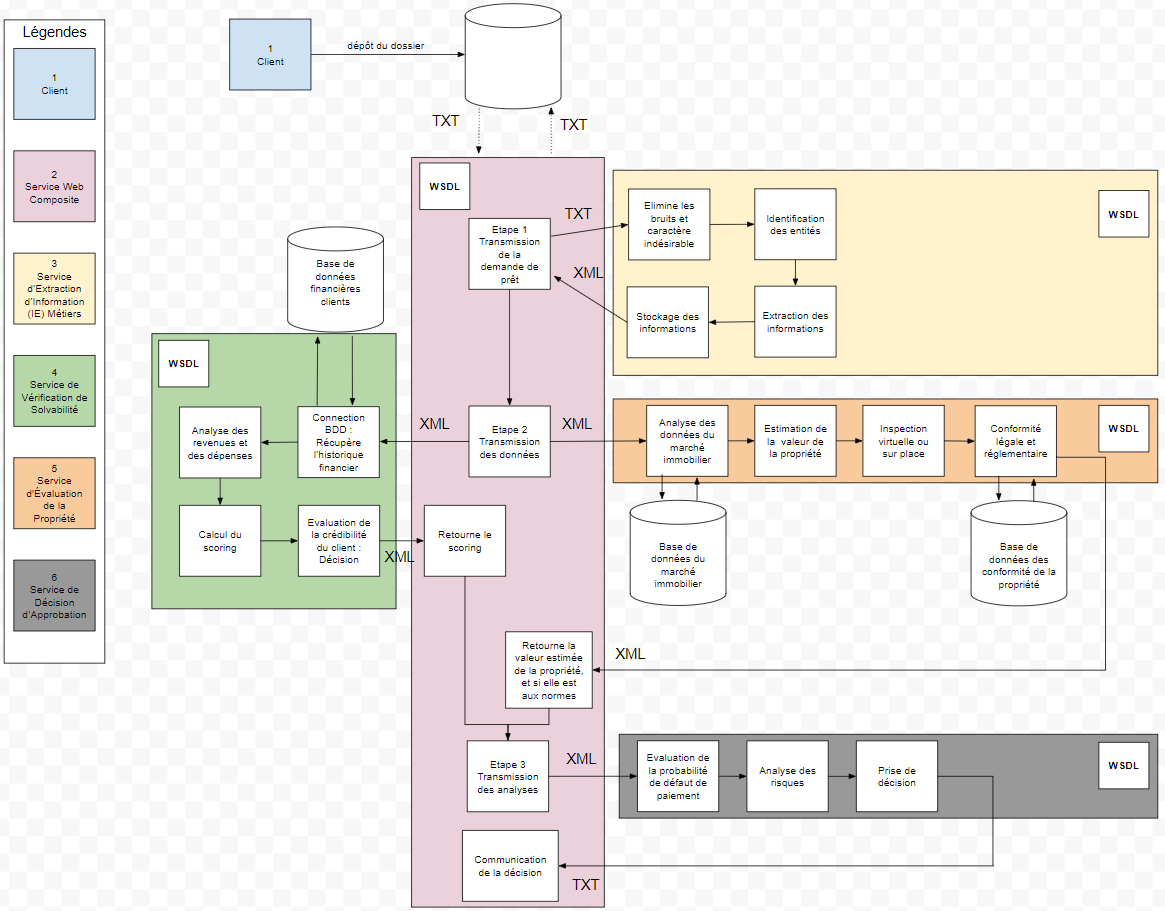
\includegraphics[width=\textwidth]{Images/6.1/modelisation_XML.png}
 
	\subsection{Fonctionnement interne des services}
	Le service \textbf{Composite} permet les échanges entre les services et les échanges avec le client et organise le SOAP. \\
	\\
	Le service d’\textbf{Extraction} prend en paramètre le fichier \texttt{txt} de la demande du client.\\
	Ce service va récupérer les informations indiquées dans le fichier \texttt{txt}, supprime les caractères indésirables et extrait les données après le caractère " : ".\\
	Une fois extraites, les données sont écrites dans des balises correspondantes dans un fichier \texttt{XML}. \\
	Le fichier \texttt{XML} sera nommé selon le numéro de dossier attribué au client. \\
	\\
	Le service de \textbf{Vérification de Solvabilité} prend en paramètre le fichier \texttt{XML} concernant la demande du client. \\
	Ce service va récupérer les informations concernant le montant et la durée du prêt ainsi que les revenus et les dépenses mensuelles à l'aide du numéro de dossier du client. \\
	Il va également récupérer le fichier \texttt{json} banque : \\
	(\texttt{idBanque, age, enfants, emploi, nbCreditsEnCours, antecedents, tauxEndettement}) où : 
	\begin{itemize}
		\item \texttt{idBanque} est l’identifiant de la banque du client
		\item \texttt{age} est l’âge du client
		\item \texttt{enfants} est le nombre d’enfants à sa charge
		\item \texttt{emploi} est un booléen avec 0 si l’emploi n’est pas stable, 1 sinon
		\item \texttt{nbCreditsEnCours} est le nombre de crédits totaux toujours en cours
		\item \texttt{antecedents} est le nombre d’antécédents à son actif (dettes non payées, retards…) 
		\item \texttt{tauxEndettement} est le taux d’endettement actuel
	\end{itemize}
	Le service va ensuite extraire les données en prenant le tuple correspondant à l’\texttt{idBanque} du fichier \texttt{XML} et faire un scoring en fonction des informations. \\
	La décision sera immédiatement "Non Admissible" si le client a moins de 18 ans ou si sa capacité d’emprunt ajouté à ses dépenses est supérieure à son revenu ou encore si son taux d’endettement est supérieur à 33\%.\\
	Une fois l’algorithme de scoring effectué, le service va déterminer en fonction du score, une décision : 
	\begin{itemize}
		\item entre 0 et 10 : peu probable
		\item entre 10 et 20 : à défendre
		\item entre 20 et 30 : sous conditions
		\item  entre 30 et 40 : très favorable
	\end{itemize}
	Finalement, le service ajoute au fichier \texttt{XML} reçu, les balises \texttt{<scoring>Valeur du score</scoring>} et \texttt{<decisionScoring>Decision en fonction du score</decisionScoring>}.\\
 \\
	Le service  d'\textbf{Évaluation de la Propriété} prend en paramètre le fichier \texttt{XML} selon la demande du client. \\
	Le service vérifie si la propriété est conforme aux normes légales et réglementaires en vigueur. \\
	Il va pour cela, récupérer l’adresse de la propriété puis récupérer le fichier \texttt{json} immobilier : \\
	(\texttt{idImmobilier, adresse, age, normeLegal, normeReglementaire, litigesEnCours,\\ normeElectricite, normeGaz}) où : 
	\begin{itemize}
		\item \texttt{idImmobilier} est l’identifiant de la propriété
		\item \texttt{adresse} est l’adresse de la propriété
		\item \texttt{age} est l’âge de la propriété
		\item \texttt{normeLegal} est un booléen avec 0 si la propriété est aux normes, 1 sinon
		\item \texttt{normeReglementaire} est un booléen avec 0 si la propriété est aux normes, 1 sinon 
		\item \texttt{litigesEnCours} est le nombre de litiges en cours
		\item \texttt{normeElectricite} est la norme électrique ("NFC 15-100", "NF C 15-100" ou "C 15-100")
		\item \texttt{normeGaz} est la norme pour le gaz (‘NF P 45-500’ ou vide s’il n’y a pas de gaz dans la propriété)
	\end{itemize} 
	
	Le service va ensuite extraire les données en prenant le tuple correspondant à l’adresse du fichier \texttt{XML} et vérifier que tout est conforme : soit 0, soit dans les normes définies. \\
	Si l’un des attributs n’est pas aux normes, la décision est "Non Admissible à un prêt" et liste les raisons pour lesquelles la propriété pose problème. \\
	Il ajoute au fichier \texttt{XML} reçu la balise : \\
	\\
	\texttt{<decisionConformite>\\
	Decision en fonction du respect ou non des normes\\
	</decisionConformite>} \\
	\\
	Si la décision est "Non admissible", il ajoute aussi une balise : \\
	\\
	\texttt{<raisons>Liste des raisons du refus</raisons>}.\\
	\\
	Le service peut demander à faire une visite virtuelle ou sur place, on considère que si le service demande une visite, il effectue d'abord une visite virtuelle, si celle-ci n’est pas concluante, il demande alors un expert pour une visite sur place. \\
	Le service va choisir un entier aléatoire entre 0 et 1 pour savoir s’il fait une visite. \\
	Si  c’est 0, il ne fait aucune demande de visite, sinon il enclenche une visite virtuelle. \\
	Par la suite, on suppose qu’il va faire une visite sur place uniquement si l'âge de la propriété est inférieur à 10 ans (il n’est plus nécessaire d’avoir un certificat de conformité si la propriété a plus de 10 ans). \\
	En fonction des résultats précédents vis-à-vis de la conformité, la visite sur place est déterminée concluante ou non.\\
	Le service va aussi estimer la valeur marchande de la propriété pour laquelle le prêt est demandé. \\
	Il va récupérer le code postal de l’adresse puis récupérer le type de bâtiment (maison/appartement) et, s'il est donné, le nombre d’étages, avec la \texttt{descriptionPropriete} du fichier \texttt{XML}. \\
	Ensuite il récupère le fichier \texttt{json} \texttt{marcheImmobilier} : \\ 
	(\texttt{adresse, codePostal, batiment, nbEtage, valeur}) où : 
	\begin{itemize}
		\item \texttt{adresse} est l’adresse de la propriété
		\item \texttt{codePostal} est le code postal
		\item \texttt{batiment} est le type de bâtiment
		\item \texttt{nbEtage} est le nombre d’étages
		\item \texttt{valeur} est la valeur marchande de la propriété
	\end{itemize}
	Le service va récupérer tous les tuples qui correspondent au même code postal que celui du fichier \texttt{XML} ainsi que le même type de bâtiment, le nombre d’étages s’il est donné et faire une moyenne de leur valeur. \\
	Finalement, il ajoute au fichier \texttt{XML} reçu, la balise :\\
	\texttt{<estimation\_valeur> \\
	Valeur moyenne des bâtiments du même type et dans le même secteur\\
	</estimation\_valeur>}\\
	\\
	Le service  de \textbf{Décision d’Approbation} prend en paramètre le fichier \texttt{XML} concernant la demande du client. \\
	Ce service va récupérer les informations concernant le montant du prêt, le score, la décision du score, la décision de conformité (les raisons pour lesquelles c’est un refus si c'en est un) ainsi que l’estimation de la valeur. 
	\begin{itemize}
		\item Si la valeur du score est -1, le score n’a pas été calculé à cause de sa situation financière, le prêt est refusé.
		\item Si la décision de conformité est "Non admissible à un prêt immobilier", le service émet le refus du prêt avec une liste de raisons.
		\item Si le montant est supérieur à l’estimation de la valeur en plus d'une valeur choisie arbitrairement, le service émet un refus avec les raisons que le montant demandé est trop important pour la propriété.
	\end{itemize}
	
	Par la suite en fonction de la décision du score, \\
	s’il s’agit de "Très favorable", "Sous conditions" ou "À défendre" et que la décision de conformité est aussi "Admissible à un prêt immobilier" alors le service accepte la demande, sinon il la refuse.\\
	En fonction des résultats précédents, le service a pris une décision d'approbation ou de refus du prêt puis communique celle-ci au service \textbf{Composite} (en indiquant les raisons du refus du prêt) sous la forme d’un fichier \texttt{txt} qui sera stocké dans le répertoire \texttt{reponseTxt}.
	
 \section{Implémentation avec SOAP}
	\subsection{Structure du projet}
 
    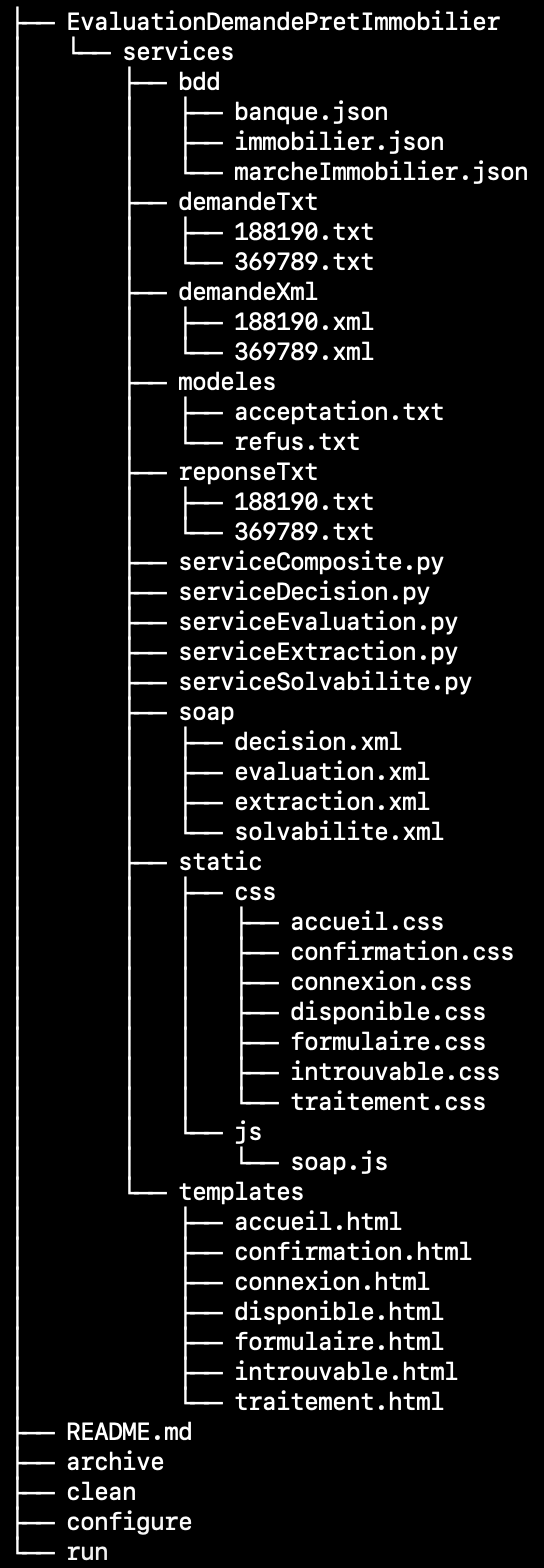
\includegraphics[width=225pt]{Images/7.1/tree.png}\\
    \begin{itemize}
    \item Dans le dossier \texttt{ProjetSOAP}, nous avons:
    \begin{itemize}
        \item un dossier \texttt{EvaluationDemandePretImmobilier}, contenant le coeur du projet;
        \item un \texttt{README.md}, donnant les commandes et les scénarios à exécuter;
        \item et des scripts (\texttt{archive, clean, configure, run}).
    \end{itemize}  
    
    \item Dans le dossier \texttt{EvaluationDemandePretImmobilier},  nous avons un dossier \texttt{services} contenant le coeur du projet. 
    
    \item Le projet se situant dans le dossier \texttt{services}, il est composé de:
    \begin{itemize}
      \item un dossier \texttt{bdd} contenant l'ensemble des bases de données (\texttt{banque, immobilier, marcheImmobilier}) en format \texttt{json};
      \item un dossier \texttt{demandeTxt} contenant les formulaires à traiter, soumis par les clients sur l'interface web, en format \texttt{txt};
      \item un dossier \texttt{demandeXml} contenant les demandes en cours d'évaluation, crée dans l'extraction des données et utilisés par les autres services, en format \texttt{XML};
      \item un dossier \texttt{modeles} contenant les modèles de textes pour générer le résultat, 2 versions : acceptation et refus;
      \item un dossier \texttt{reponseTxt} contenant les résultats obtenus suite à l'évaluation du prêt;
      \item un dossier \texttt{soap} qui contient les messages SOAP envoyés en interaction entre 2 services sous format \texttt{XML} (ex : \texttt{extraction.xml} qui est le message de communication entre le service composite et le service extraction);
      \item un dossier \texttt{static} qui contient l'ensemble des fichiers \texttt{CSS} et \texttt{JS} nécessaire pour l'interface web;
      \item un dossier \texttt{templates} qui contient l'ensemble des fichiers \texttt{HTML} contenant les pages web de l'interface;
      \item ainsi que les fichiers \texttt{.py} pour chaque service tels que : \texttt{serviceComposite.py, serviceDecision.py, serviceEvaluation.py, serviceExtraction.py, serviceSolvabilite.py} .
    \end{itemize}
    
    \end{itemize}
    
	\subsection{Spécifications des services}
    \subsubsection{Service Composite}
      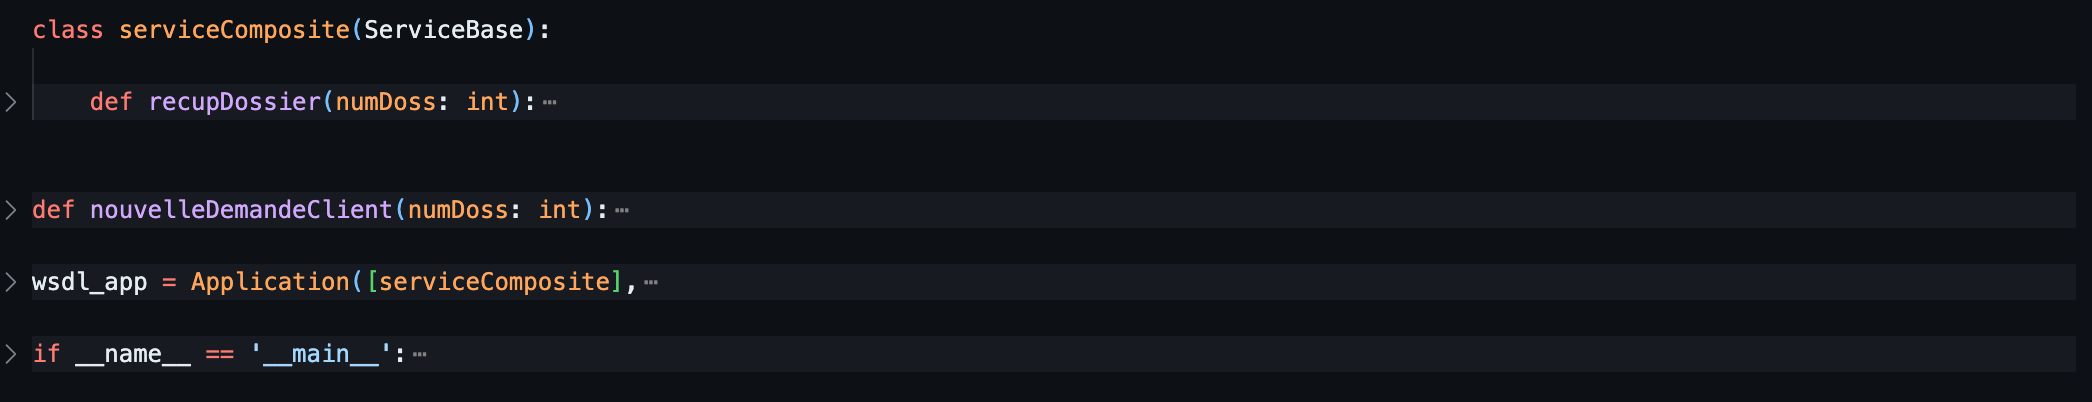
\includegraphics[width=\textwidth]{Images/7.2/serviceComposite.png}\\
      \\ 
      Le \texttt{service Composite} est l'orchestrateur de ce projet. Il permet de lancer l'évaluation de la demande de prêt et de faire appel aux autres services (Extraction, VerificationSolvabilité, EvaluationPropriété, Décision). Il contient les fonctions suivantes:
      \begin{itemize}
          \item \texttt{recupDossier} : permet de récupérer le formulaire en fichier \texttt{txt} dans le dossier \texttt{demandeTxt} pour lancer l'évaluation de prêt;
          \item \texttt{nouvelleDemandeClient} : permet de communiquer avec les autres services après lancement de l'évaluation de demande de prêt.
      \end{itemize}
    \subsubsection{Service Extraction}
      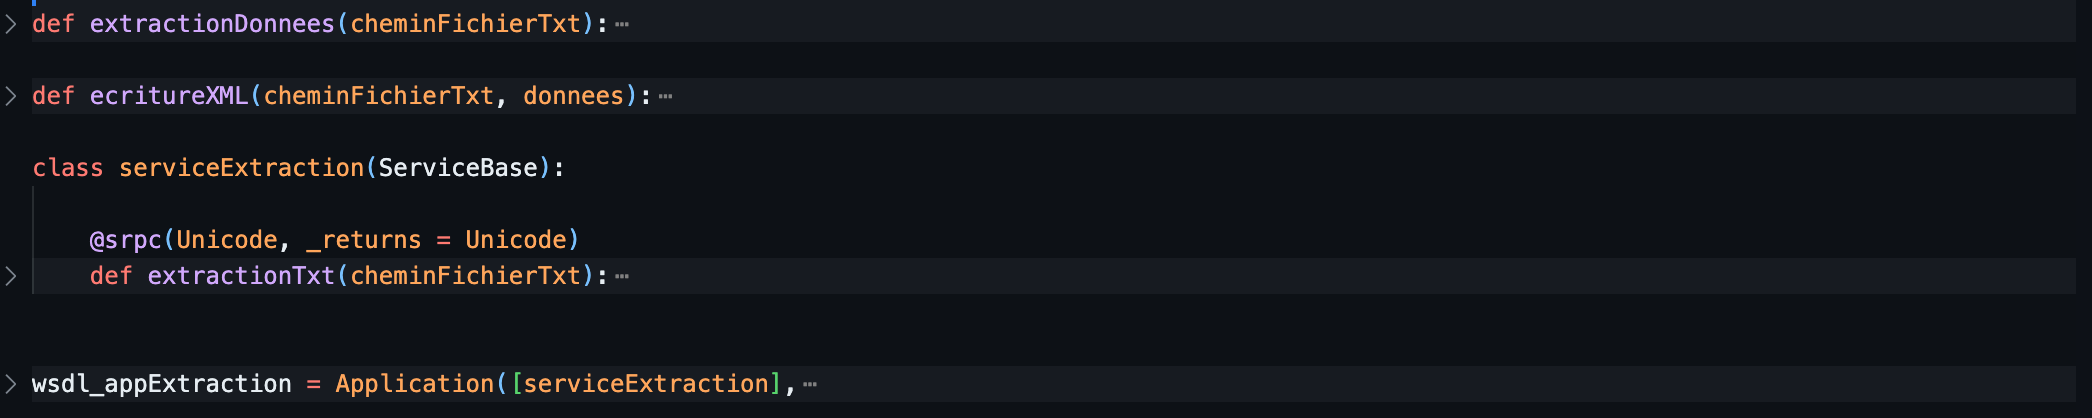
\includegraphics[width=\textwidth]{Images/7.2/serviceExtraction.png}\\
      \\
      Le \texttt{service Extraction} permet d'extraire un fichier \texttt{.txt} (formulaire) en entités, de récupérer les entités nécessaires pour l'évaluation du prêt et d'enregistrer dans un fichier \texttt{.xml}. Il contient les fonctions suivantes:
      \begin{itemize}
          \item \texttt{extractionDonnees} : permet d'extraire en entités un fichier \texttt{.txt};
          \item \texttt{ecritureXML} : permet de créer un nouveau fichier \texttt{.xml} et de remplir entre chaque balise les entités extraites dans la fonction précédente;
          \item \texttt{extractionTxt} : fonction de la classe \texttt{ServiceExtraction} qui permet d'appliquer les 2 fonctions précédentes.
      \end{itemize}
    \subsubsection{Service Solvabilité}
      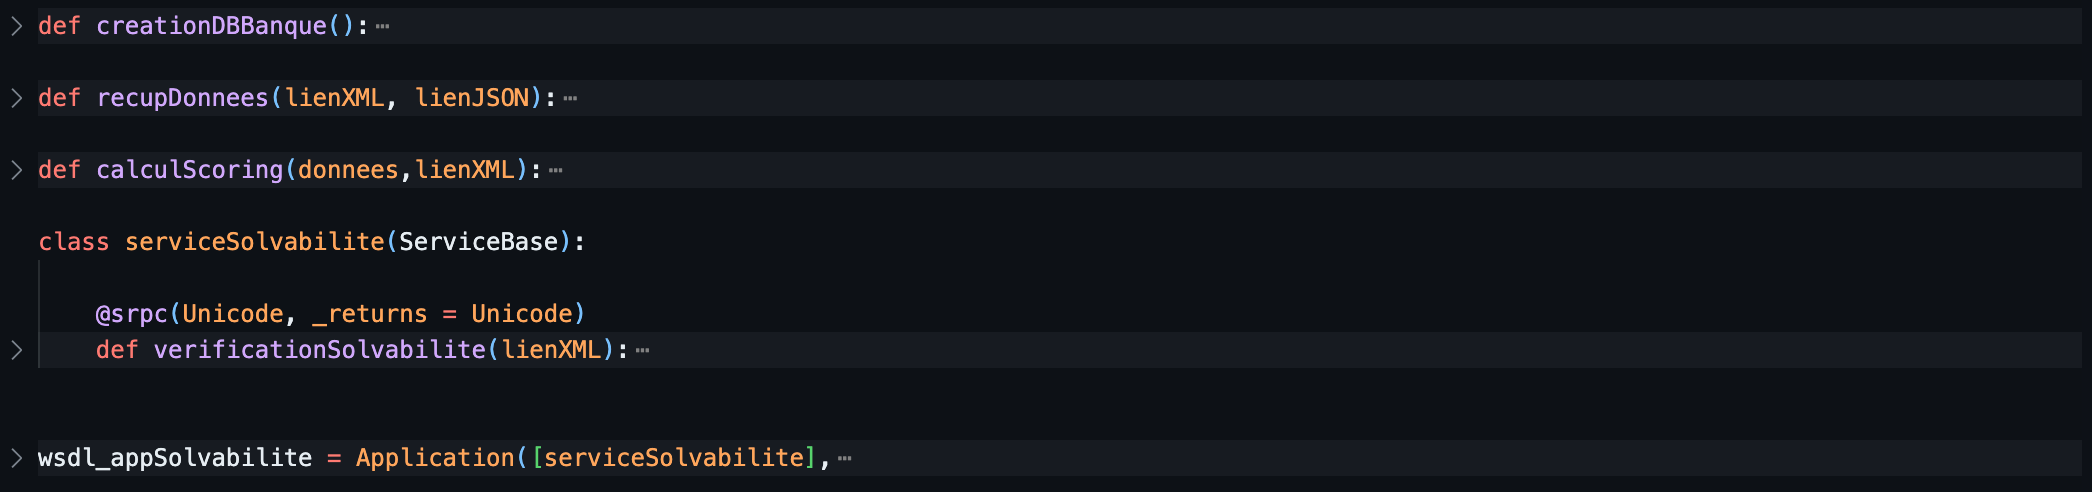
\includegraphics[width=\textwidth]{Images/7.2/serviceSolvabilite.png}\\
      \\
      Le \texttt{service Solvabilité} permet de vérifier la solvabilité en fonction de la situation financière du demandeur de prêt. Pour cela, il va recueillir les données nécessaires du client et calculer le scoring avec ces données. Il contient les fonctions suivantes:
      \begin{itemize}
          \item \texttt{creationDBBanque} : permet de créer un fichier \texttt{JSON} qui contient la base de données \texttt{Banque};
          \item \texttt{recupDonnees} : permet de récupérer les données concernant le client et sa situation financière provenant de la base de données \texttt{Banque};
          \item \texttt{calculScoring} : permet de calculer le scoring du client en fonction des données récupérées dans la fonction précédente et d'écrire le score ainsi que la décision du score dans le fichier \texttt{.xml} du dossier \texttt{demandeXML/};
          \item \texttt{verificationSolvabilite} : fonction de la classe \texttt{serviceSolvabilite} qui permet d'appliquer les 3 fonctions précédentes.
      \end{itemize}
    \subsubsection{Service Évaluation}
      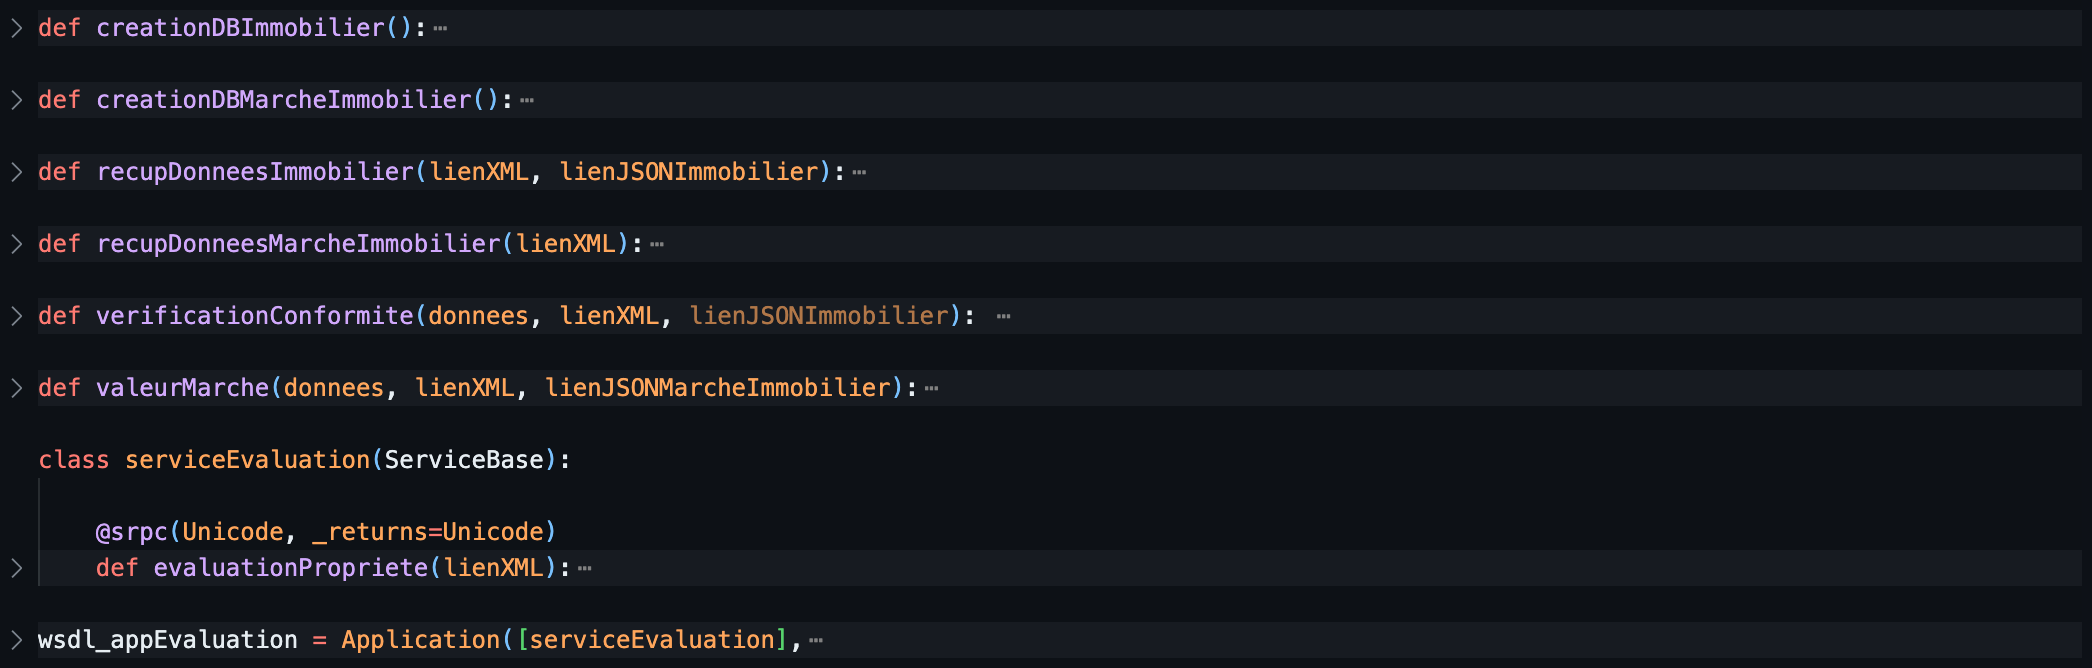
\includegraphics[width=\textwidth]{Images/7.2/serviceEvaluation.png}\\
      \\
      Le \texttt{serviceEvaluation} permet d'évaluer la propriété pour laquelle le client demande son prêt. Pour cela, il va dans un premier temps vérifier la conformité de la propriété et ensuite vérifier la valeur de cette propriété dans le marché. Il contient les fonctions suivantes:
      \begin{itemize}
          \item \texttt{creationDBImmobilier} : permet de créer un fichier \texttt{JSON} qui contient la base de données \texttt{Immobilier};
          \item \texttt{creationDBMarcheImmobilier} : permet de créer un fichier \texttt{JSON} qui contient la base de données \texttt{MarcheImmobilier};
          \item \texttt{recupDonneesImmobilier} : permet de récupérer les données concernant les informations de la propriété provenant de la base de données \texttt{Immobilier}; 
          \item \texttt{recupDonneesMarcheImmobilier} : permet de récupérer les données concernant la situation de la propriété provenant du fichier \texttt{.xml} dans le dossier \texttt{demandeXML/};
          \item \texttt{verificationConformite} : permet de vérifier si la situation de la propriété est conforme et légale grâce aux données récupérées dans la fonction précédente et d'écrire la décision de conformité dans le fichier \texttt{.xml} du dossier \texttt{demandeXML/};
          \item \texttt{valeurMarche} : permet de calculer la moyenne des valeurs des propriétés similaires situées dans la même ville en récupérant les données nécessaires dans la base de données \texttt{marcheImmobilier} et d'écrire l'estimation valeur dans le fichier \texttt{.xml} du dossier \texttt{demandeXML/};
          \item \texttt{evaluationPropriete} : fonction de la classe \texttt{serviceEvaluation} qui permet d'appliquer les 6 fonctions précédentes.
      \end{itemize}
    \subsubsection{Service Décision}
      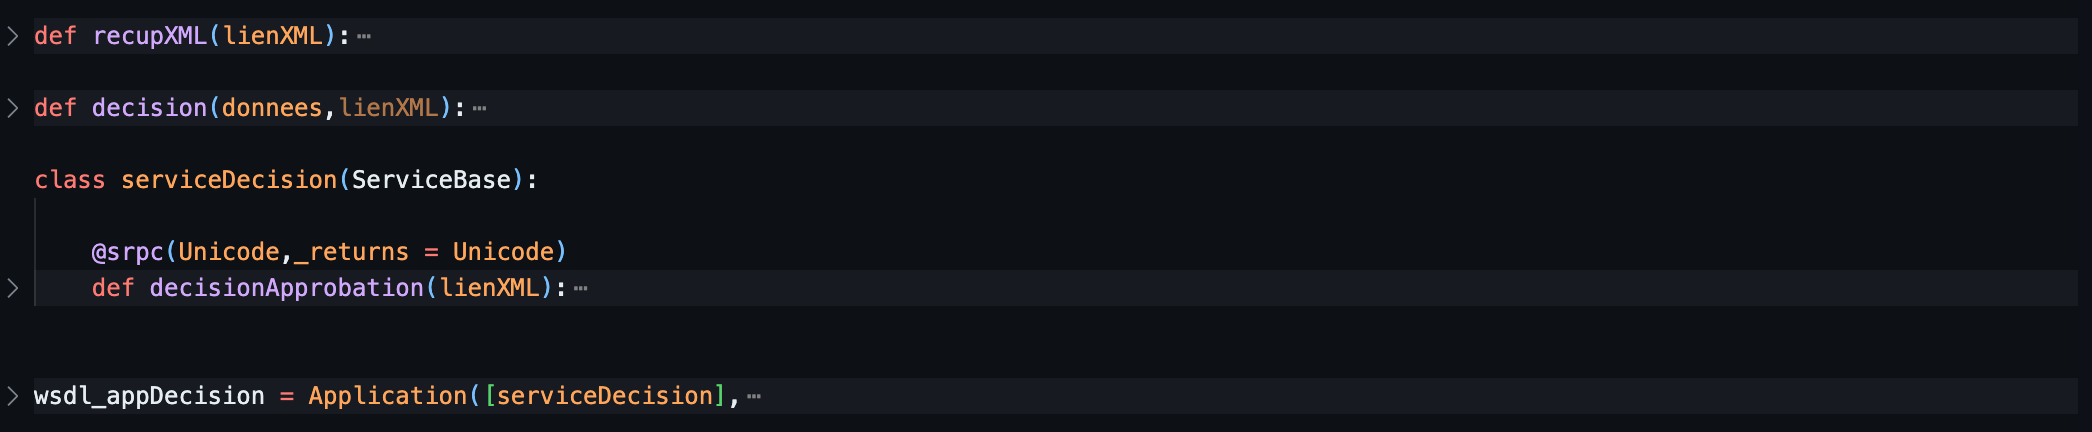
\includegraphics[width=\textwidth]{Images/7.2/serviceDecision.png}\\
    \\
    Le \texttt{serviceDecision} permet de générer une décision suite à l'évaluation du prêt effectué par le \texttt{serviceSolvabilité} et le \texttt{serviceEvaluation}. Il contient les fonctions suivantes:
    \begin{itemize}
        \item \texttt{recupXML} : permet de récupérer les données nécessaires pour pouvoir générer une décision dans le fichier \texttt{.xml} dans le dossier \texttt{demandeXML/};
        \item \texttt{decision} : permet de générer un résultat suite aux évaluations des services précédentes. Ce résultat peut être une acceptation ou un refus. Pour générer le résultat, on se sert des modèles situés dans le dossier \texttt{modeles} et on remplace les données manquantes par les données récupérées dans la fonction précédente. On crée ainsi un fichier \texttt{.txt} dans le dossier \texttt{reponseTxt/} qui sera récupéré par le \texttt{service Composite} pour pouvoir l'afficher sur l'interface lorsque le client lui demande les résultats.
        \item \texttt{decisionApprobation} : fonction de la classe \texttt{serviceDecision} qui permet d'appliquer les 2 fonctions précédentes.
    \end{itemize}
	\subsection{Spécificités de SOAP}
      \subsubsection{Spyne Application} 
        \begin{center}
          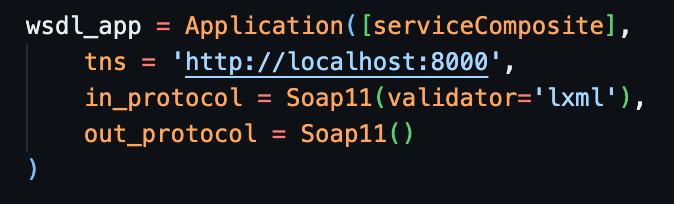
\includegraphics[width=220pt]{Images/7.3/wsdlApp.png}\\
        \end{center}
        \begin{itemize}
            \item Exemple d'une mise en place d'une \texttt{appplication Spyne} (ici pour serviceComposite) qui permet d'appliquer le protocole SOAP entre chaque service.
            \item Chaque service dispose d'une déclaration équivalente à celle-ci. 
        \end{itemize}
      \subsubsection{WSGI Application et WSGI Mounter}
        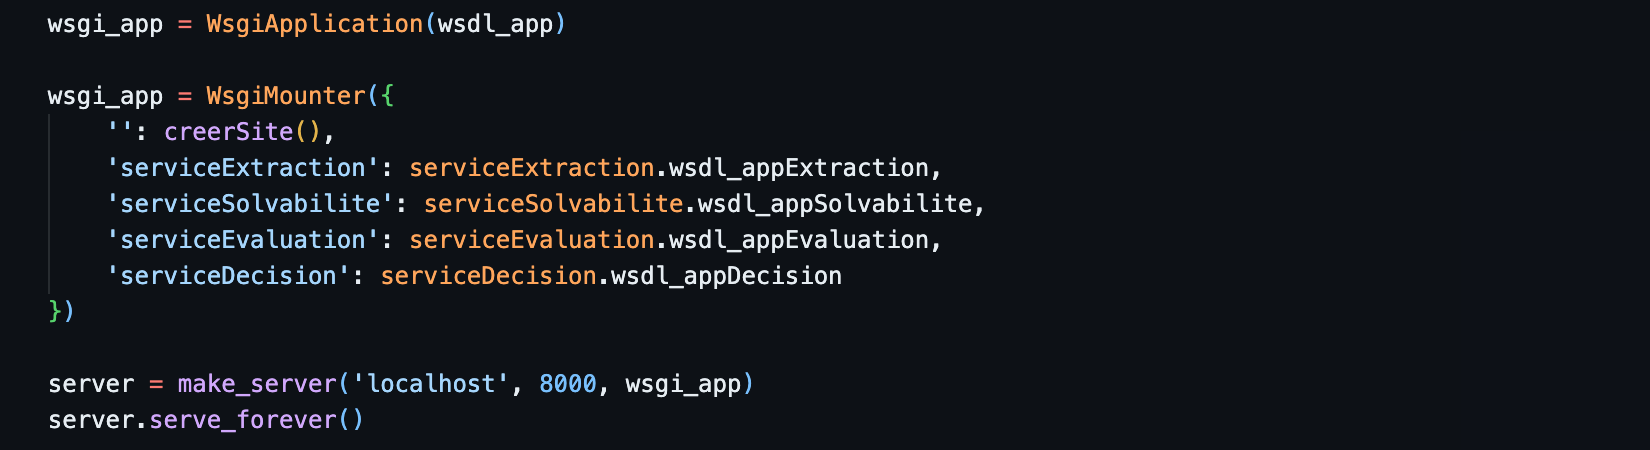
\includegraphics[width=\textwidth]{Images/7.3/wsgiApp_serveur.png}\\
        \begin{itemize}
            \item Déclaration d'une \texttt{WSGI Application} s'appuyant sur une Application Spyne
            \item Montage des services avec leurs endpoints respectifs grâce à \texttt{WSGI Mounter}
            \item Démarrage du serveur sur le port 8000 de l'Application Spyne
        \end{itemize}

      \subsubsection{Interaction entre les services sous le protocole SOAP}
      \begin{itemize}
          \item \textbf{Service Composite $\leftrightarrow$ Service Extraction} \\ \\
          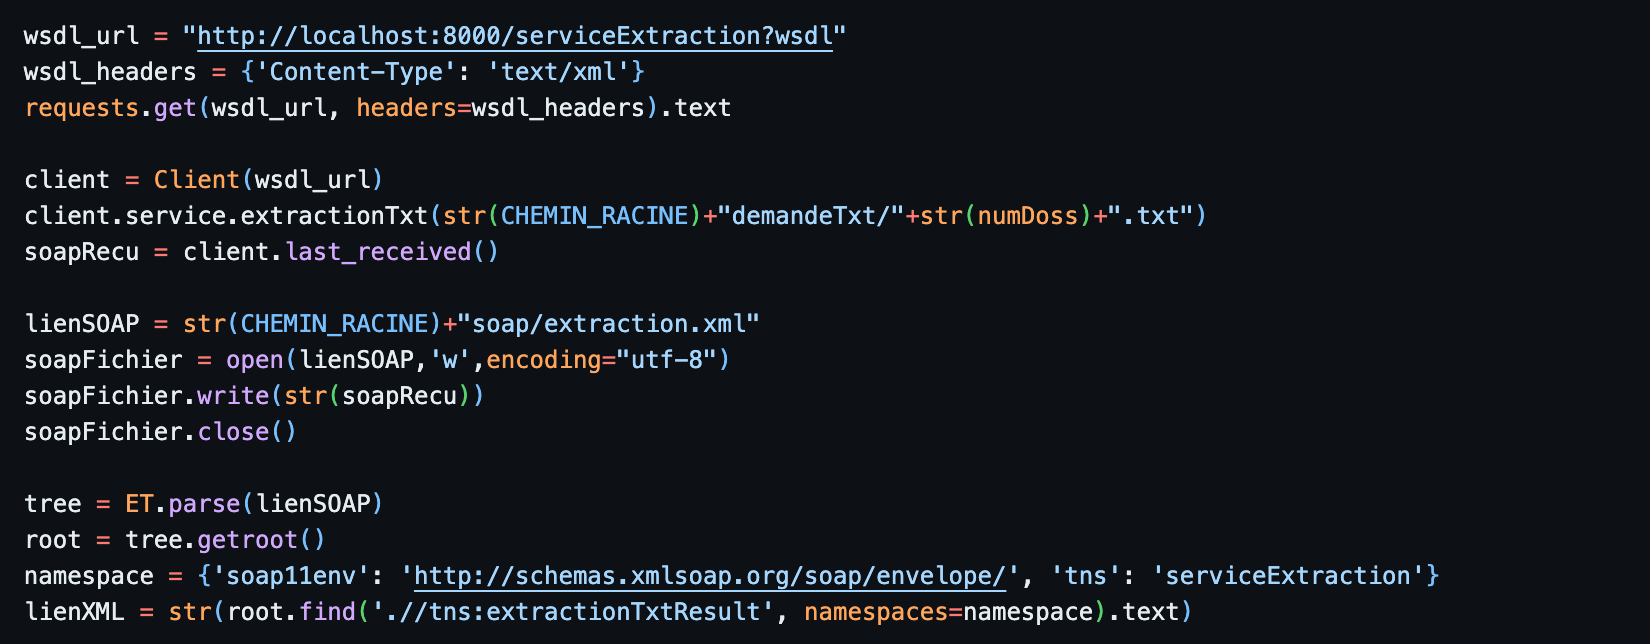
\includegraphics[width=\textwidth]{Images/7.3/wsdlExtraction.png}\\
          \begin{itemize}
              \item Récupération du fichier \texttt{WSDL} du \texttt{serviceExtraction}
              \item Création d'un client à l'aide du module \texttt{suds}
              \item Récupération de la requête SOAP et extraction du lien du fichier \texttt{.XML} dans le dossier \texttt{demandeXML/} dans le \texttt{serviceComposite}
          \end{itemize}
          \textbf{Enveloppe SOAP générée : \texttt{extraction.xml}}\\ \\
          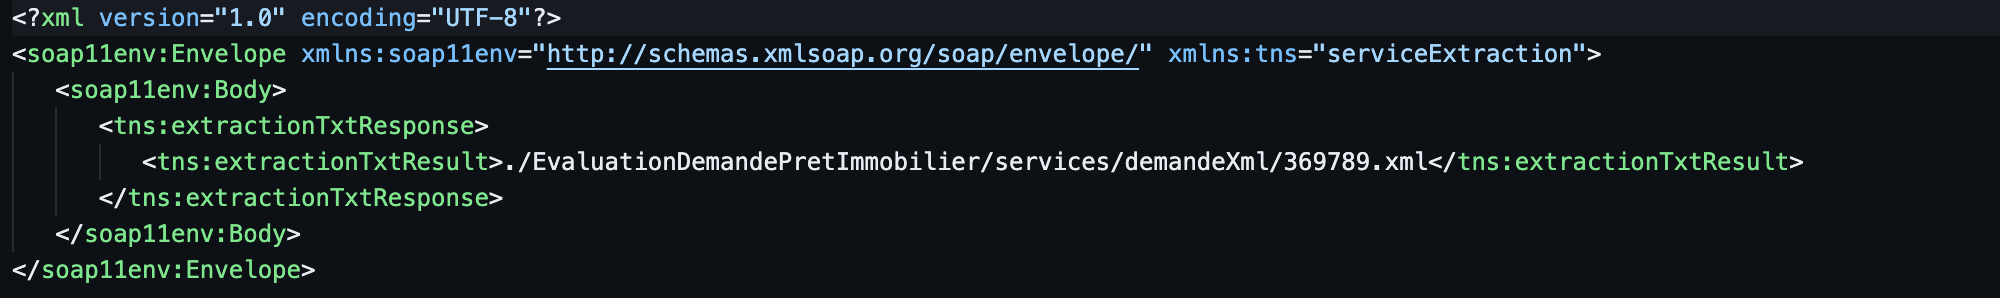
\includegraphics[width=\textwidth]{Images/7.3/SOAPExtraction.png}
          
\newpage
          \item \textbf{Service Composite $\leftrightarrow$ Service Solvabilité} \\ \\
          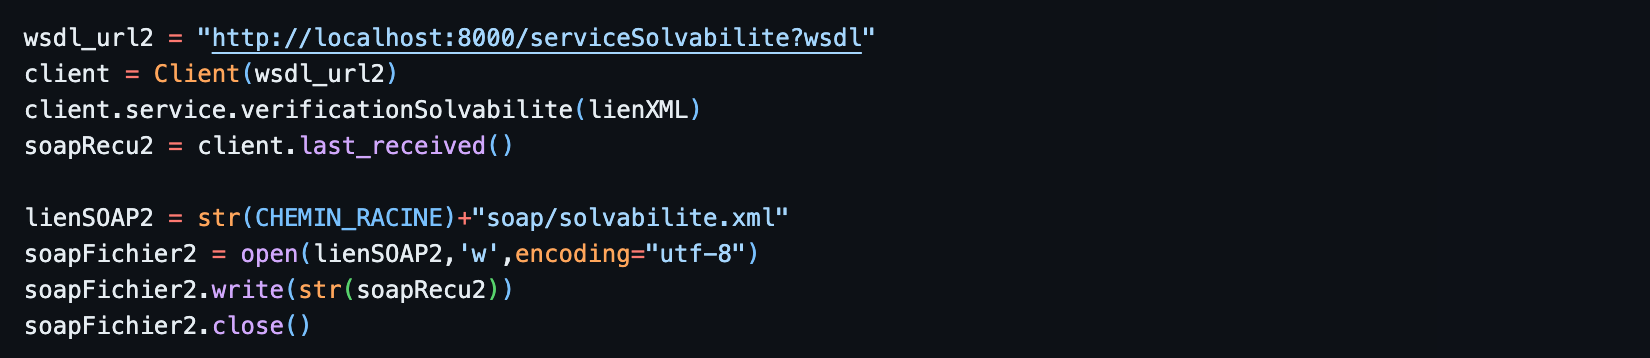
\includegraphics[width=\textwidth]{Images/7.3/wsdlSolvabilite.png}\\
          \begin{itemize}
              \item Récupération du fichier \texttt{WSDL} du \texttt{serviceSolvabilite}
              \item Création d'un client à l'aide du module \texttt{suds}
              \item Récupération de la requête SOAP et écriture du lien du fichier \texttt{.XML} dans le dossier \texttt{demandeXML/} dans le \texttt{serviceComposite}
          \end{itemize}
          \textbf{Enveloppe SOAP générée : \texttt{solvabilite.xml}}\\ \\
          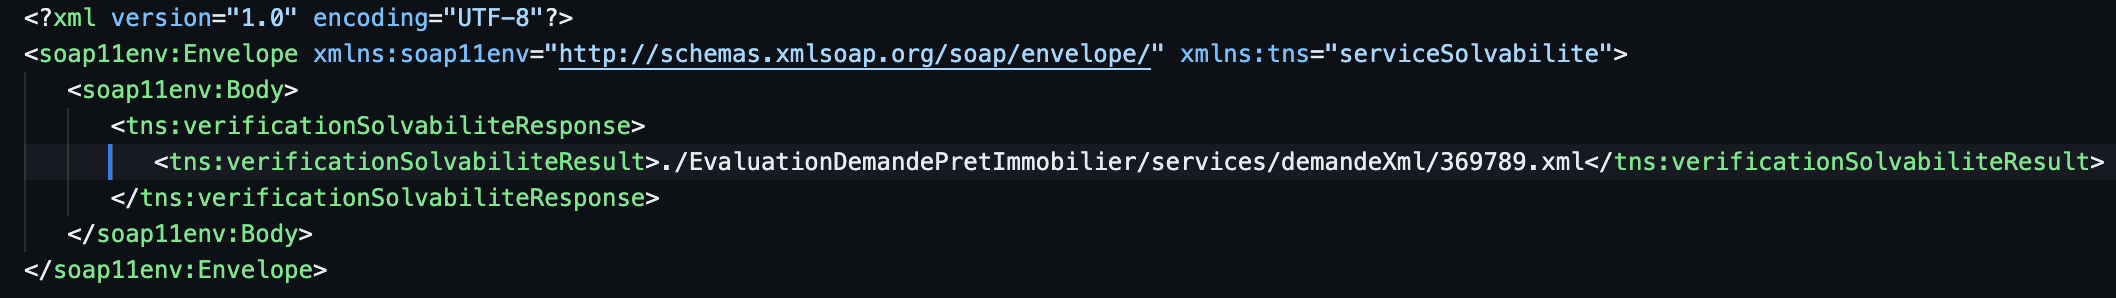
\includegraphics[width=\textwidth]{Images/7.3/SOAPSolvabilite.png}

          
          \item \textbf{Service Composite $\leftrightarrow$ Service Evaluation} \\ \\
          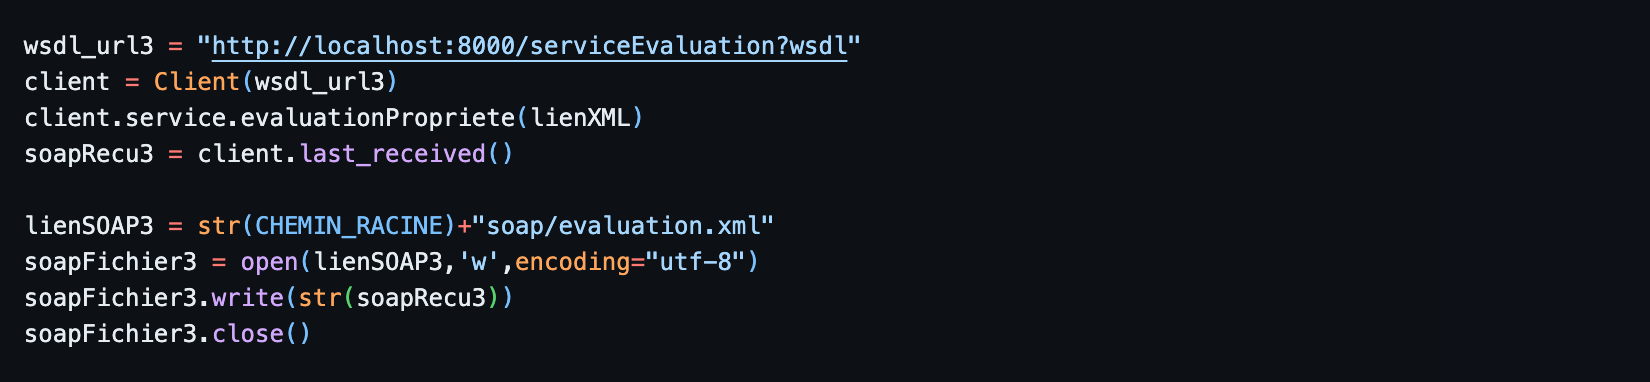
\includegraphics[width=\textwidth]{Images/7.3/wsdlEvaluation.png}\\
          \begin{itemize}
              \item Récupération du fichier \texttt{WSDL} du \texttt{serviceEvaluation}
              \item Création d'un client à l'aide du module \texttt{suds}
              \item Récupération de la requête SOAP et écriture du lien du fichier \texttt{.XML} dans le dossier \texttt{demandeXML/} dans le \texttt{serviceComposite}
          \end{itemize}
          \textbf{Enveloppe SOAP générée : \texttt{evaluation.xml}}\\ \\
          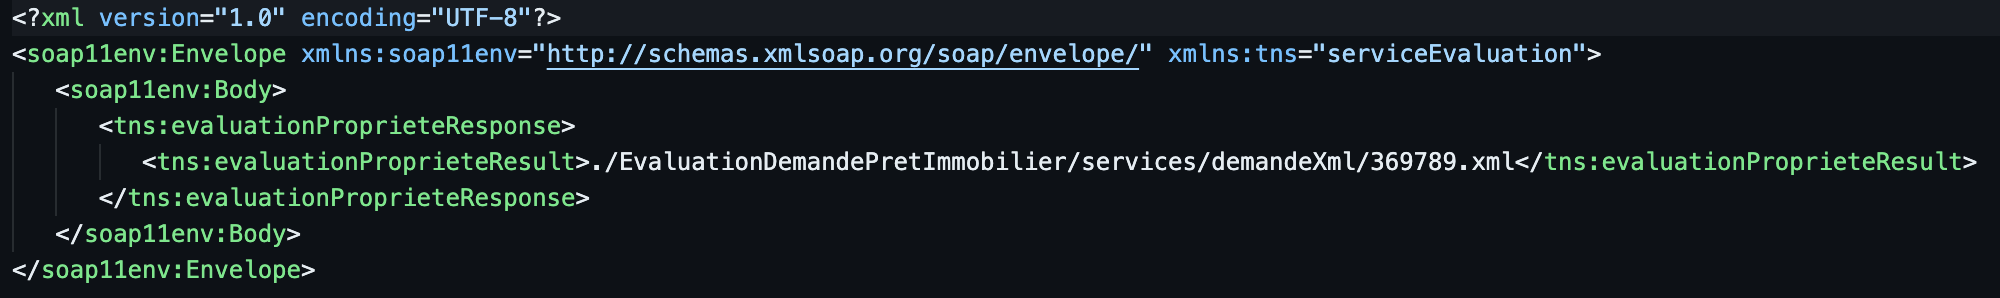
\includegraphics[width=\textwidth]{Images/7.3/SOAPEvaluation.png}
          
\newpage
          \item \textbf{Service Composite $\leftrightarrow$ Service Décision} \\ \\
          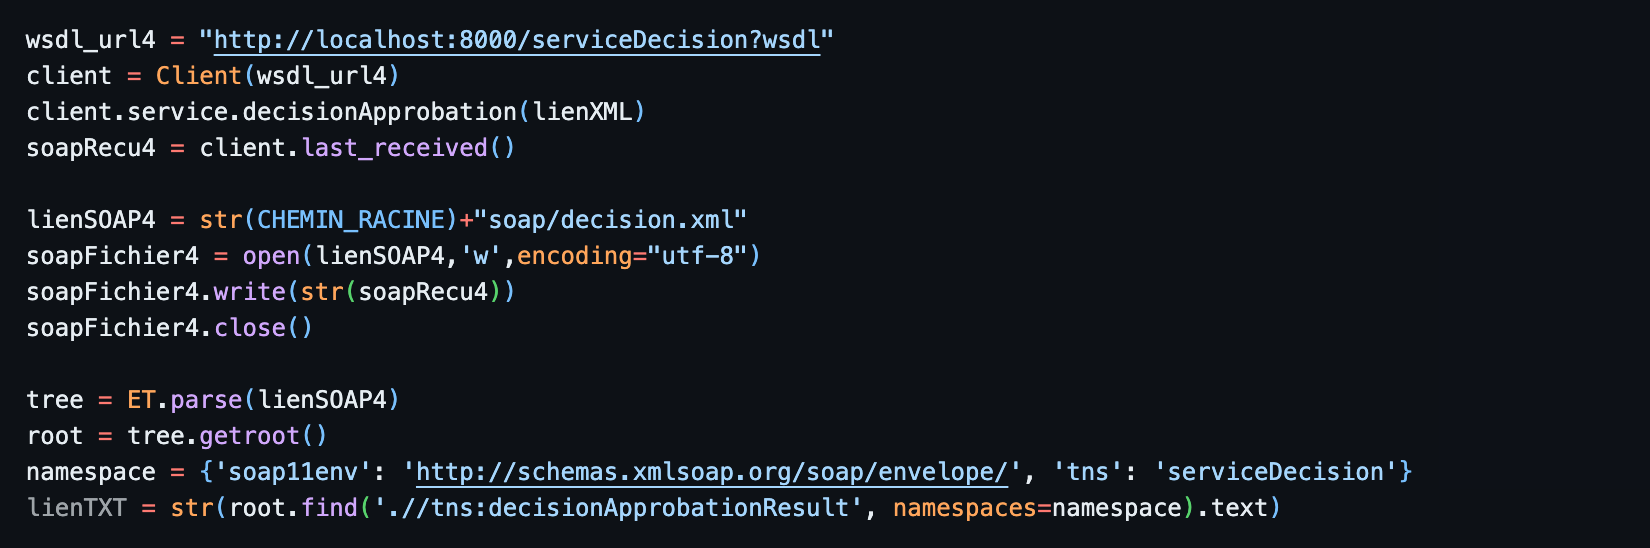
\includegraphics[width=\textwidth]{Images/7.3/wsdlDecision.png}\\
          \begin{itemize}
              \item Récupération du fichier \texttt{WSDL} du \texttt{serviceDecision}
              \item Création d'un client à l'aide du module \texttt{suds}
              \item Récupération de la requête SOAP et écriture du lien du fichier \texttt{.XML} dans le dossier \texttt{demandeXML/} dans le \texttt{serviceComposite}
          \end{itemize}
          \textbf{Enveloppe SOAP générée : \texttt{decision.xml}}\\ \\
          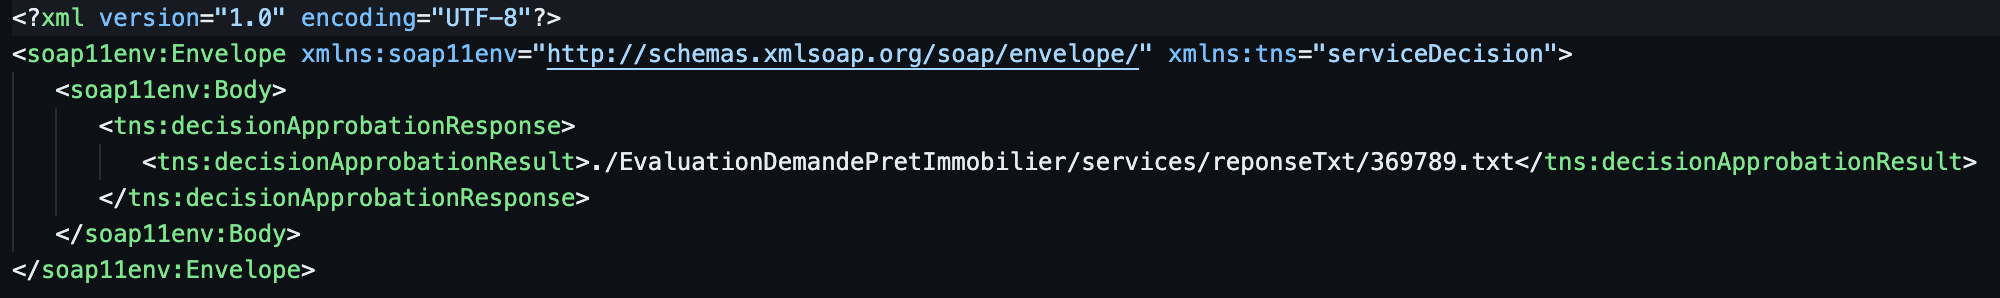
\includegraphics[width=\textwidth]{Images/7.3/SOAPDecision.png}
          
      \end{itemize}

  \newpage

\section{Interface}
    Nous avons effectué une interface afin que le client puisse déposer sa demande de prêt pour l'évaluation et qu'il puisse consulter les résultats.
    
    \subsection{Pages web}
    \subsubsection{Accueil : page d'accueil}
    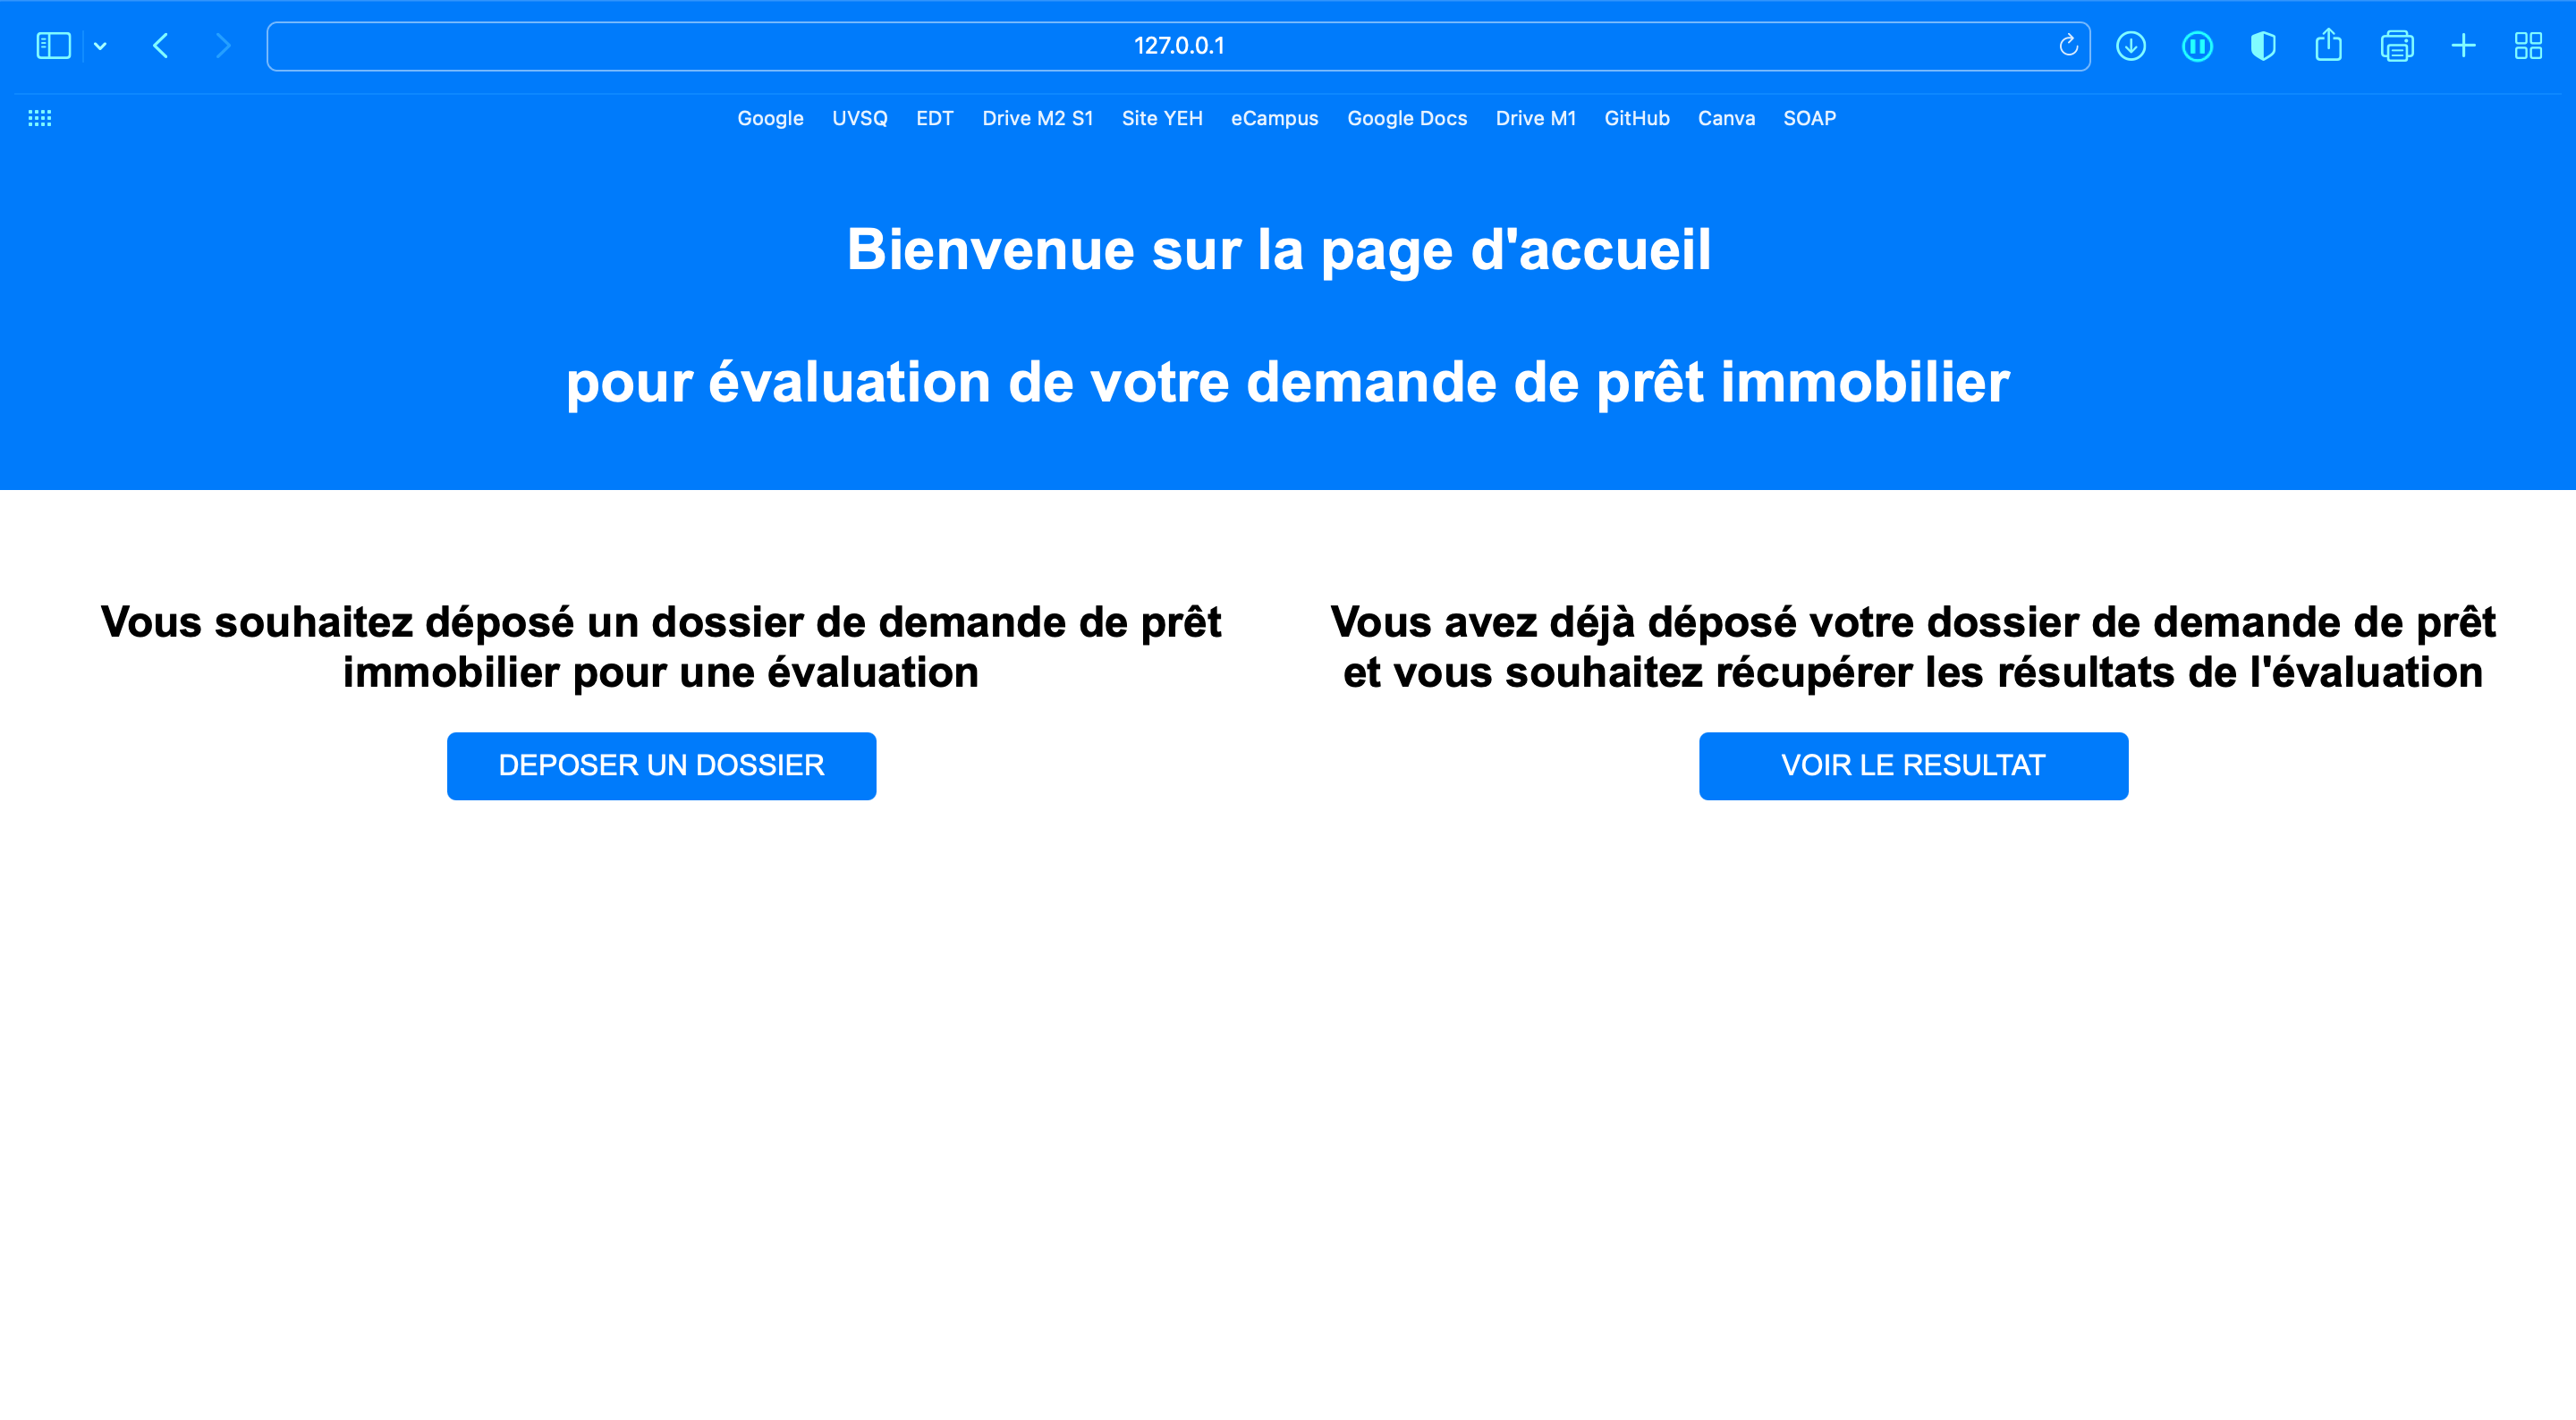
\includegraphics[width=\textwidth]{Images/8.1/accueil.png}
    
    \subsubsection{Formulaire : page contenant le formulaire de demande de prêt à évaluer}
    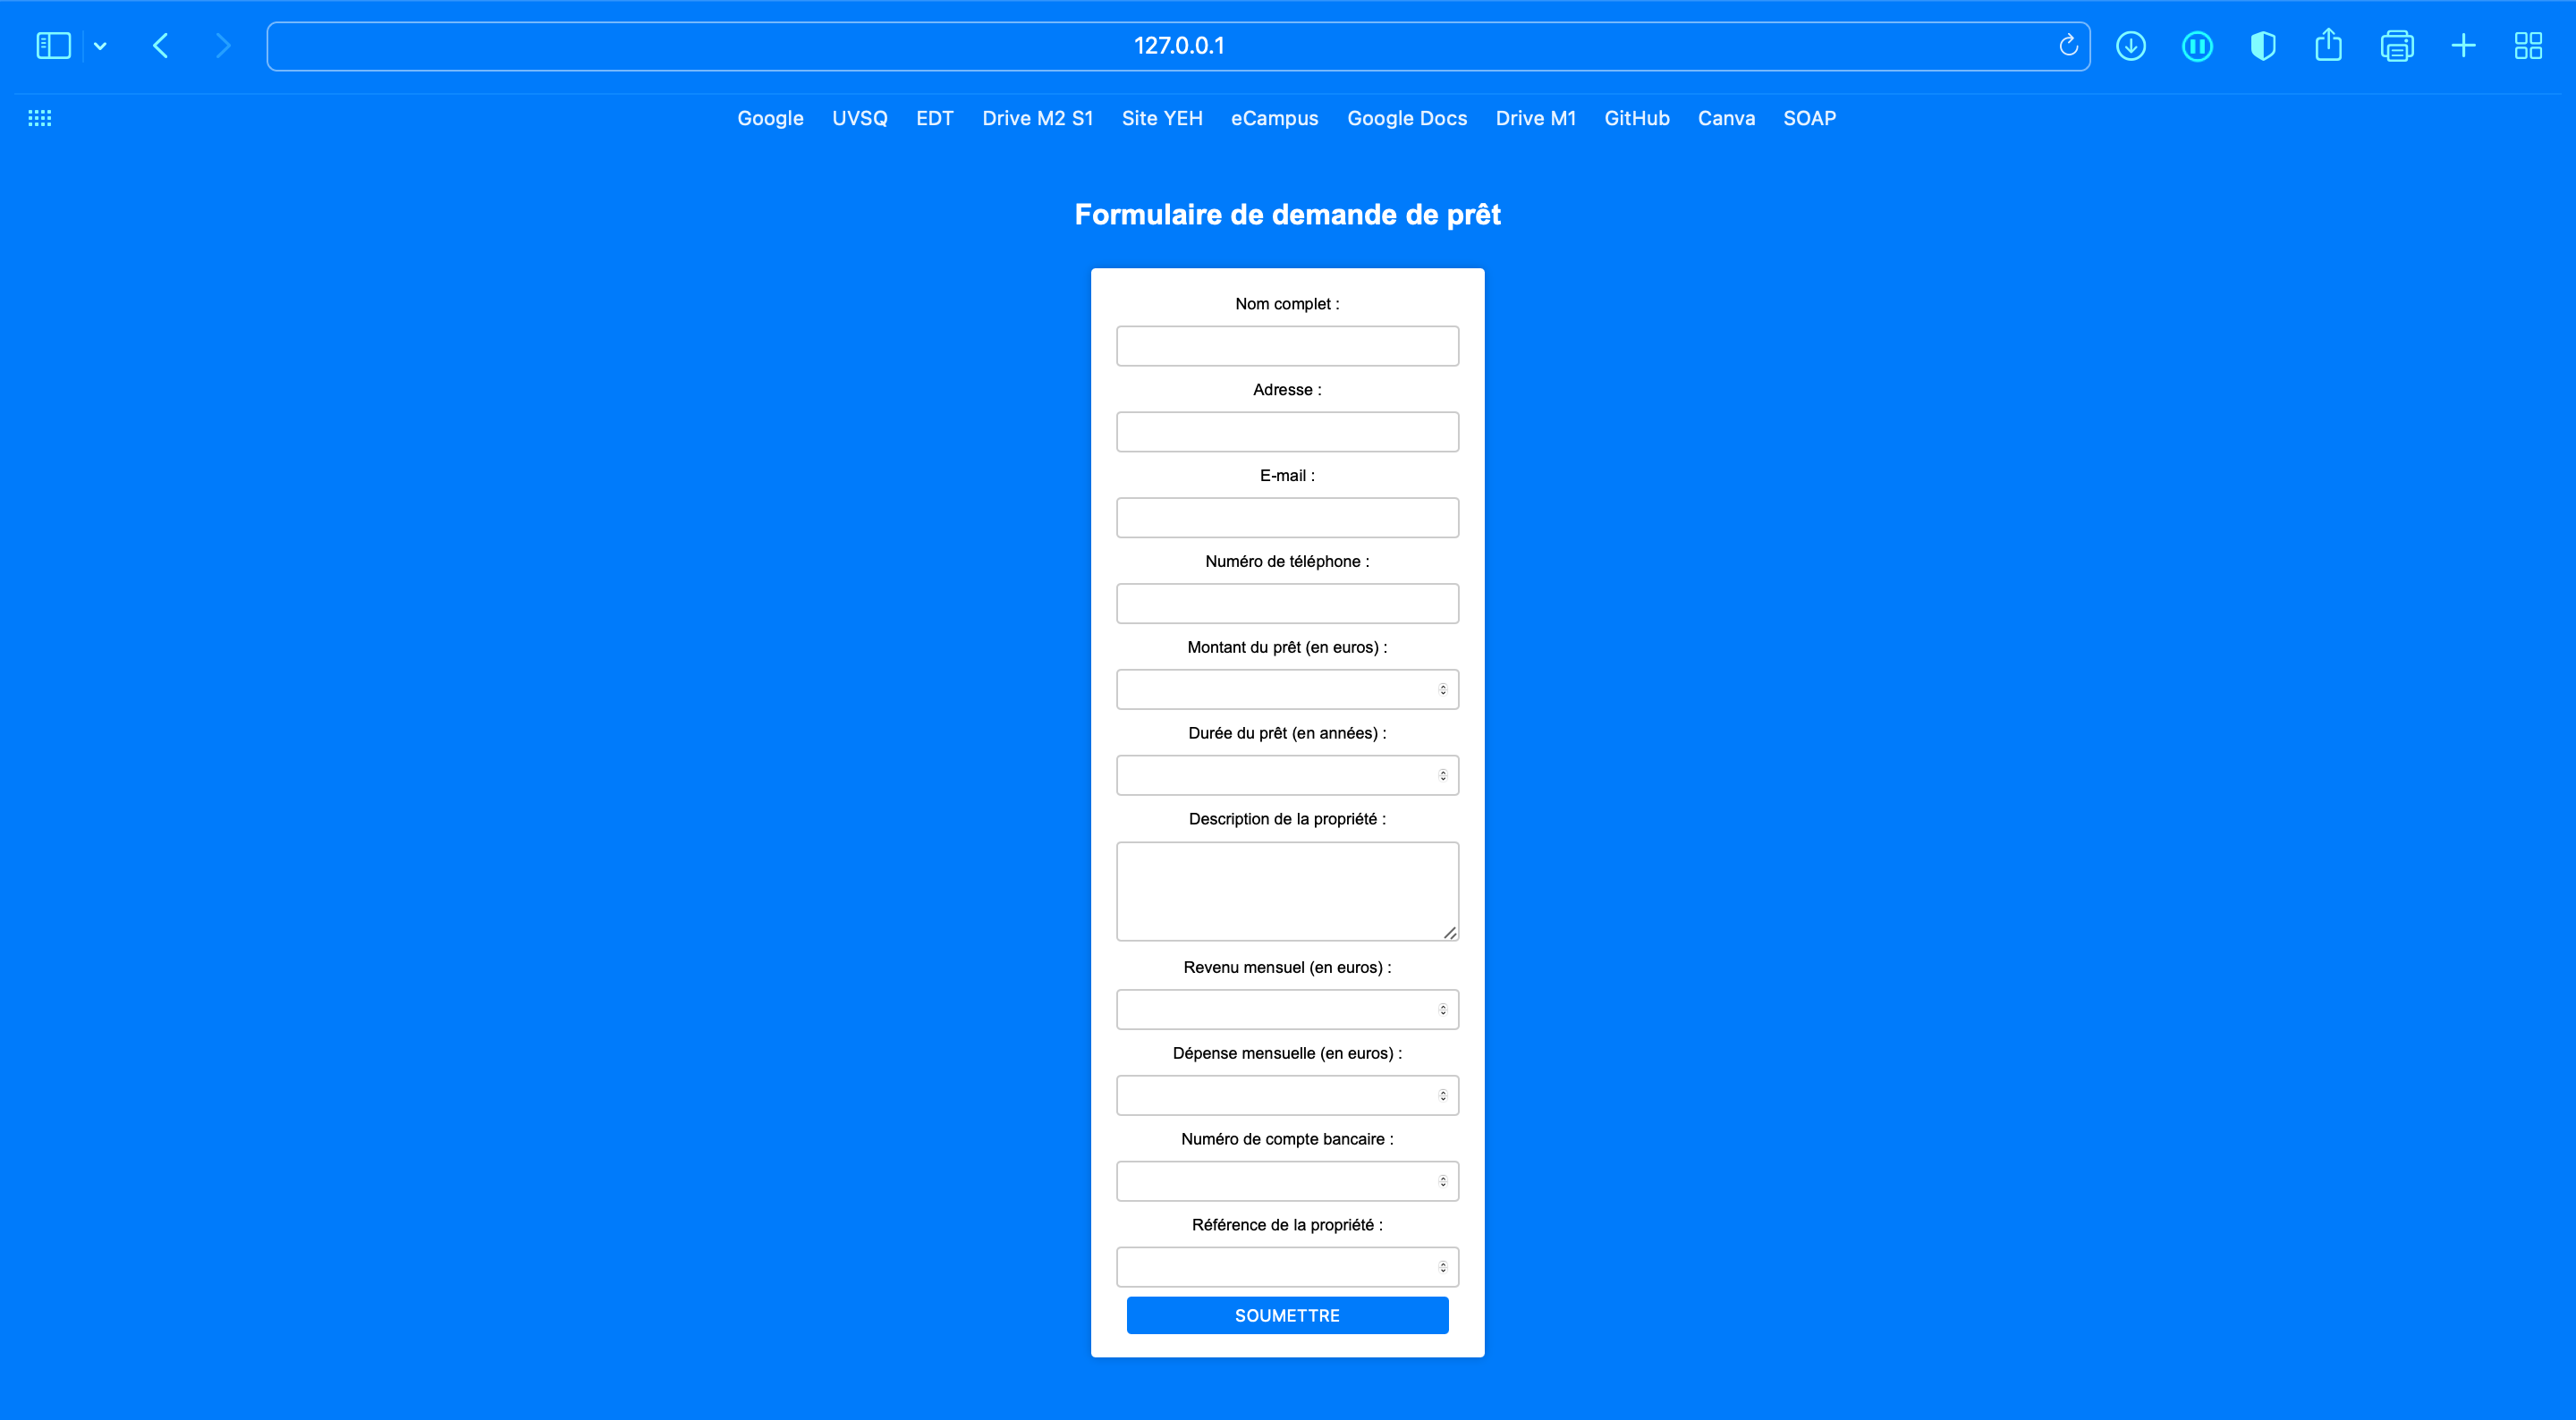
\includegraphics[width=\textwidth]{Images/8.1/formulaire.png}
    
    \subsubsection{Confirmation : page de confirmation de la soumission du formulaire}
    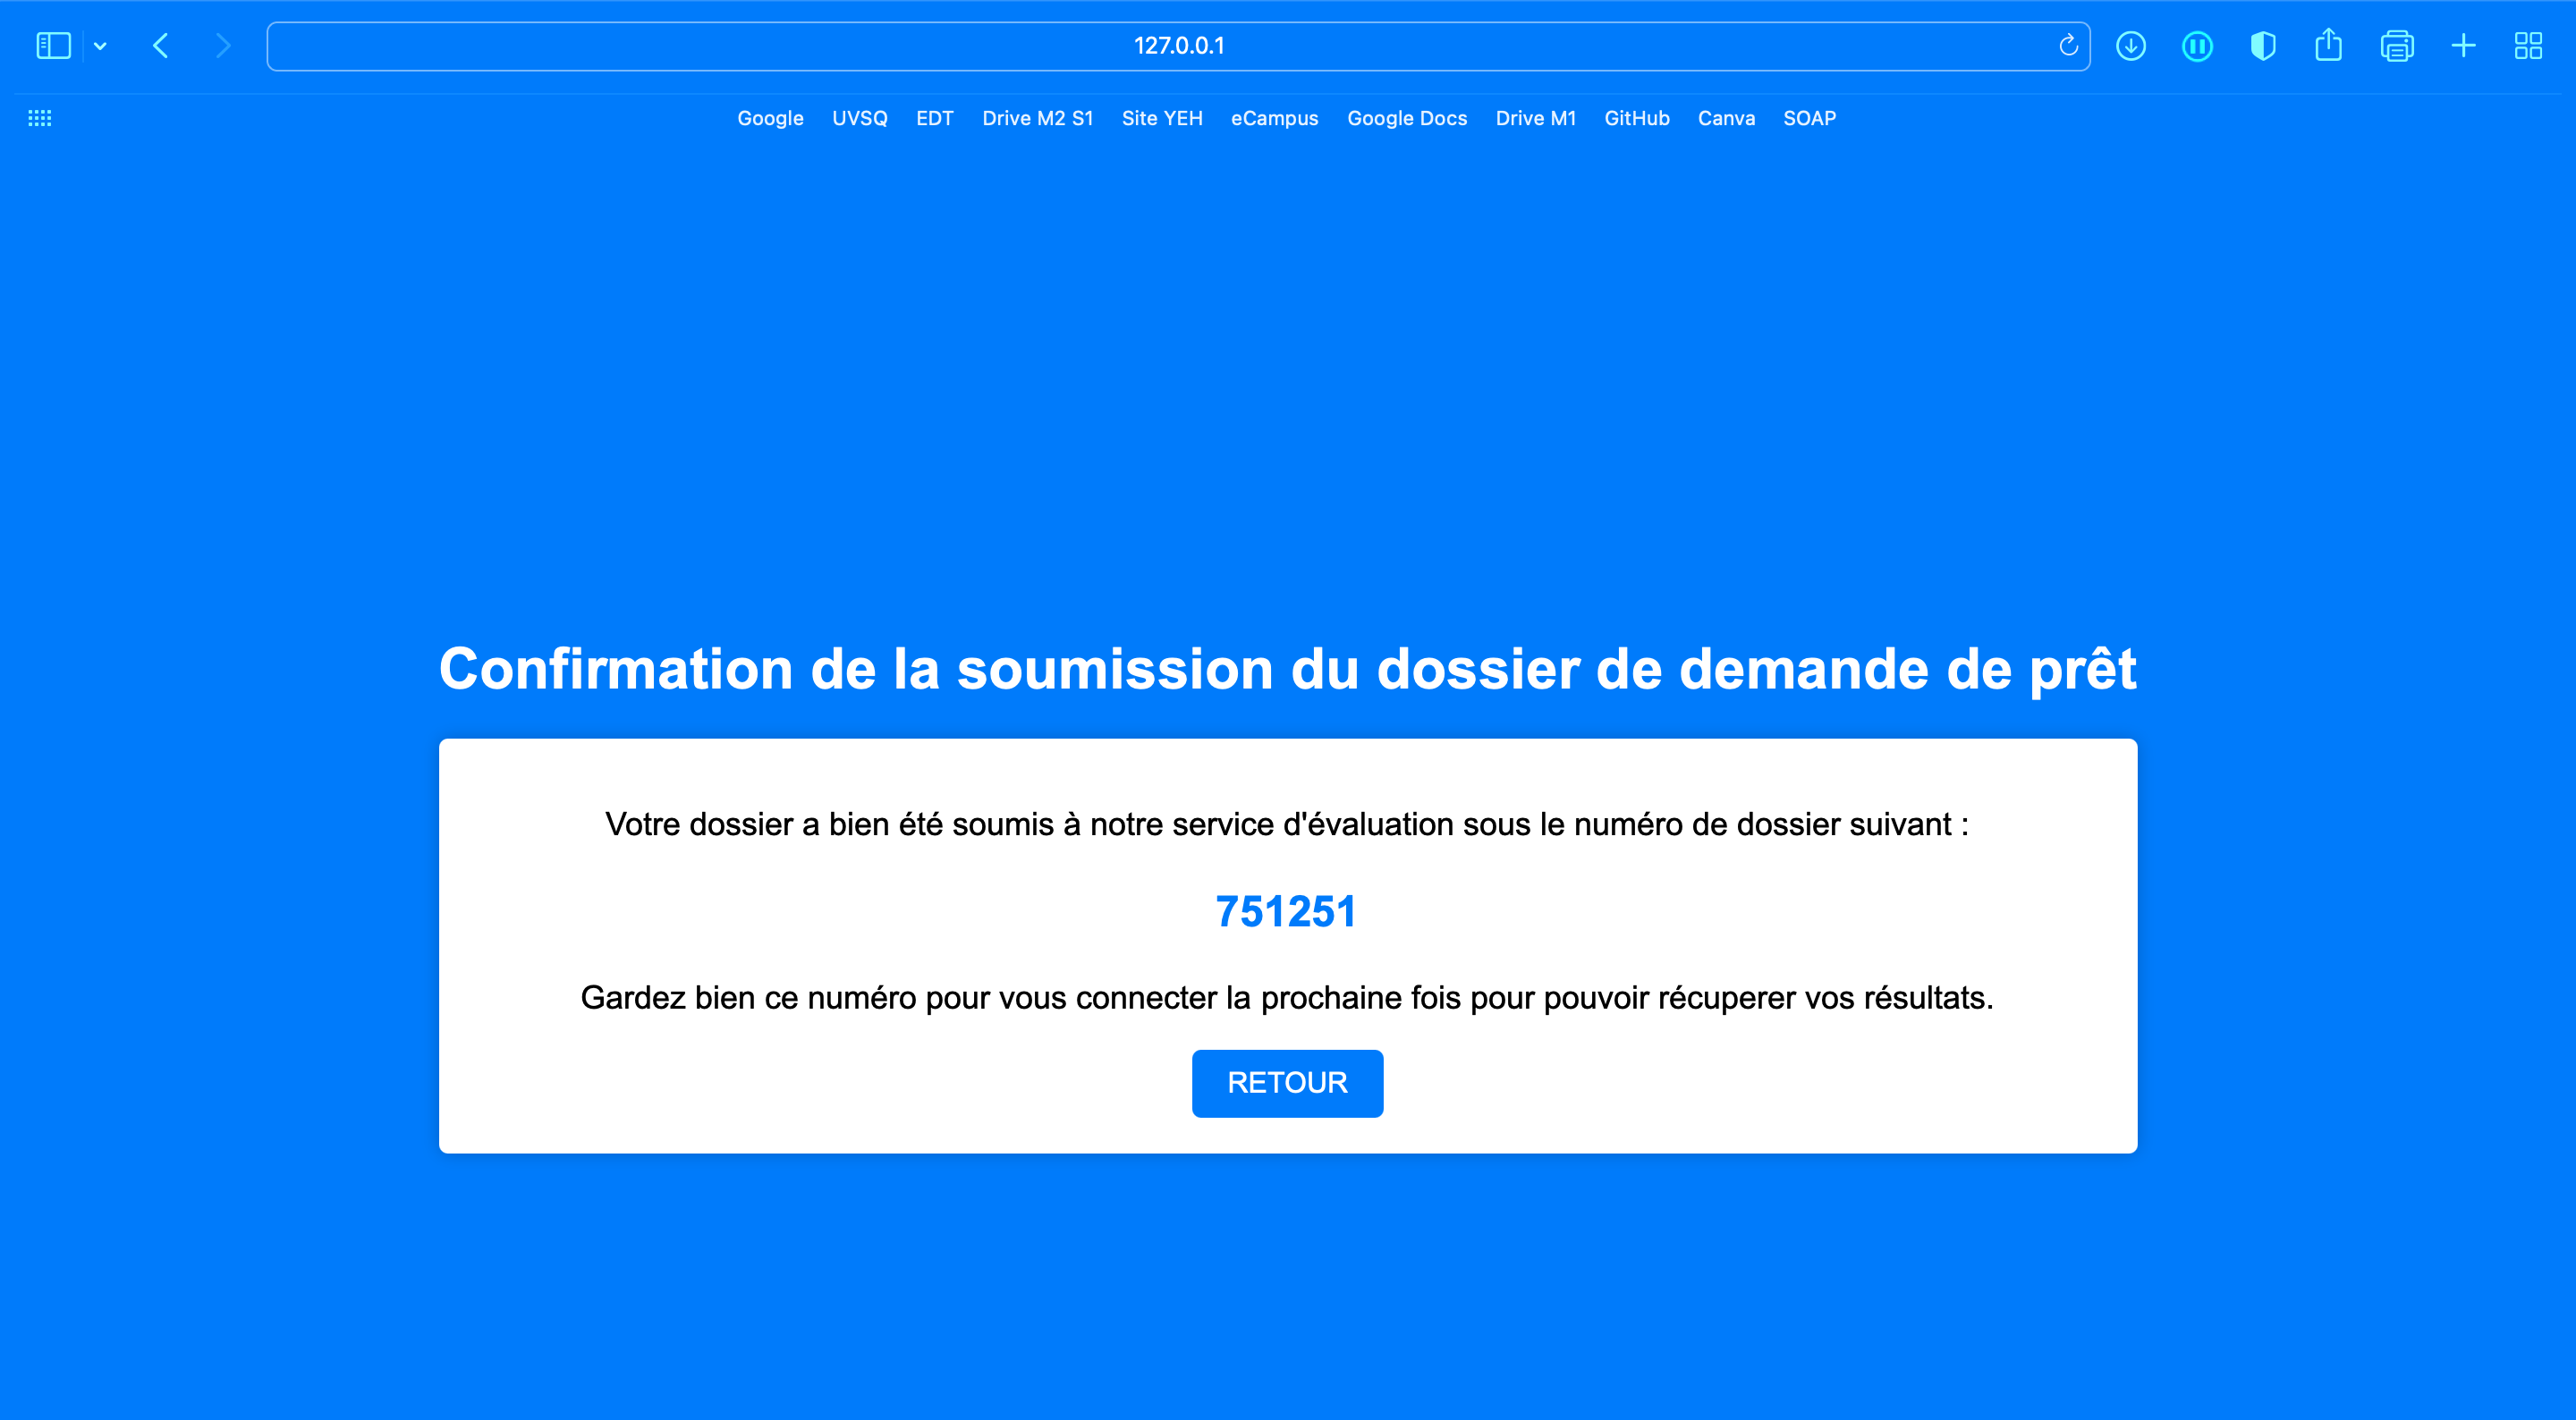
\includegraphics[width=\textwidth]{Images/8.1/confirmation.png}
    
    \subsubsection{Connexion : page de connexion pour consulter les résultats}
    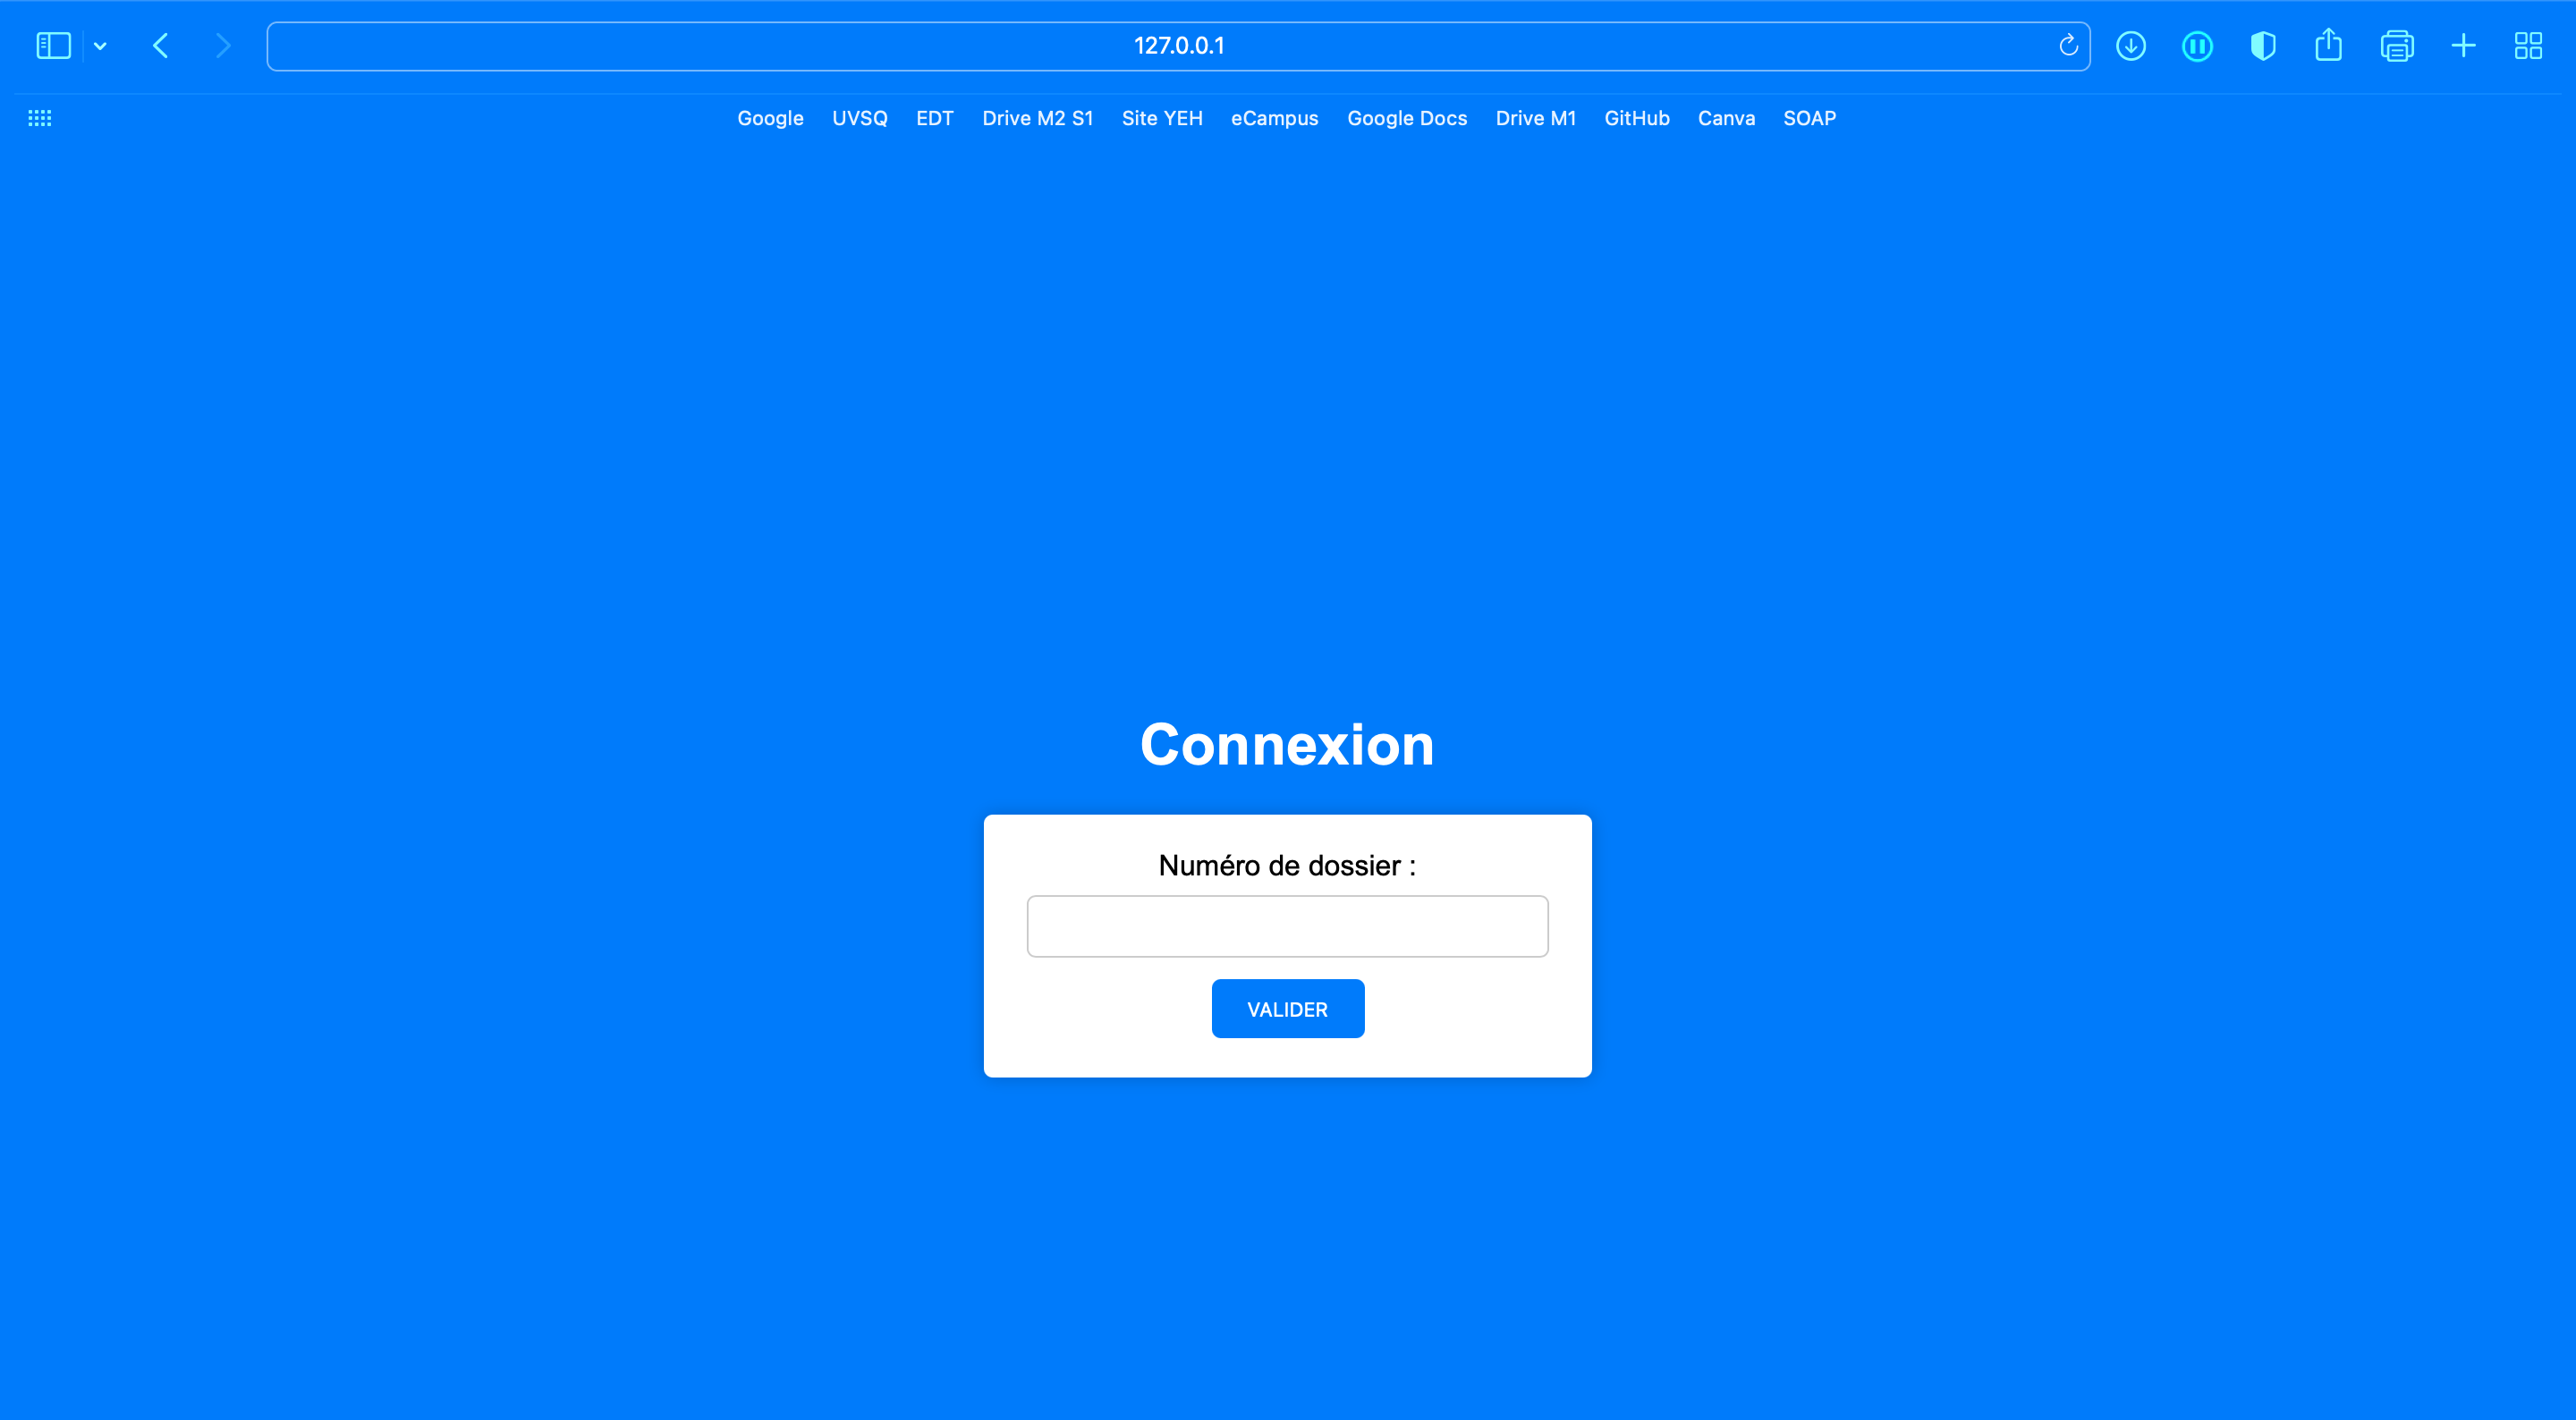
\includegraphics[width=\textwidth]{Images/8.1/connexion.png}
    
    \newpage
    
    \subsubsection{Disponible : page affichant que le résultat est disponible}
    \textbf{[Cas où l'évaluation de prêt a eu lieu]}\\ \\
    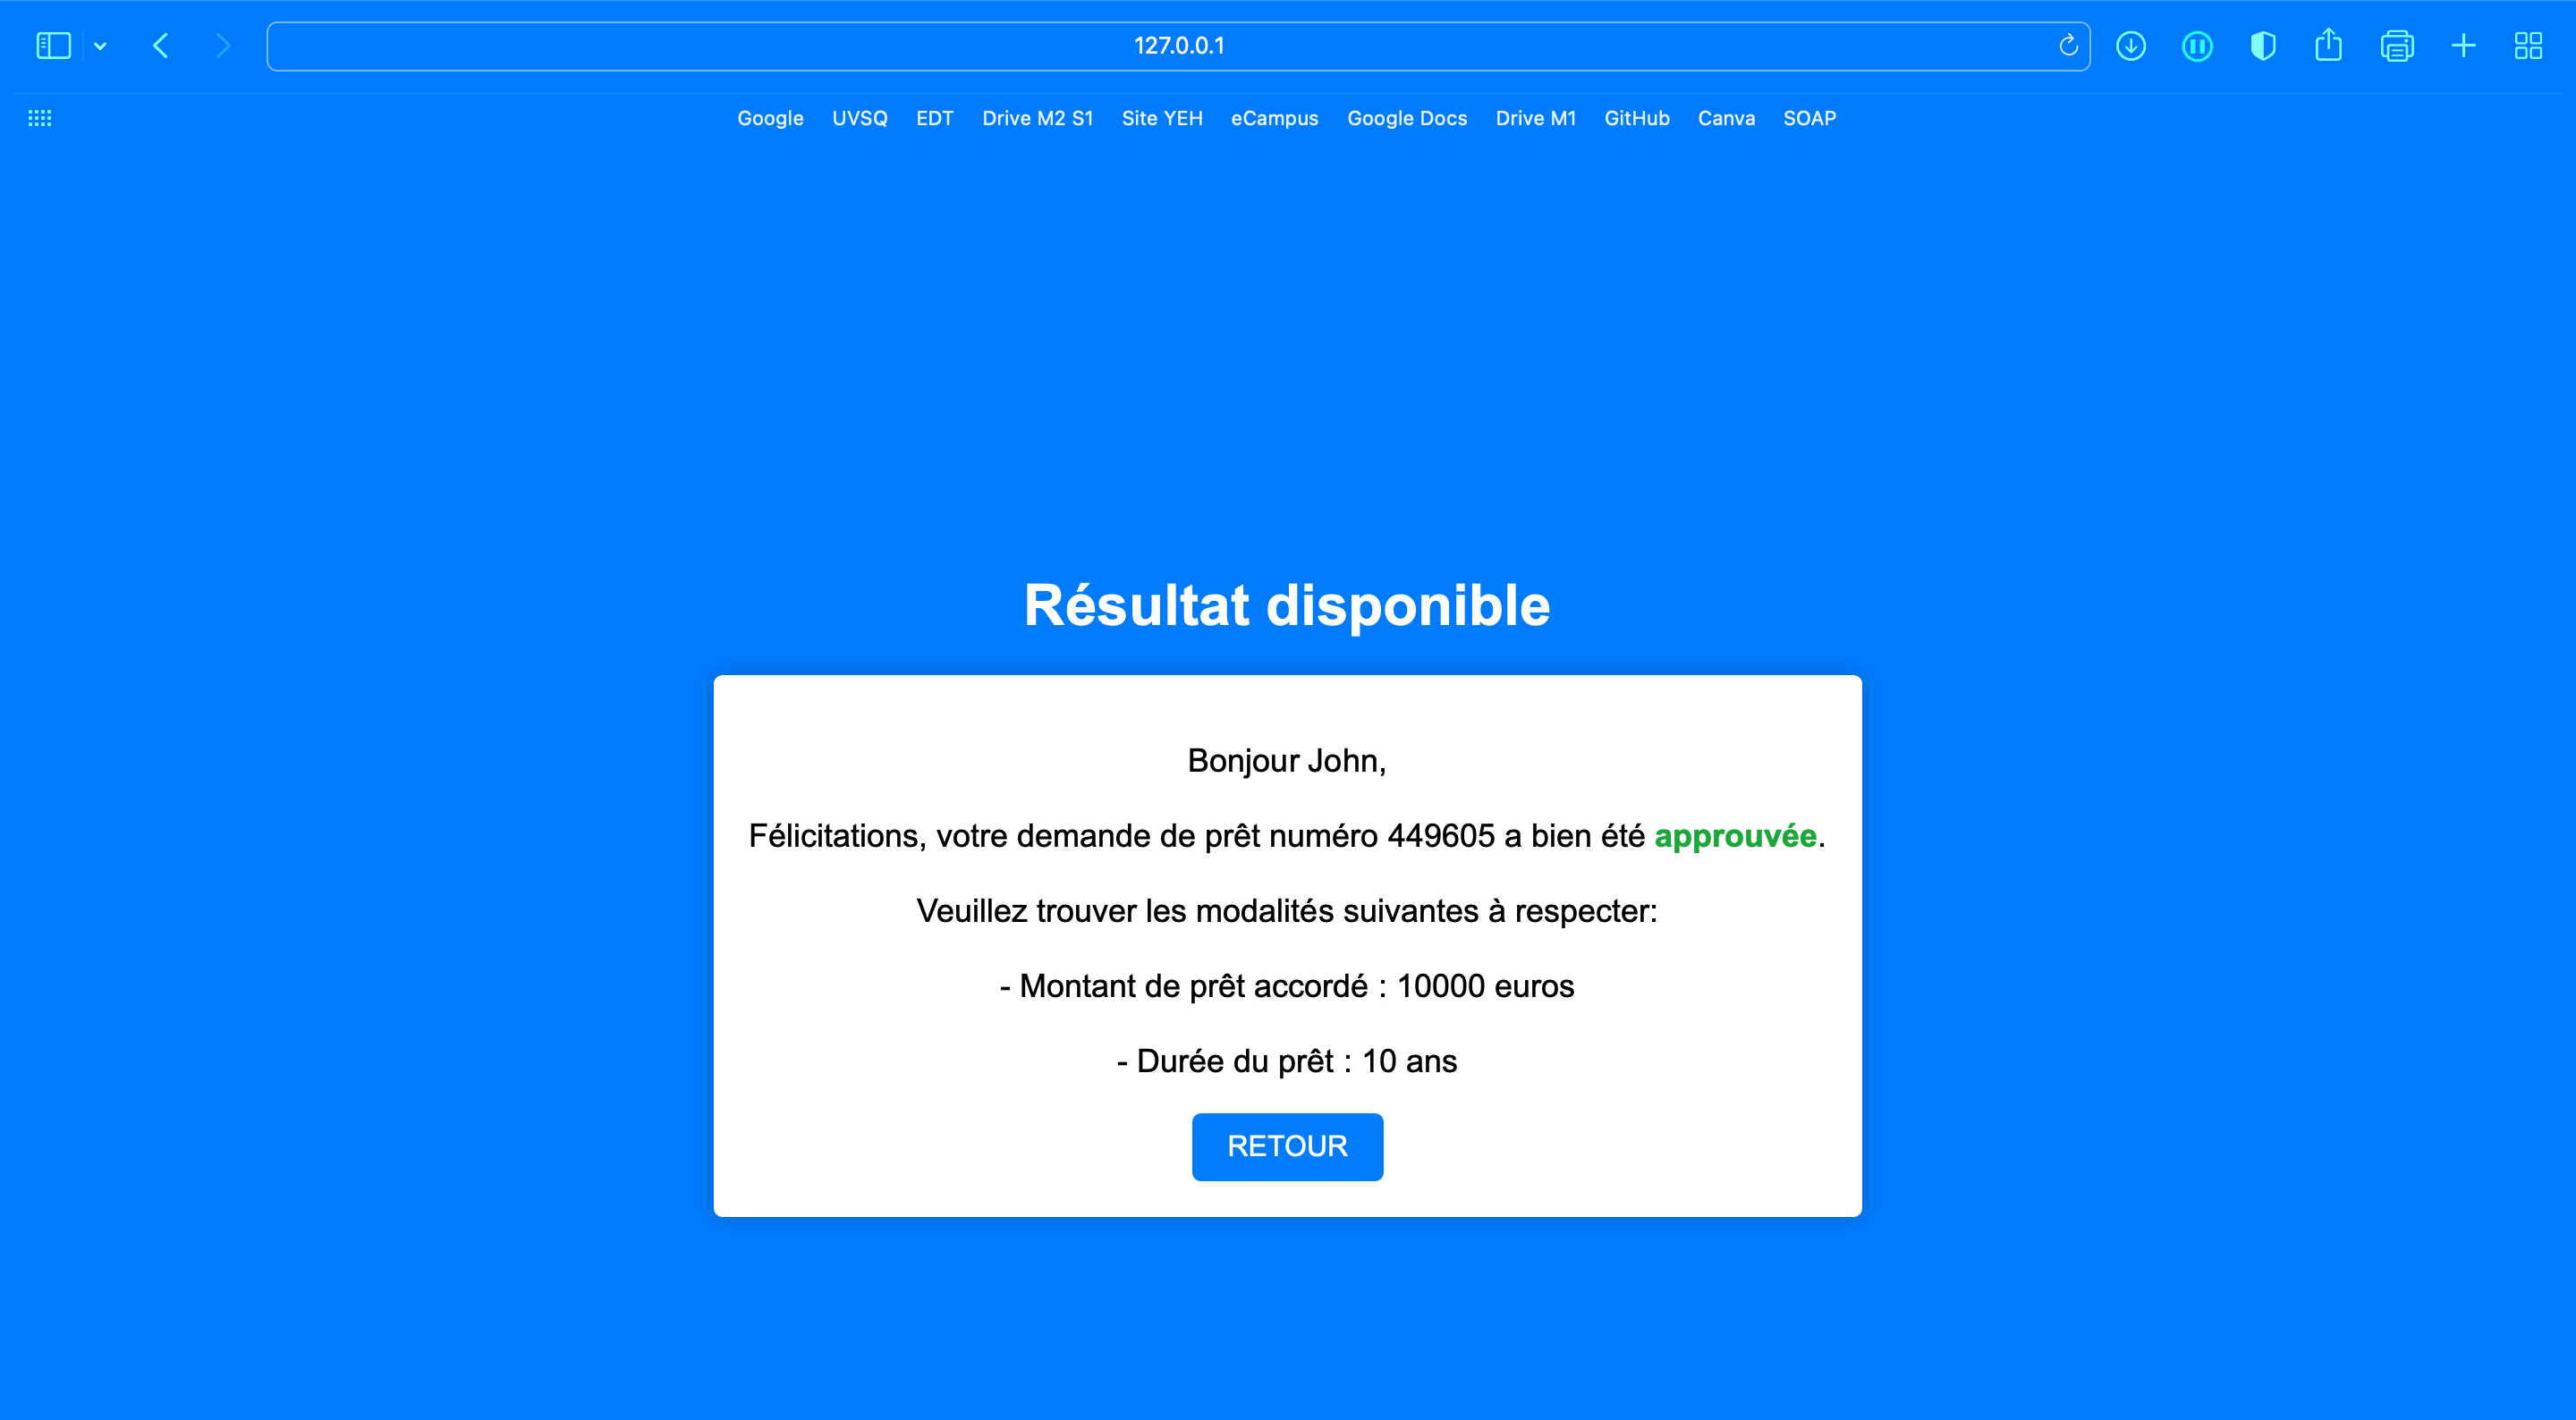
\includegraphics[width=\textwidth]{Images/8.1/disponible.png}

    \subsubsection{Introuvable : page affichant que le résultat est introuvable}
    \textbf{[Cas où l'évaluation de prêt n'a pas eu lieu car le numéro de dossier indiqué est inexistant]} \\ \\
    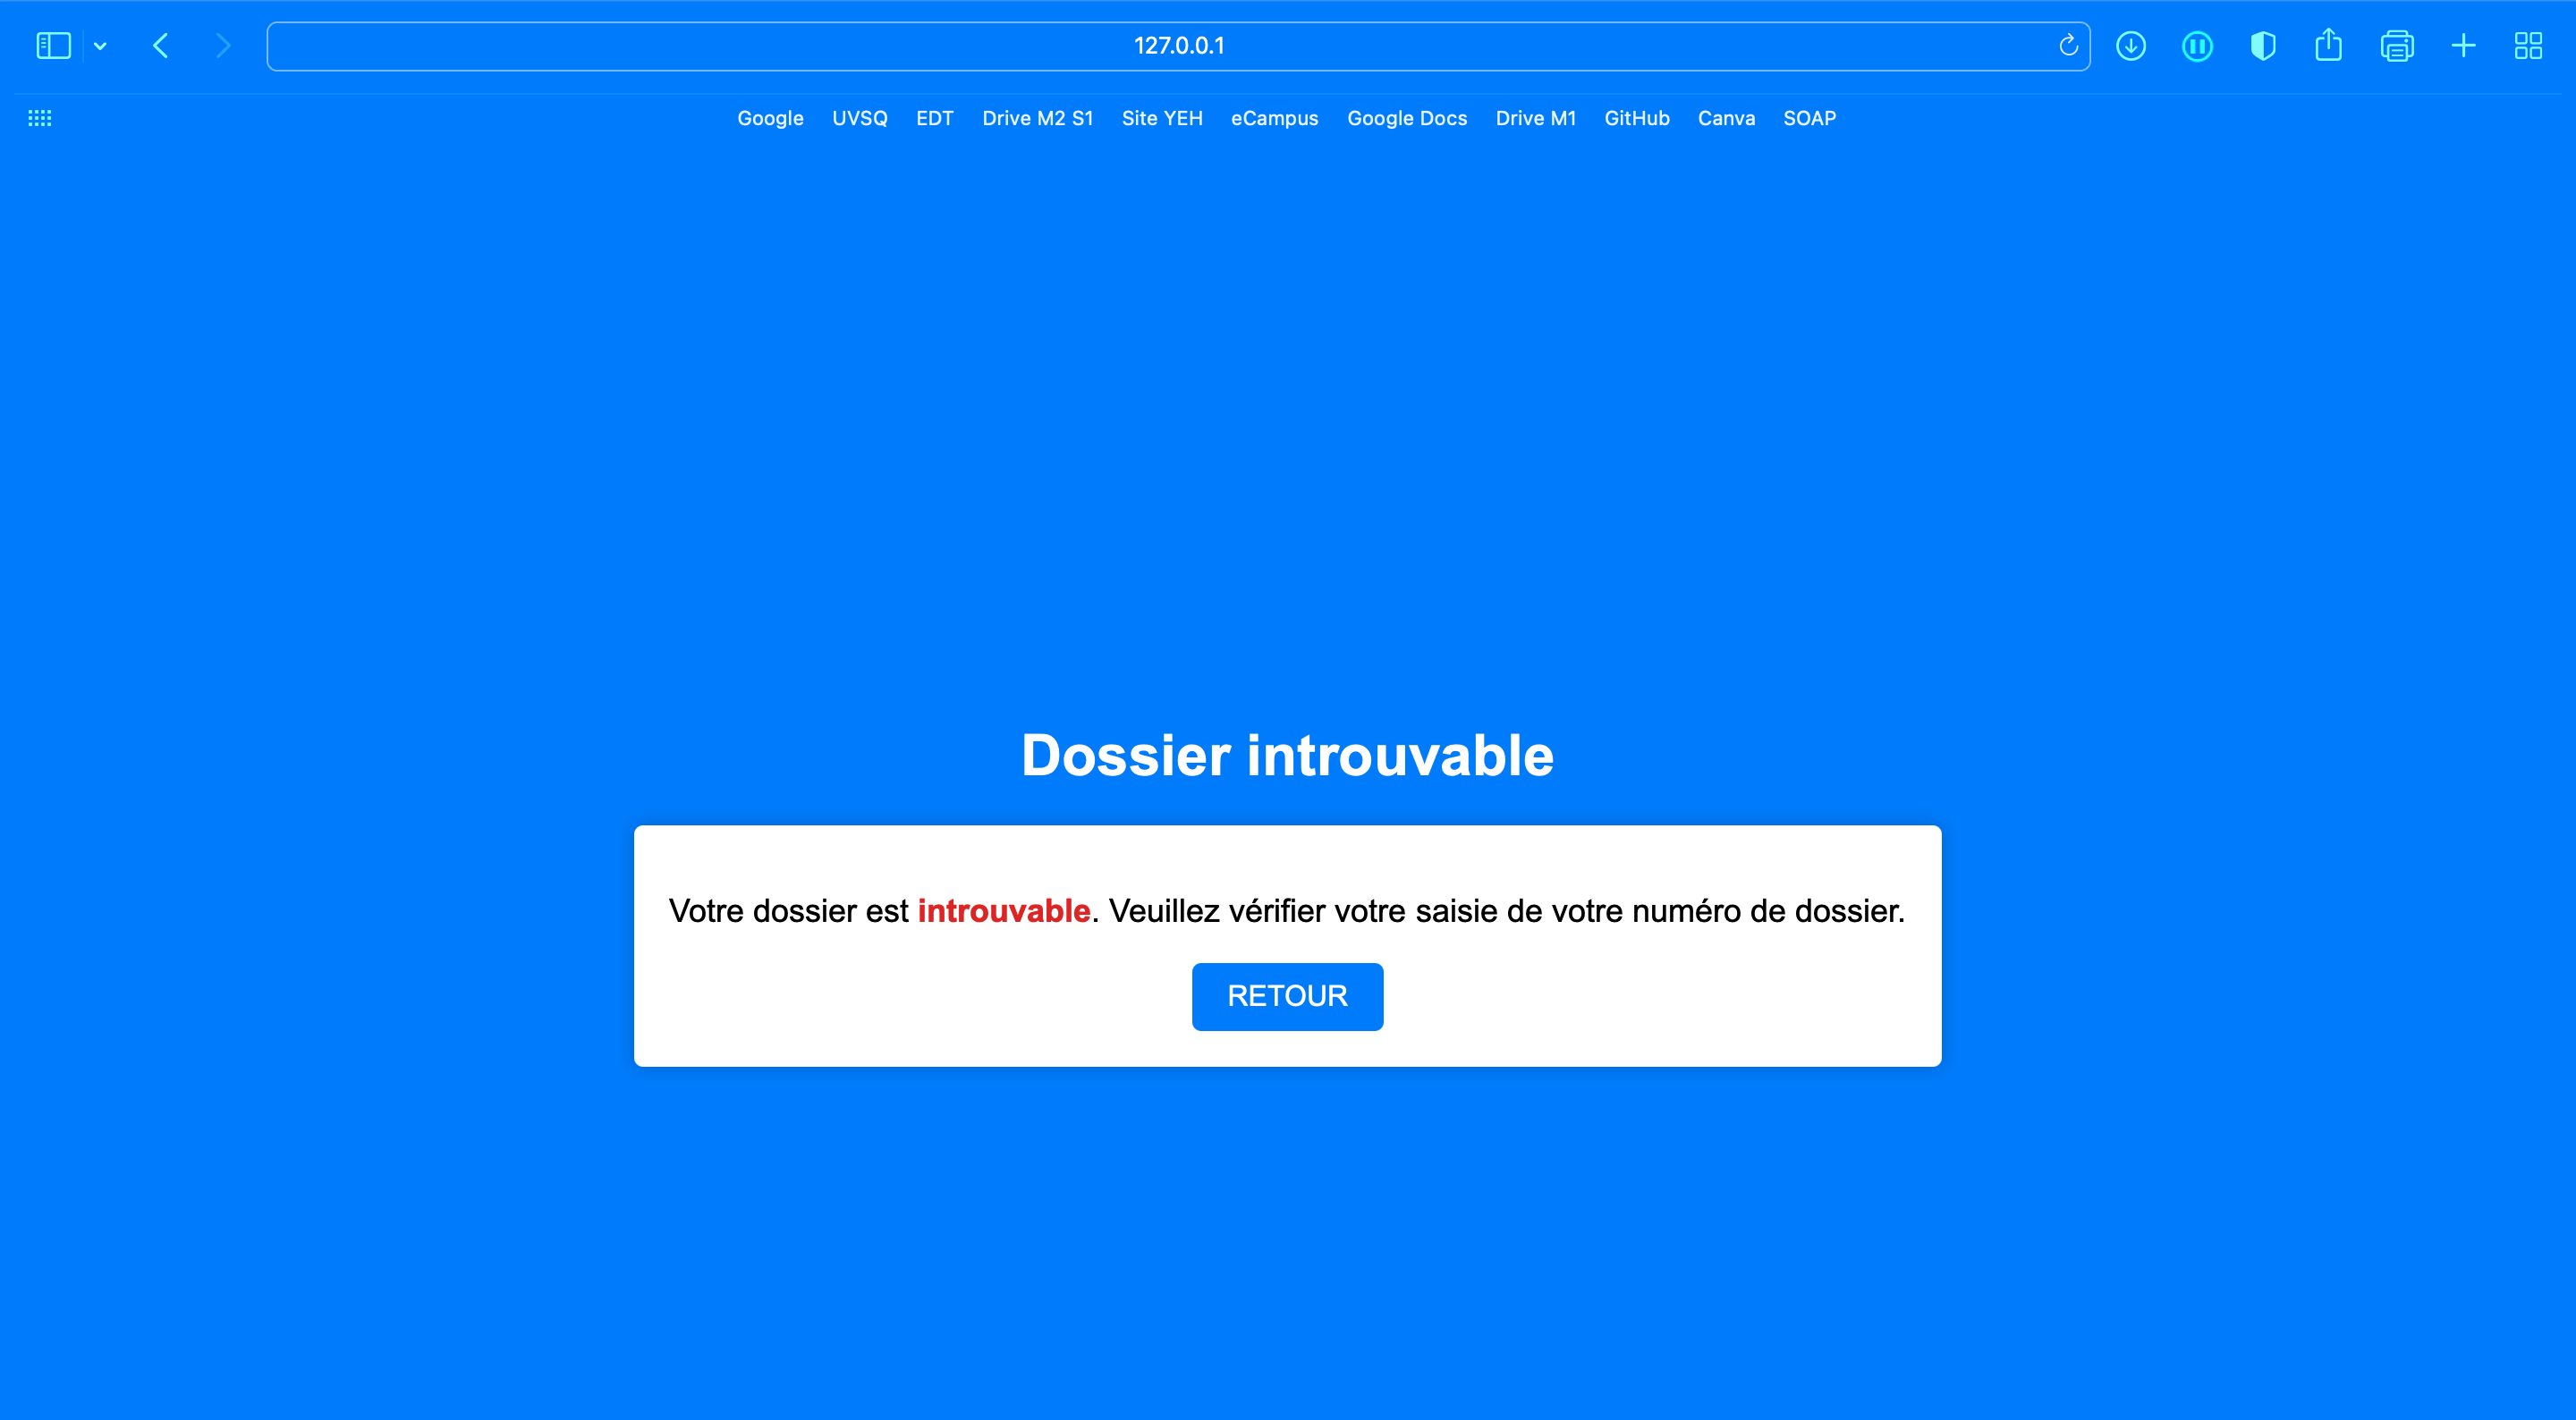
\includegraphics[width=\textwidth]{Images/8.1/introuvable.png}
    
    \newpage
    
    \subsubsection{Traitement : page affichant que le résultat n'est pas encore disponible}
    \textbf{[Cas où l'évaluation de prêt a eu lieu mais n'a pas aboutit car il y a eu un bug lors de l'évaluation de prêt]} \\ \\
    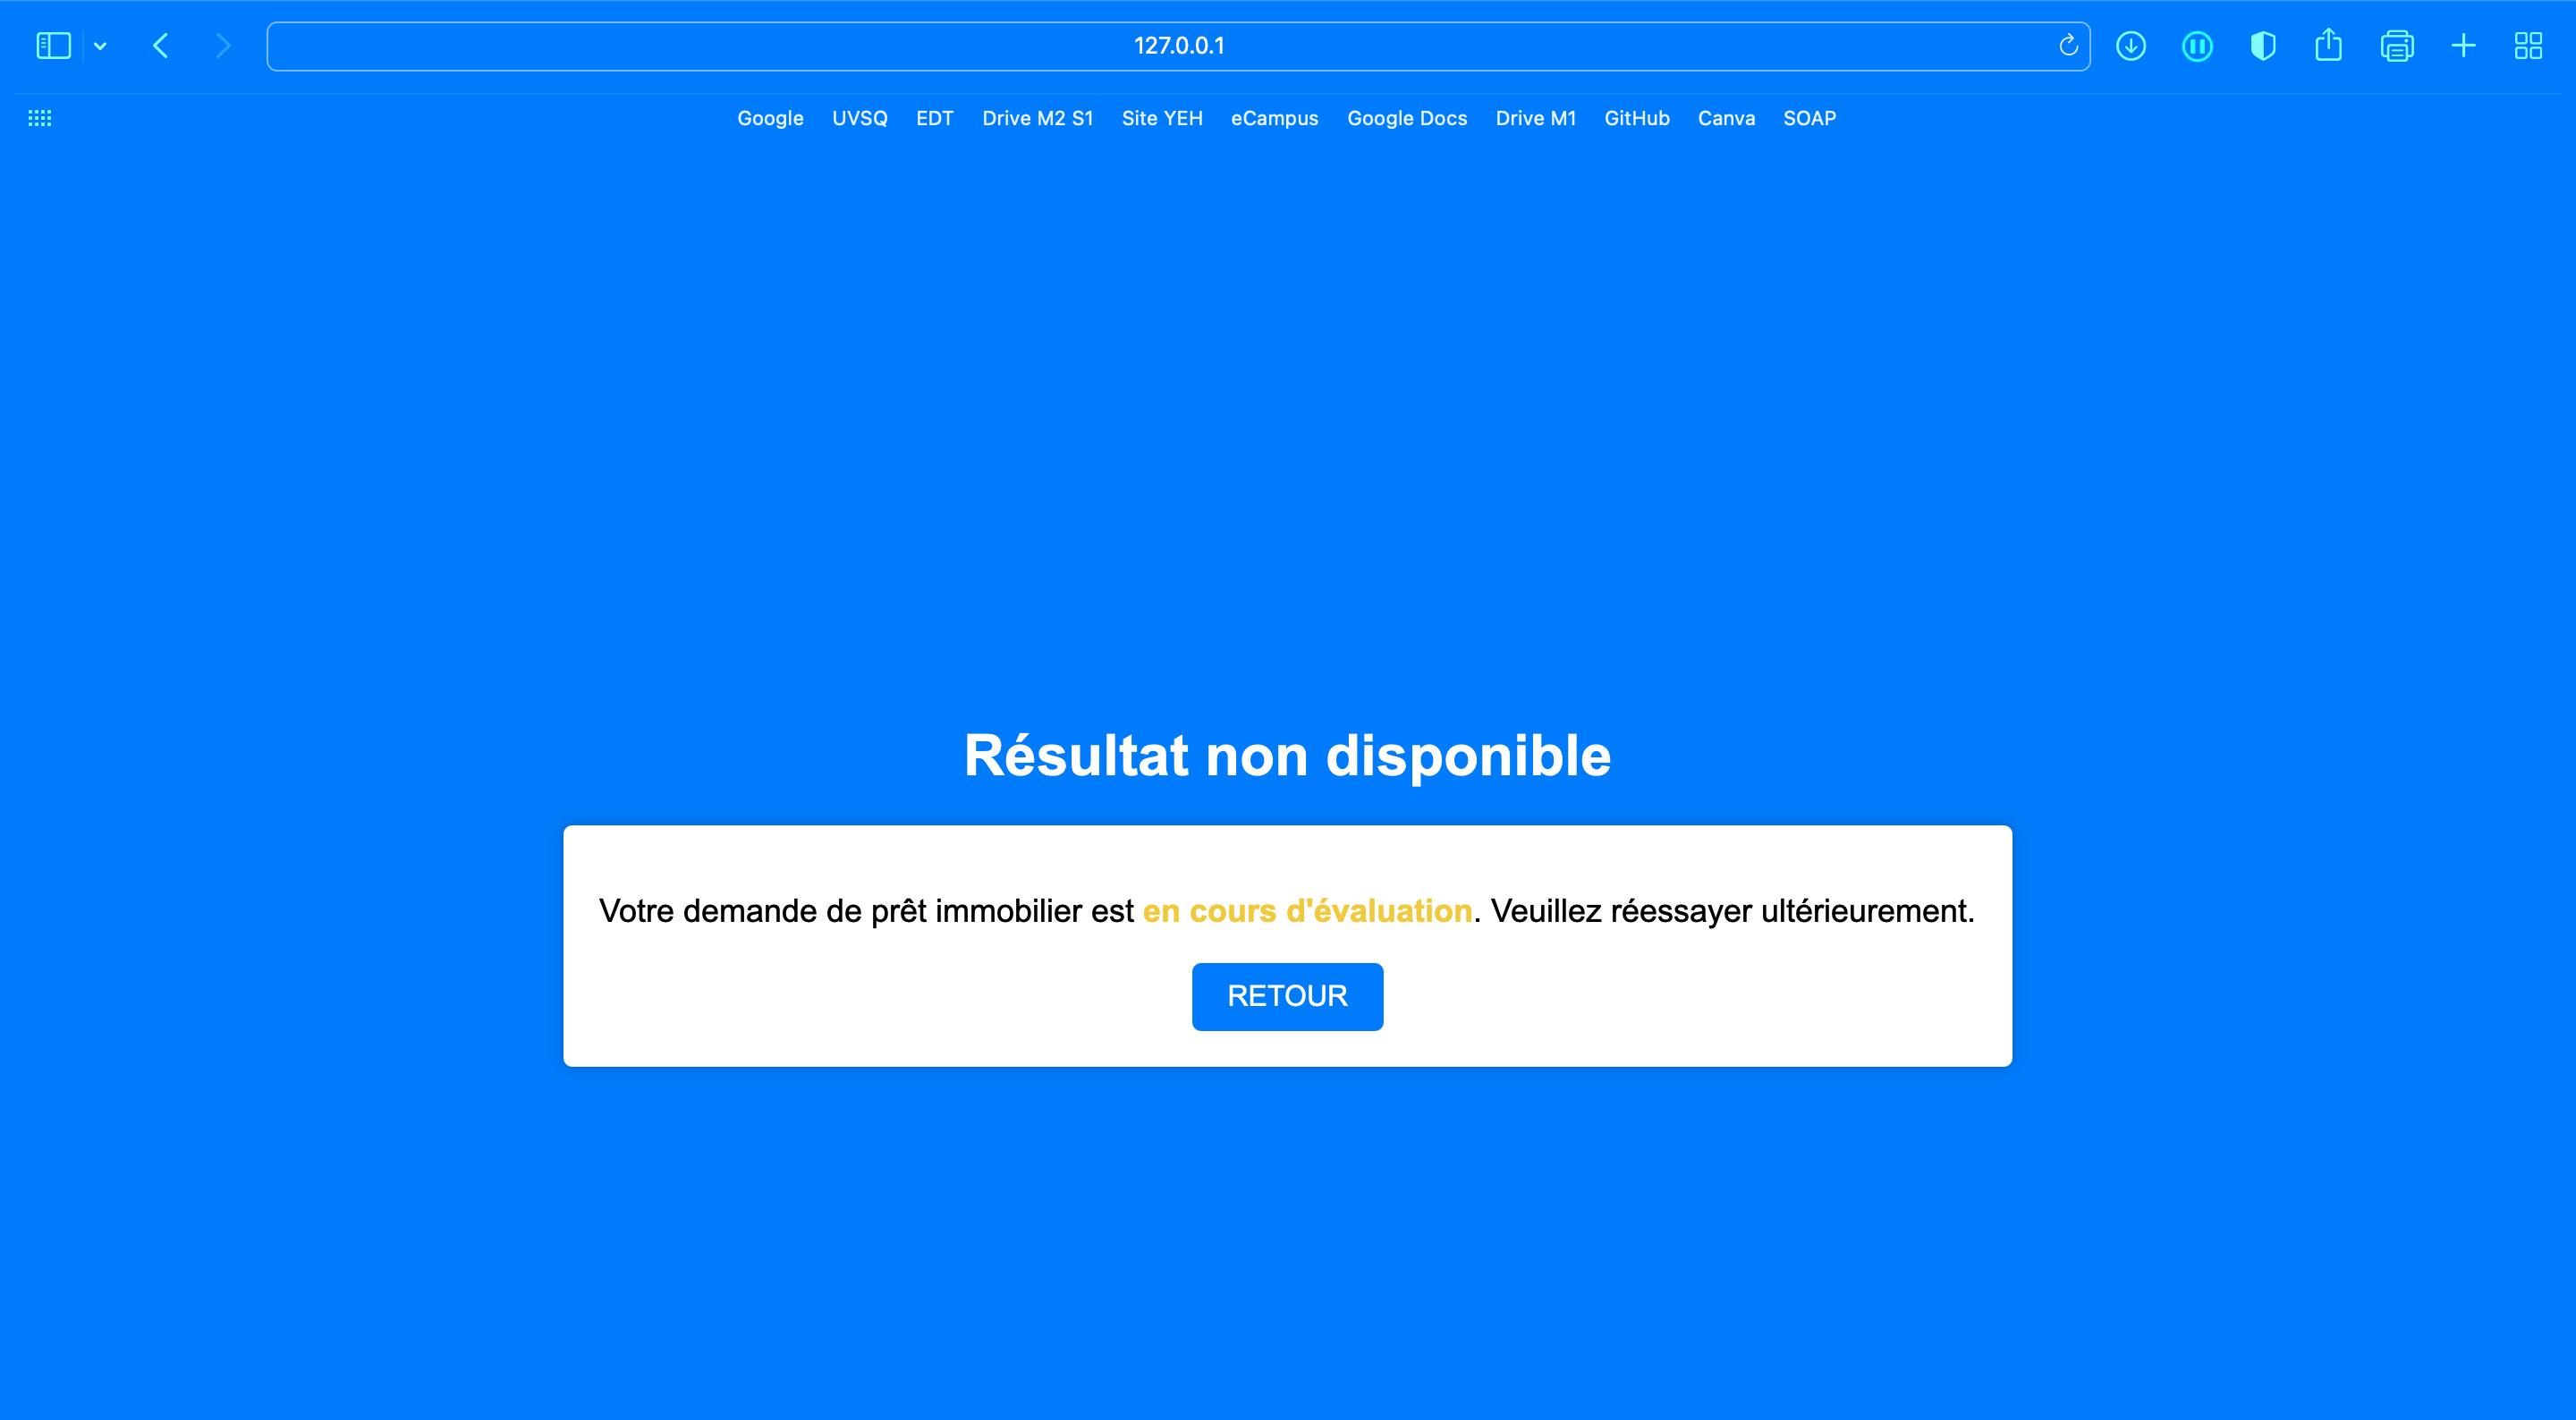
\includegraphics[width=\textwidth]{Images/8.1/traitement.png}
    
    \subsection{Lancement de l'application}
    \subsubsection{Commandes}
Voici les étapes à suivre afin de pouvoir exécuter l'application:
\begin{itemize}
    \item Configuration de l'environnement virtuel \texttt{venv} et ajout des dépendances nécessaires : \\
    \texttt{chmod 774 ./configure} puis \texttt{./configure}
    \item Lancement du serveur web : \texttt{chmod 774 ./run} puis \texttt{./run}
    \item Disponibilité de l'interface : \texttt{http://localhost:8000}
\end{itemize}

    \subsubsection{Côté Client : Web}
    En lançant l'application, le client arrive sur \texttt{http://localhost:8000} qui est la page d'accueil (voir 8.1.1). \\
    Il a le choix entre "Déposer un dossier" et "Voir le Résultat". 
    
    \newpage
    
    \underline{Cas 1 : DEPOT D'UN DOSSIER} \\ \\
    Si il clique sur "Déposer un dossier", il est redirigé vers la page de formulaire. Il remplit le formulaire comme ceci:
    \\ \\
		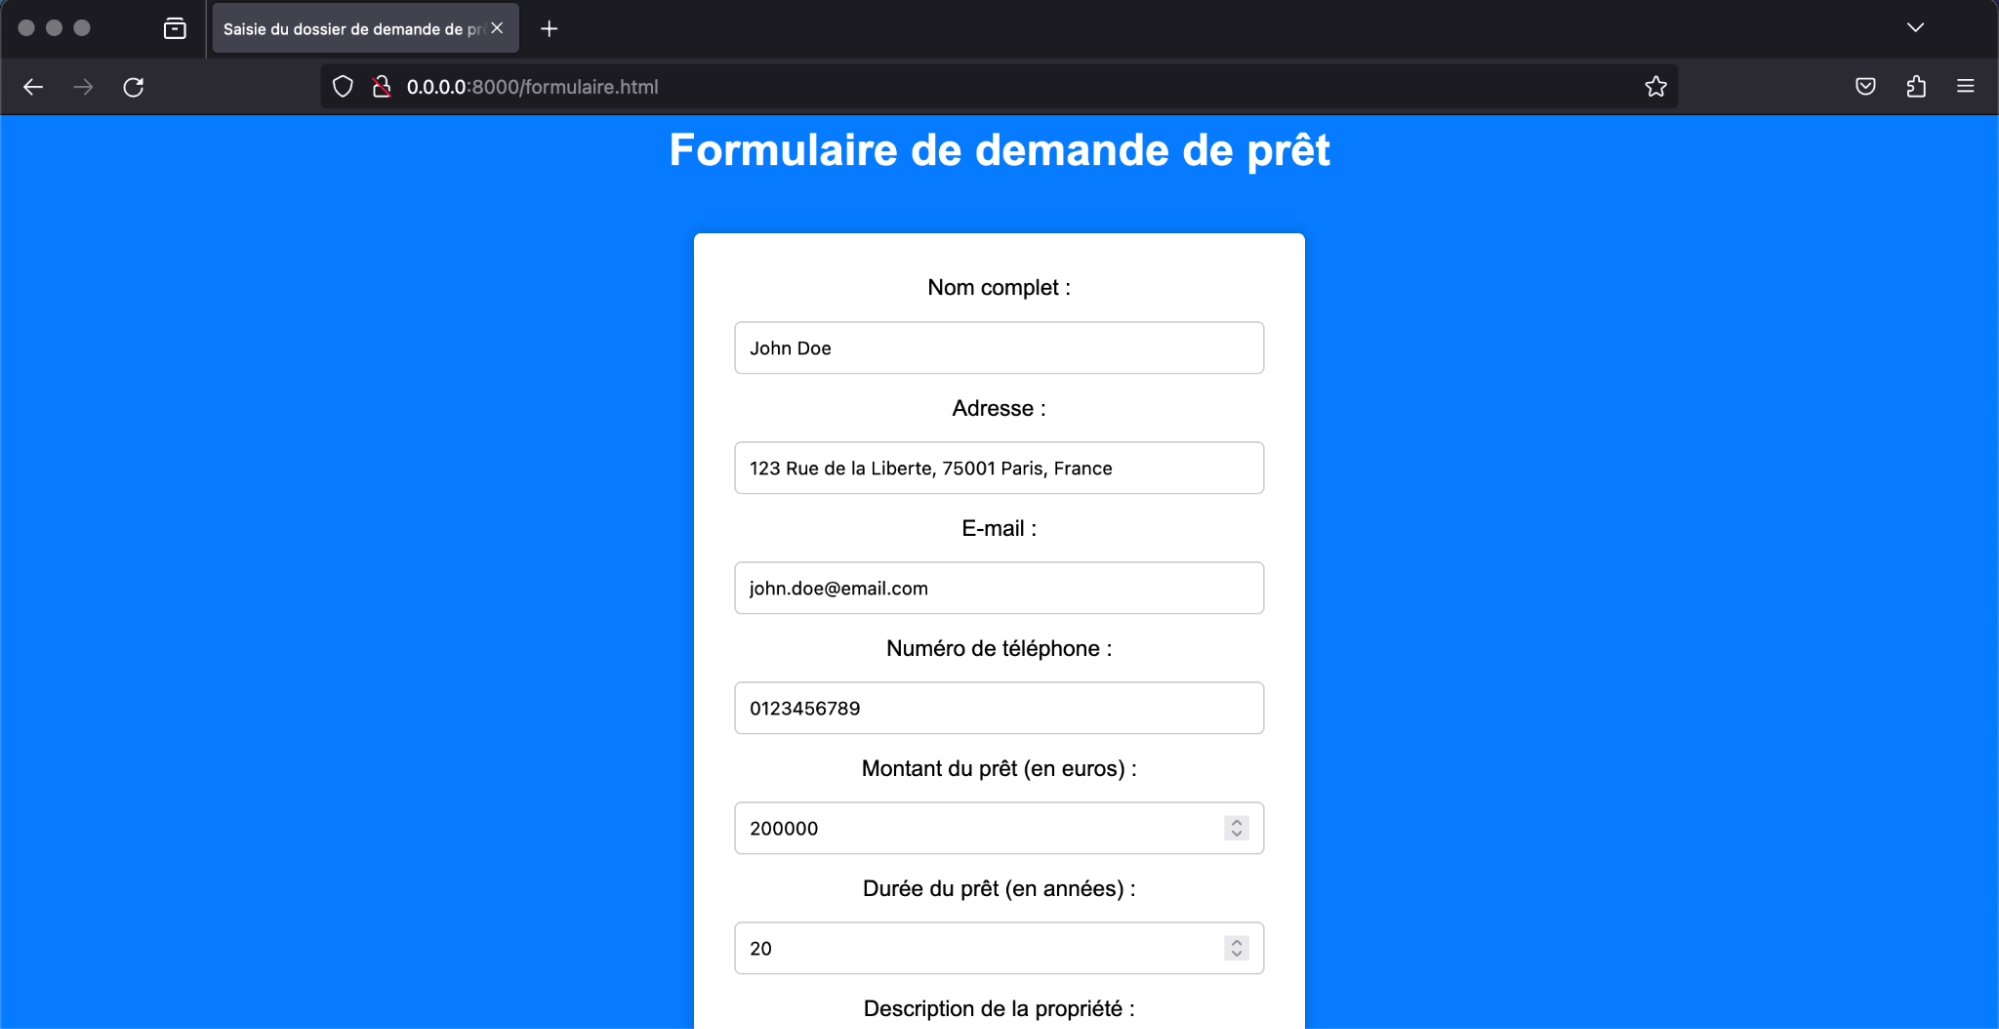
\includegraphics[width=\textwidth]{Images/8.2/formulairea1.png} \\
		
\includegraphics[width=\textwidth]{Images/8.2/formulairea2.png} \\
     Après avoir cliqué sur le bouton "Soumettre", la page de confirmation s’ouvre comme ceci:
        \\
		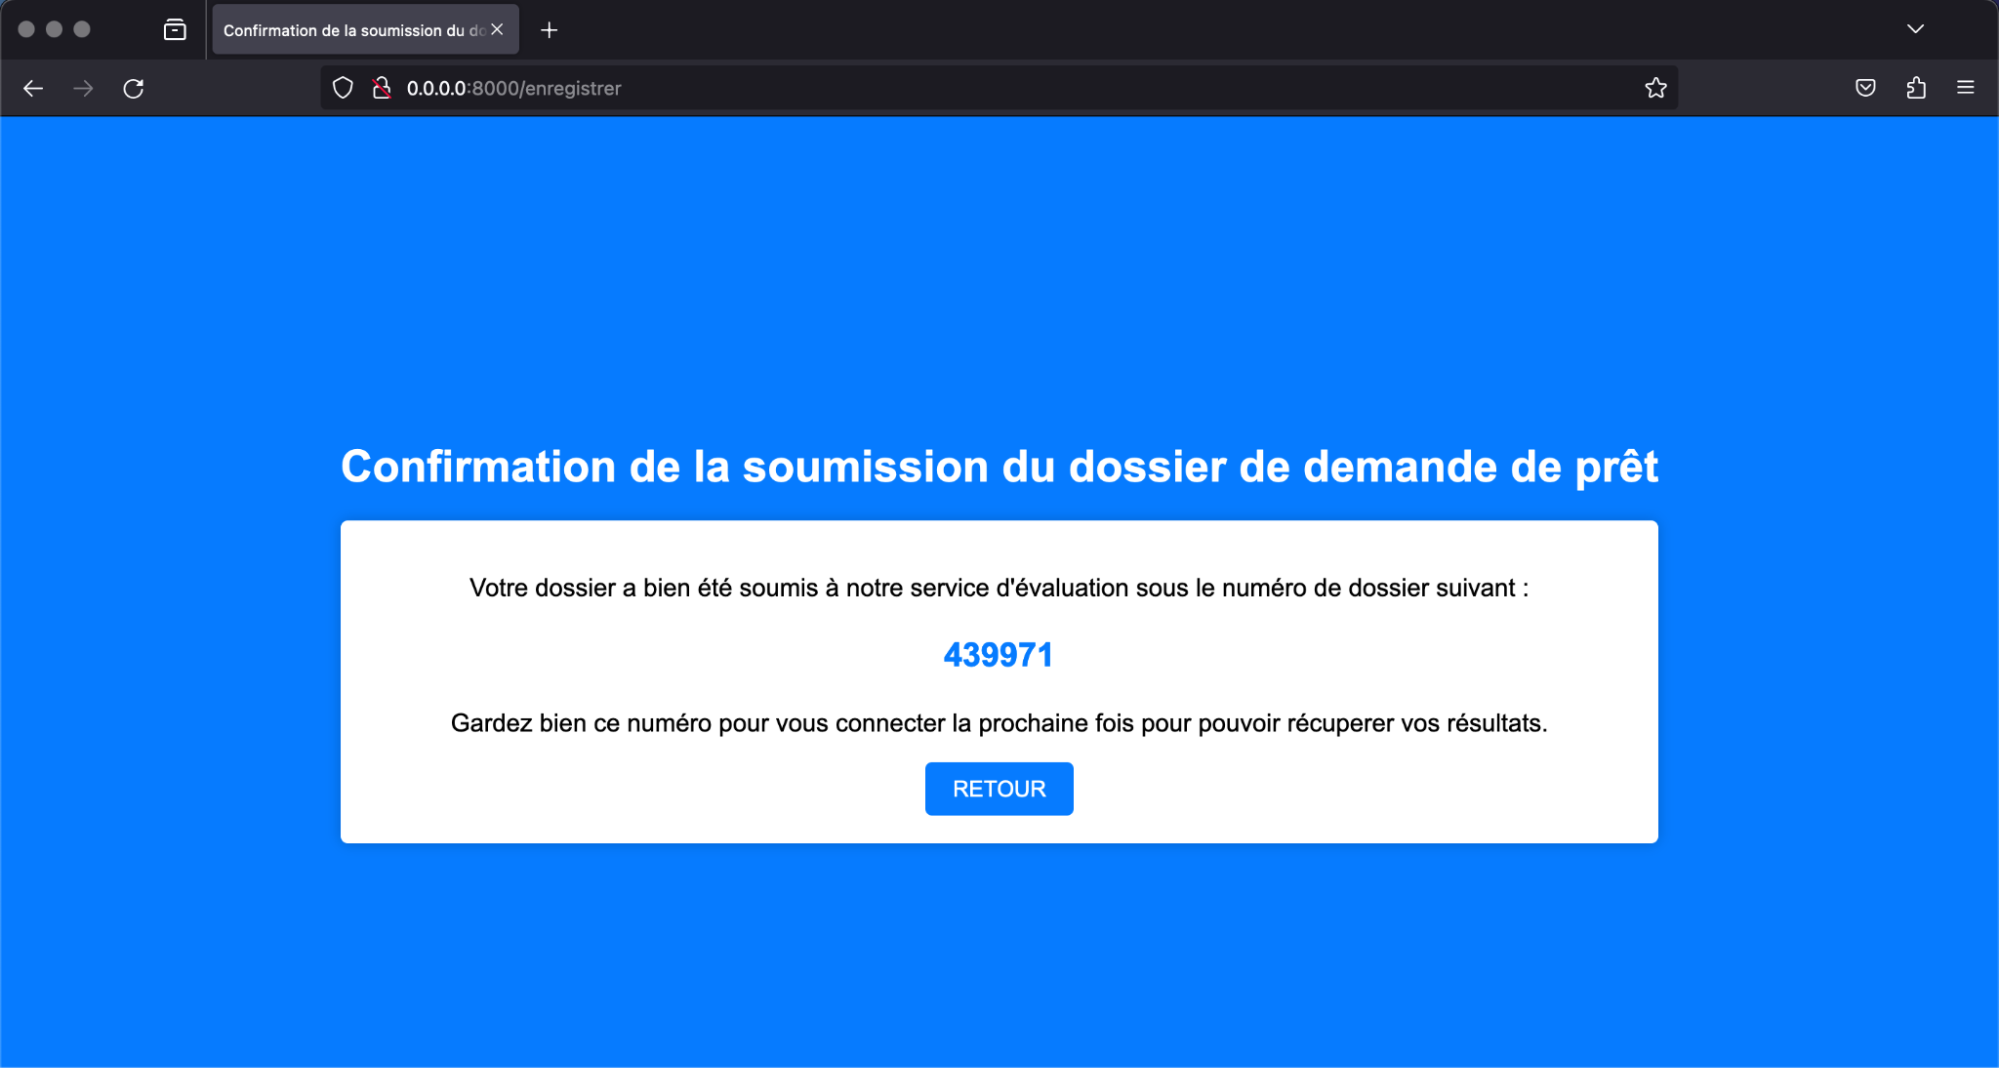
\includegraphics[width=\textwidth]{Images/8.2/depota.png} \\
		\\
    Elle nous indique le numéro de dossier de la demande qui est à conserver pour pouvoir consulter les résultats par la suite. Si l'utilisateur clique sur "Retour", il revient à la page d'accueil \\ \\

    \underline{Cas 2 : VISUALISATION DU RESULTAT} \\ \\
	Si il clique sur le bouton "Voir le résultat", la page de connexion s'affiche \\
		\\
	   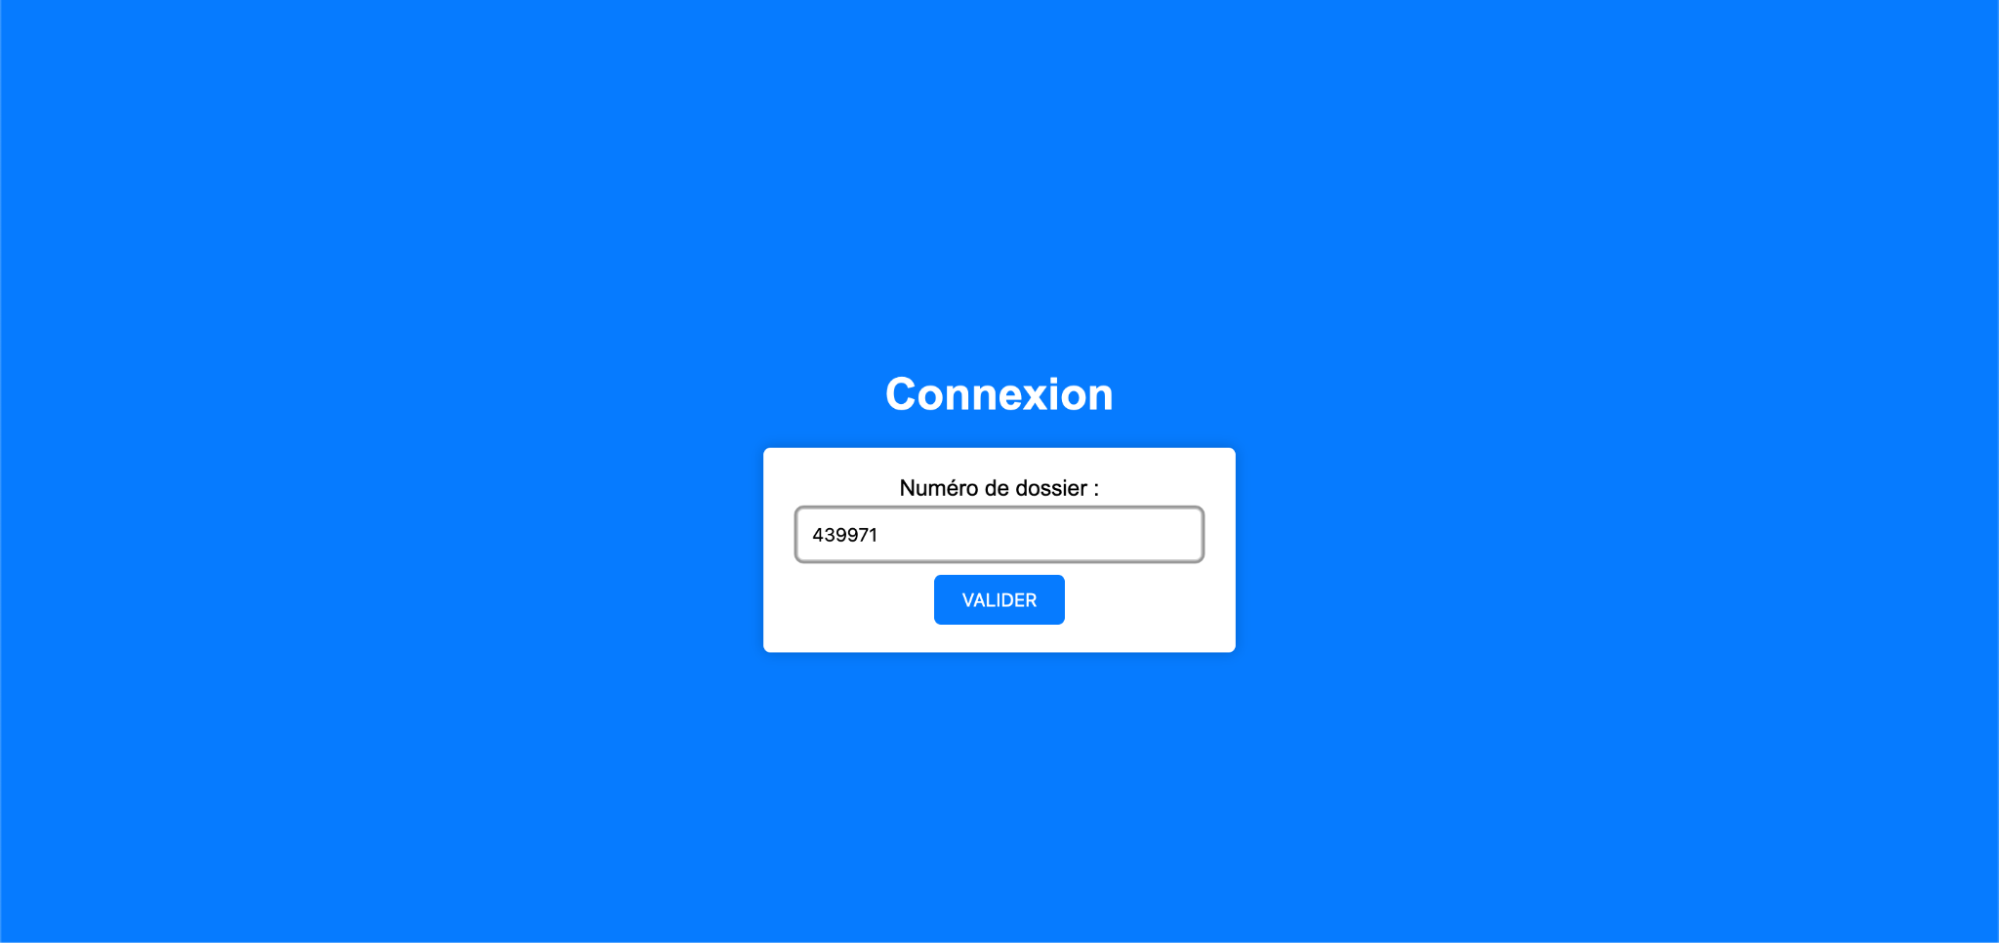
\includegraphics[width=\textwidth]{Images/8.2/connexiona.png}  \\
	   \\
	L'utilisateur saisit donc son numéro de dossier qu'il a copié lors de la confirmation de la soumission du formulaire.
    L'utilisateur accède à la page de résultat. \\
    
    Voici un exemple lorsque le dossier est accepté, on trouve les modalités à respecter : \\
	   \\
	   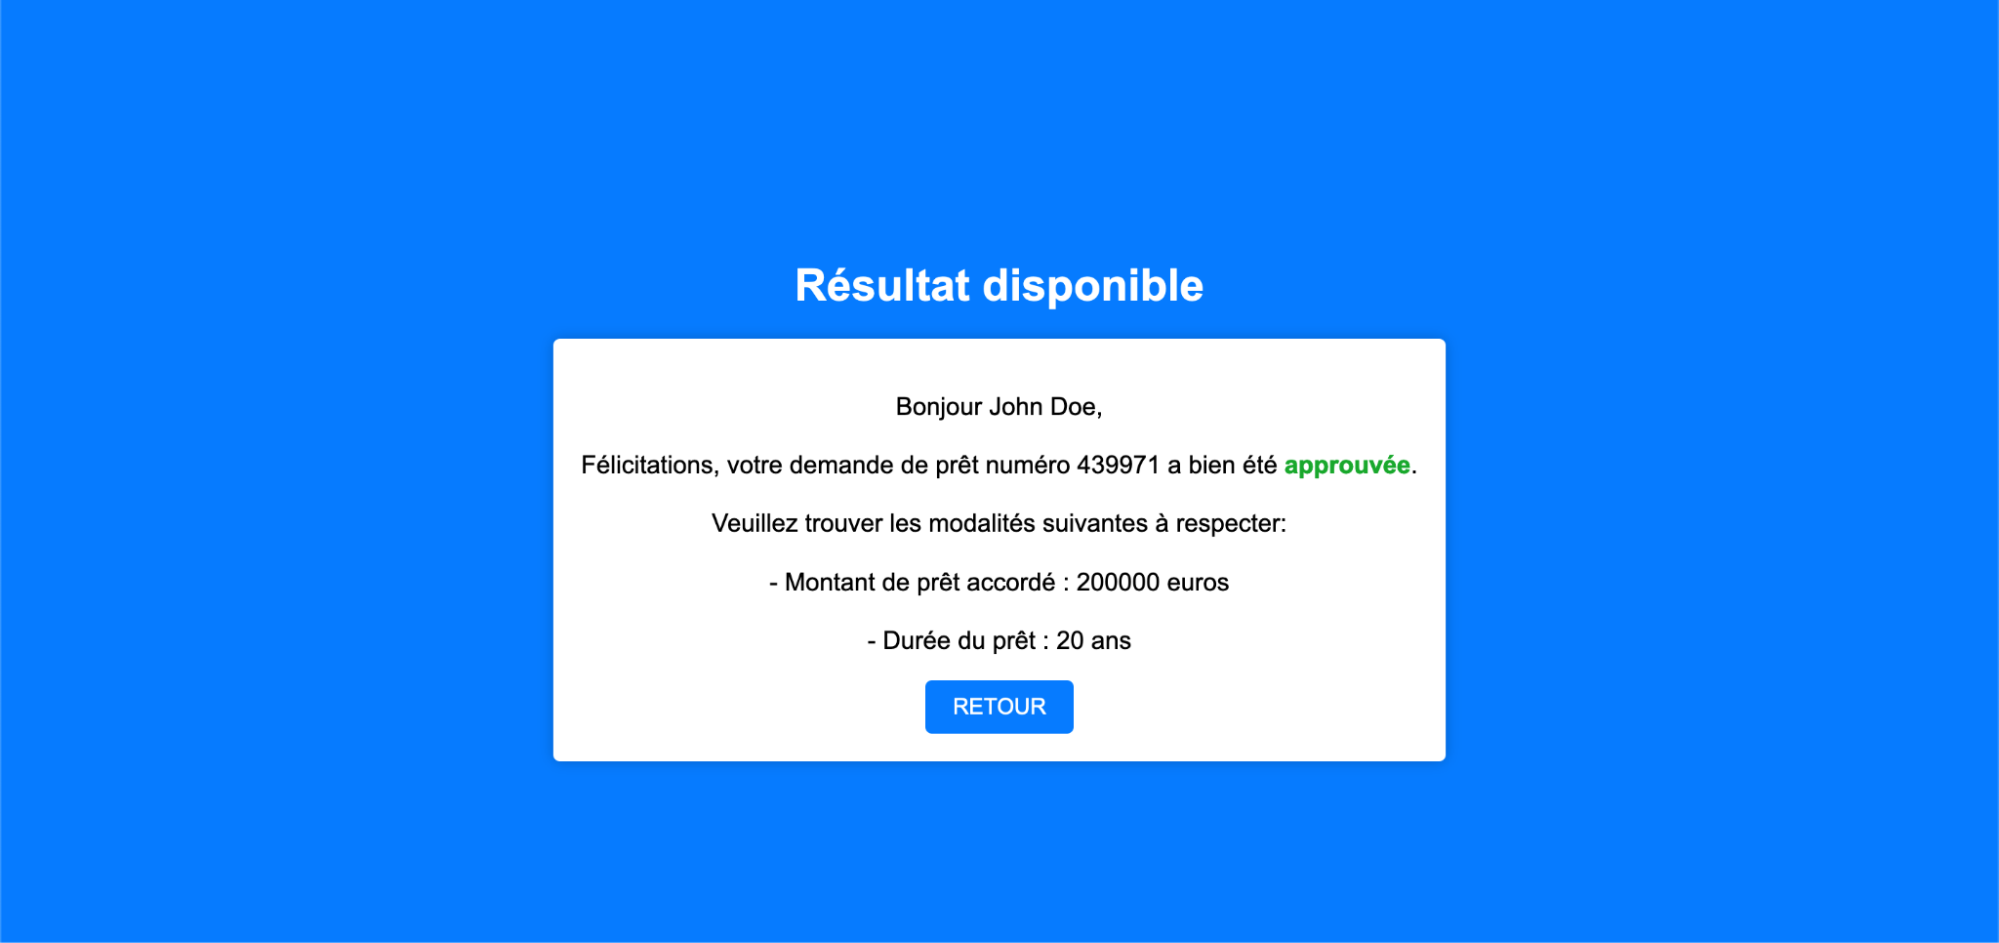
\includegraphics[width=\textwidth]{Images/8.2/confirmationa.png} \\
	   \\
	   
	   \newpage
	   
	Voici un exemple lorsque le dossier est refusé, on trouve les raisons du refus : \\
	   \\
    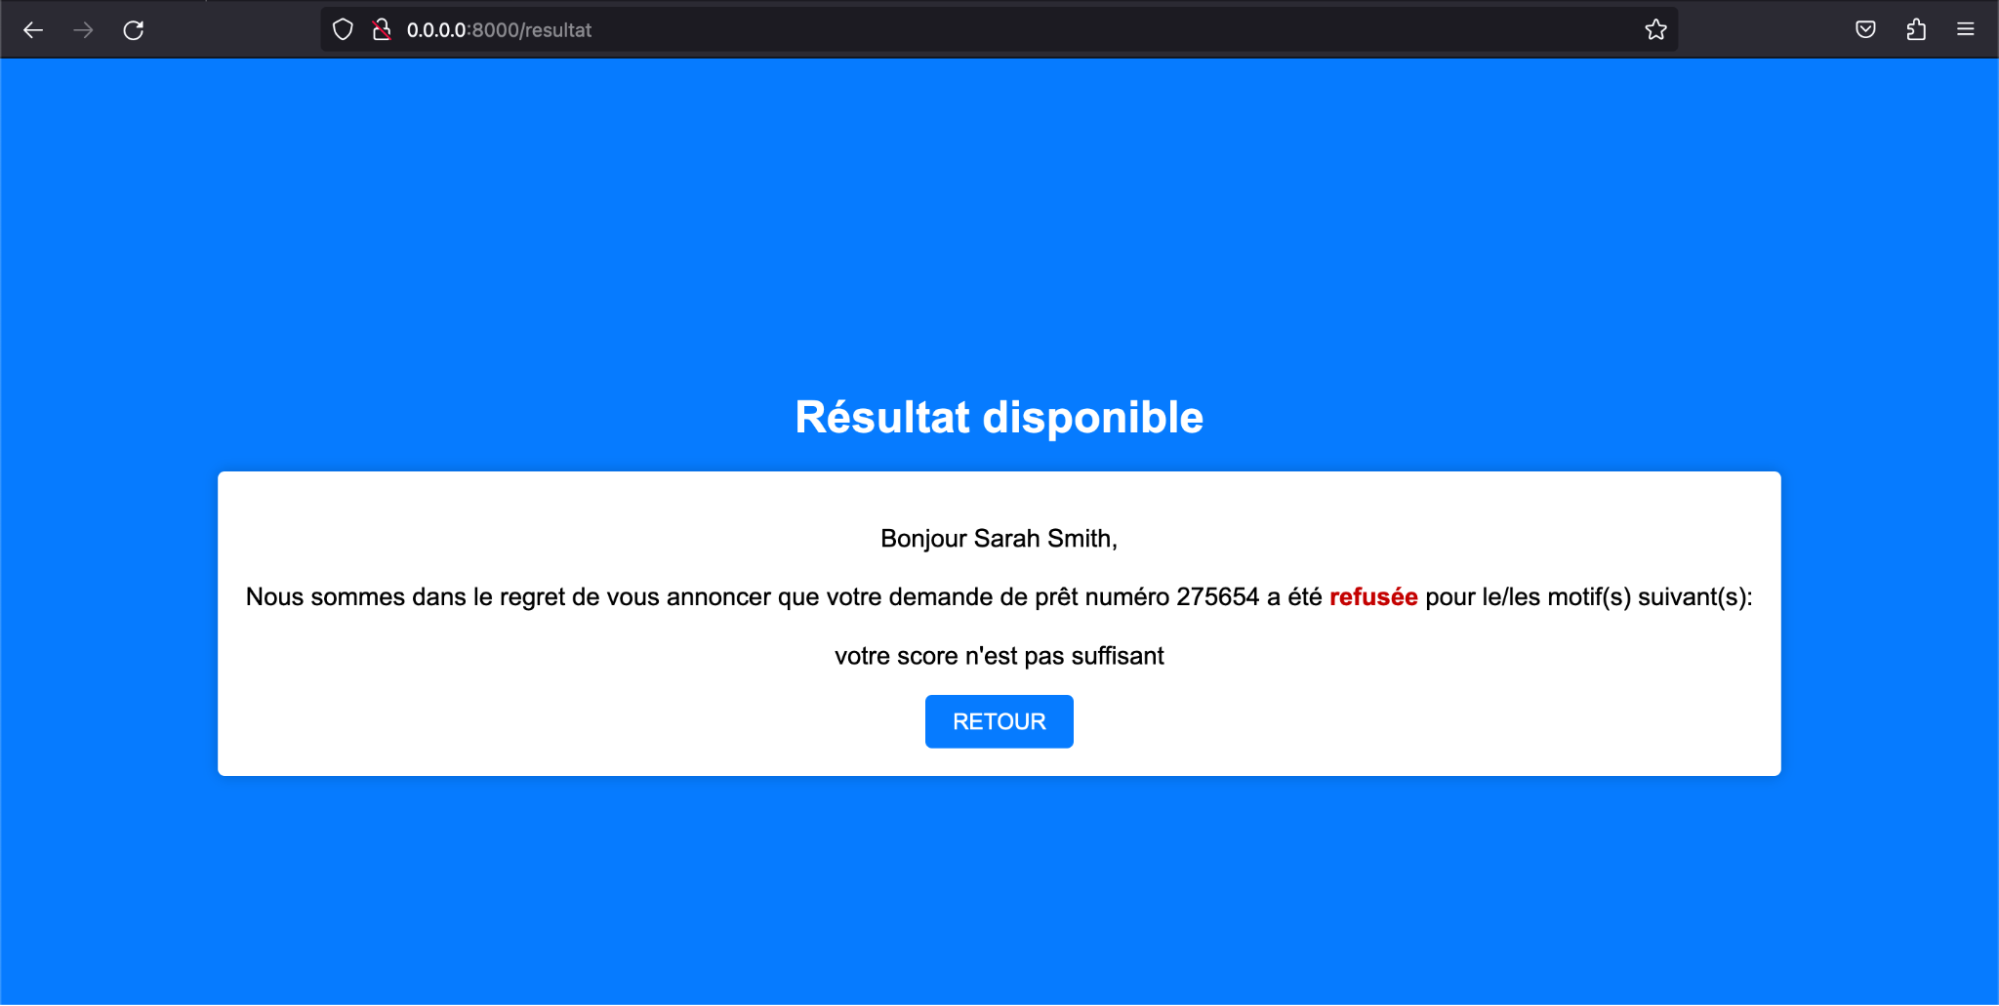
\includegraphics[width=\textwidth]{Images/8.2/confirmationr.png}
     
    \subsubsection{Côté Serveur : Terminal}
    Voici un exemple de ce qui se passe sur le serveur lorsque le client fait sa demande d'évaluation sur l'interface : \\
    \\
    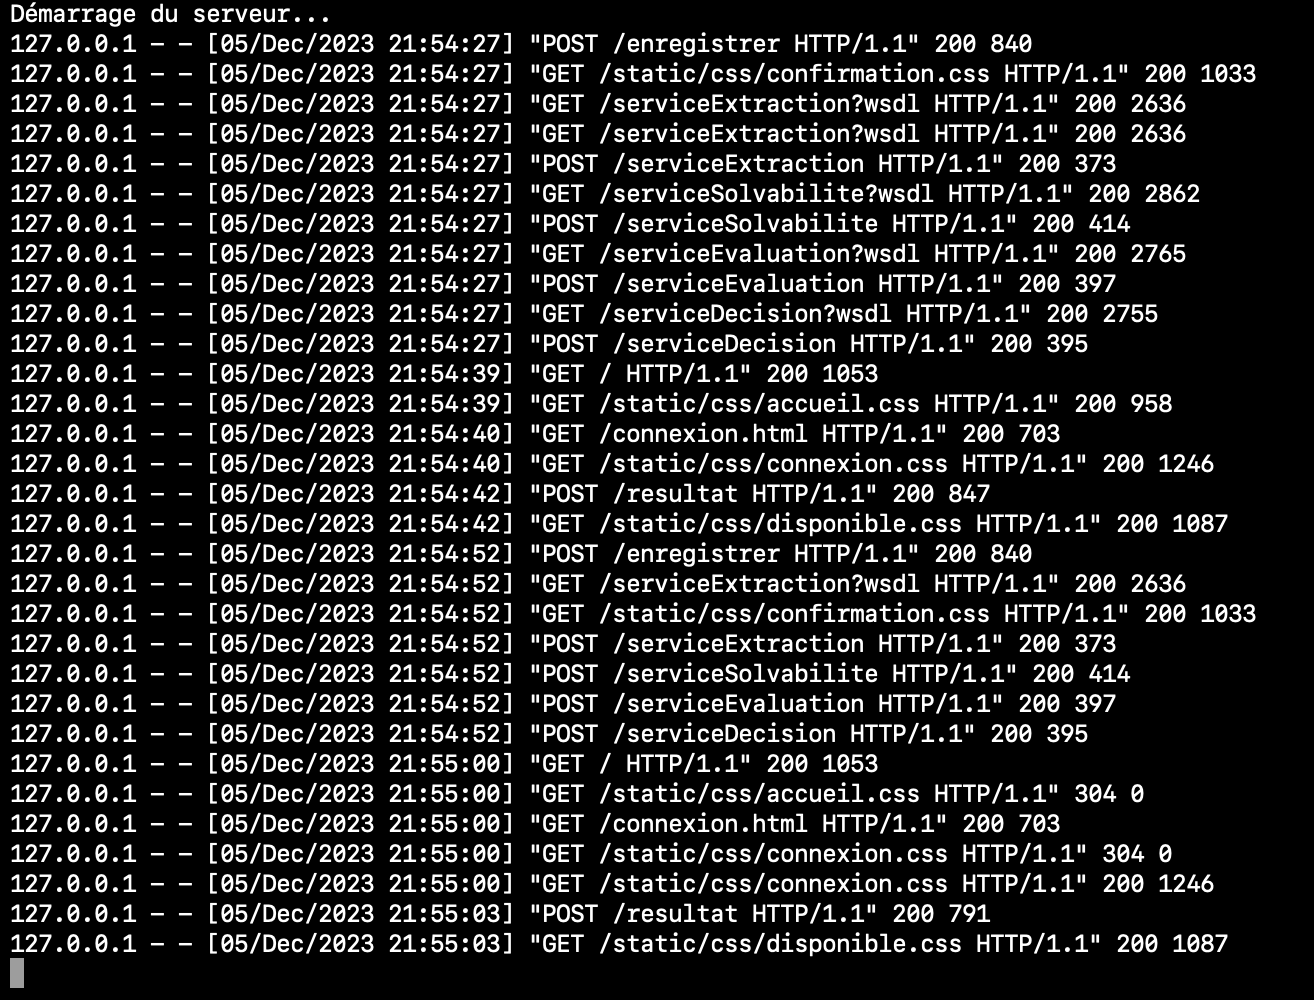
\includegraphics[width=\textwidth]{Images/8.2/serveur.png}

\newpage

    \textbf{Dépôt du formulaire : création du fichier \texttt{.txt} dans \texttt{demandeTxt/}}\\ \\
    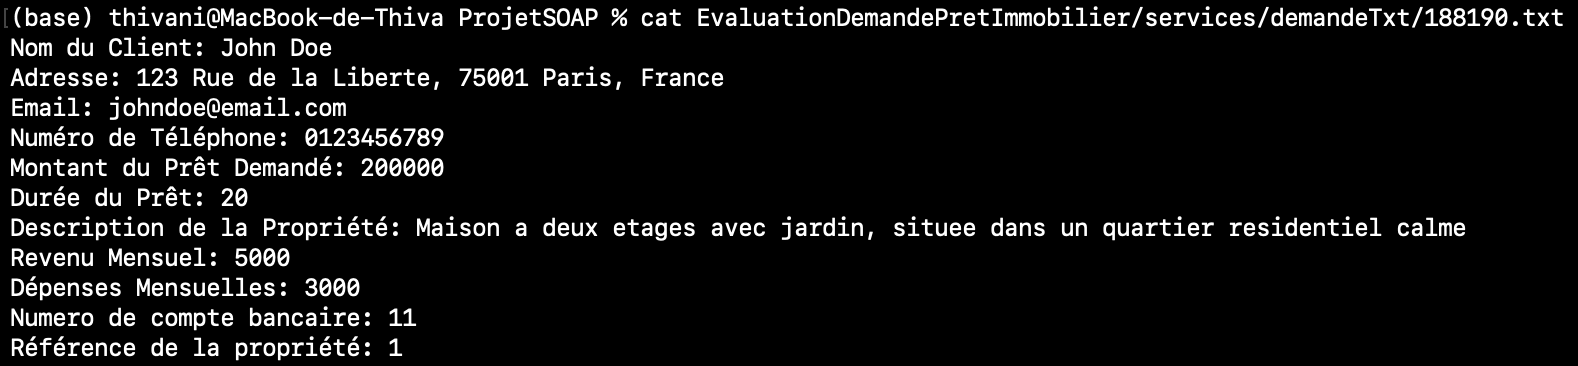
\includegraphics[width=\textwidth]{Images/8.2/demandeTxtP.png}
    \\
    \\
    \textbf{Début de l'évaluation : création du fichier \texttt{.xml} dans \texttt{demandeXml/}}\\ \\
    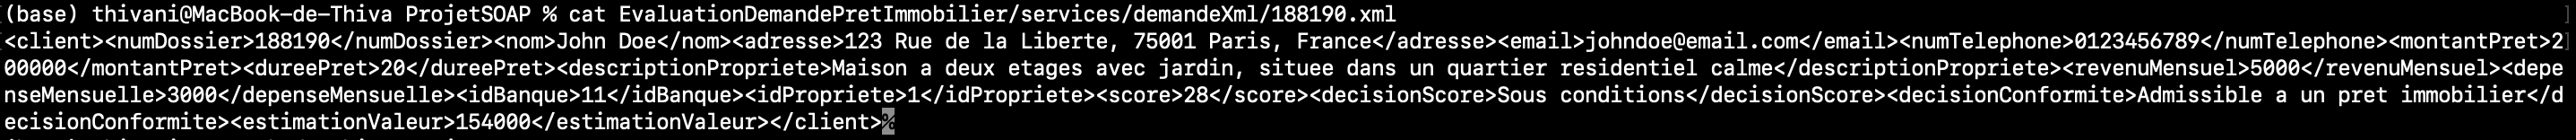
\includegraphics[width=\textwidth]{Images/8.2/demandeXml.png}
    \\
    \\
    \textbf{Fin de l'évaluation : création du fichier \texttt{.txt} dans \texttt{reponseTxt/}}\\ \\
    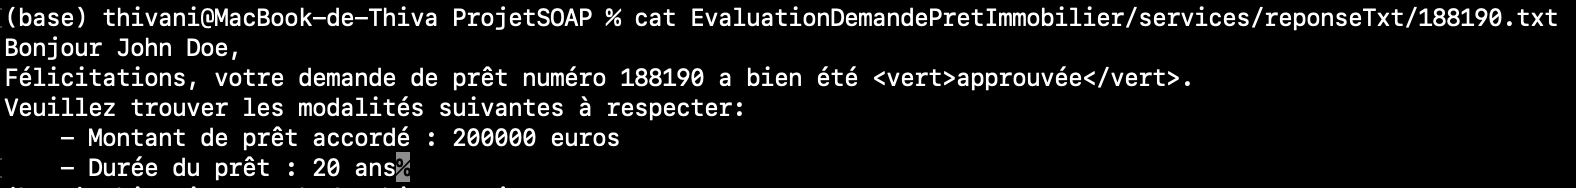
\includegraphics[width=\textwidth]{Images/8.2/reponseTxtP.png}
    \\
    \\
    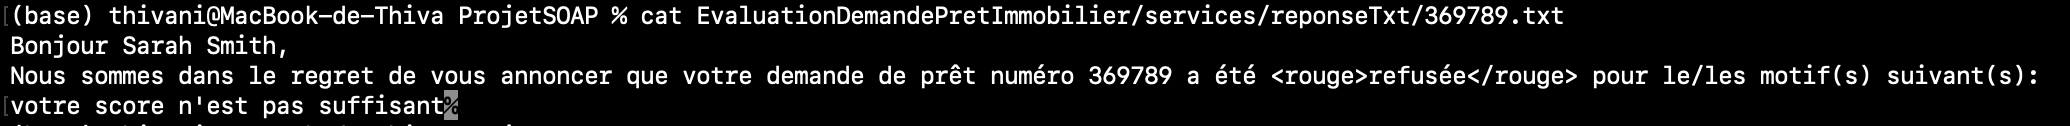
\includegraphics[width=\textwidth]{Images/8.2/reponseTxtN.png}
    \\
    \\
\newpage
\section{Démonstration avec SOAP}
    \subsection{Scénario 1 : Demande de prêt acceptée}
    \subsubsection{Saisie dans le formulaire}
    Voici les informations à saisir pour ce scénario :
    \begin{itemize}
        \item Nom : \texttt{John Doe}
        \item Adresse : \texttt{123 Rue de la Liberte, 75001 Paris, France}
        \item Email : \texttt{johndoe@email.com}
        \item Numéro de téléphone : \texttt{0123456789}
        \item Montant du prêt : \texttt{200000}
        \item Durée du prêt : \texttt{20}
        \item Description de la propriete : \texttt{Maison a deux etages avec jardin, situee dans un quartier residentiel calme}  
        \item Revenus mensuel : \texttt{5000} 
        \item Dépenses mensuelles : \texttt{3000}  
        \item Compte bancaire : \texttt{11}  
        \item Identifiant propriété : \texttt{1}
    \end{itemize}  
    
    \subsubsection{Résultat attendu}
    Voici les résultats attendus pour ce scénario :
    \begin{itemize}
        \item Score : \texttt{28}
        \item Décision Score : \texttt{Sous condition}
        \item Décision Conformité : \texttt{Admissible a un pret immobilier}
        \item Raisons : \texttt{/}
        \item EstimationValeur: \texttt{154000}
    \end{itemize}
    
    \subsubsection{Page résultat attendue}
    Voici la page résultat attendue pour ce scénario: \\
    \\
    \begin{center}
    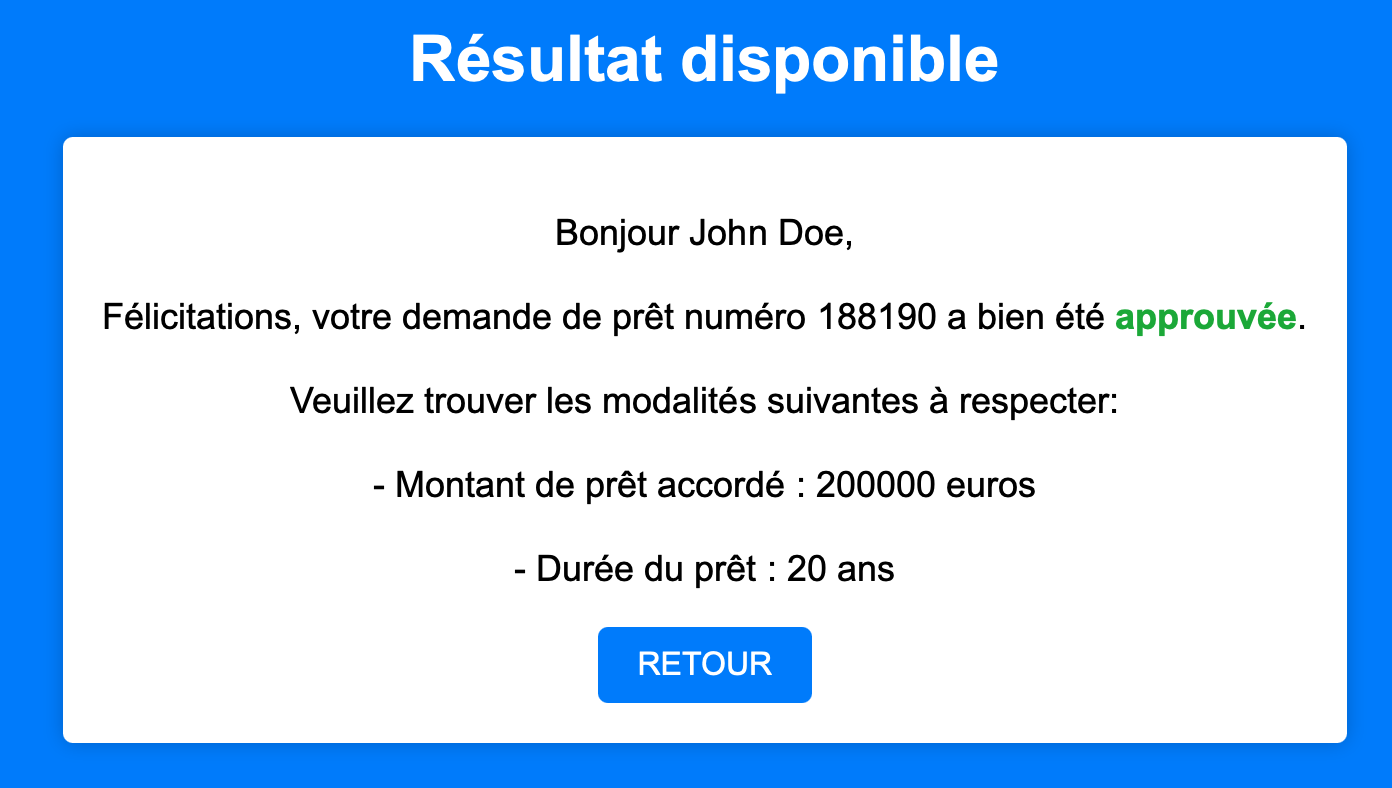
\includegraphics[width=300pt]{Images/9.1/reponsePositive.png}\\
    \end{center}

    \subsection{Scénario 2 : Demande de prêt refusée}
    \subsubsection{Saisie dans le formulaire}
    Voici les informations à saisir pour ce scénario :
    \begin{itemize}
        \item Nom : \texttt{Sarah Smith}
        \item Adresse : \texttt{45 avenue des Etats-Unis, 78000 Versailles, France}
        \item Email : \texttt{sarahsmith@email.com}
        \item Numéro de téléphone : \texttt{0123456788}
        \item Montant du prêt : \texttt{150000}
        \item Durée du prêt : \texttt{30}
        \item Description de la propriété : \texttt{Appartement situee dans un quartier d'affaire} 
        \item Revenus mensuel : \texttt{2000}  
        \item Dépenses mensuelles : \texttt{1500}  
        \item Compte bancaire : \texttt{22}  
        \item Identifiant propriété : \texttt{2}
    \end{itemize}
    
    \subsubsection{Résultat attendu}
    Voici les résultats attendus pour ce scénario :
    \begin{itemize}
        \item Score : \texttt{-1}
        \item Décision Score : \texttt{Non admissible}
        \item Décision Conformité : \texttt{Non admissible a un pret immobilier}
        \item Raisons : \texttt{Normes non reglementaires! Il y a au moins 1 litige en cours}
        \item EstimationValeur: \texttt{0}
    \end{itemize}
    
    
    \subsubsection{Page résultat attendue}
    Voici la page résultat attendue pour ce scénario : \\
    \\
    \begin{center}
    
\includegraphics[width=400pt]{Images/9.2/reponseN.png}\\
    \end{center}
      

\newpage





\section{Modélisation des services sous REST}
    \subsection{Modélisation}
     Voici une architecture à base de service pour mettre en œuvre le processus d’évaluation de demande de prêt immobilier :
    \\
    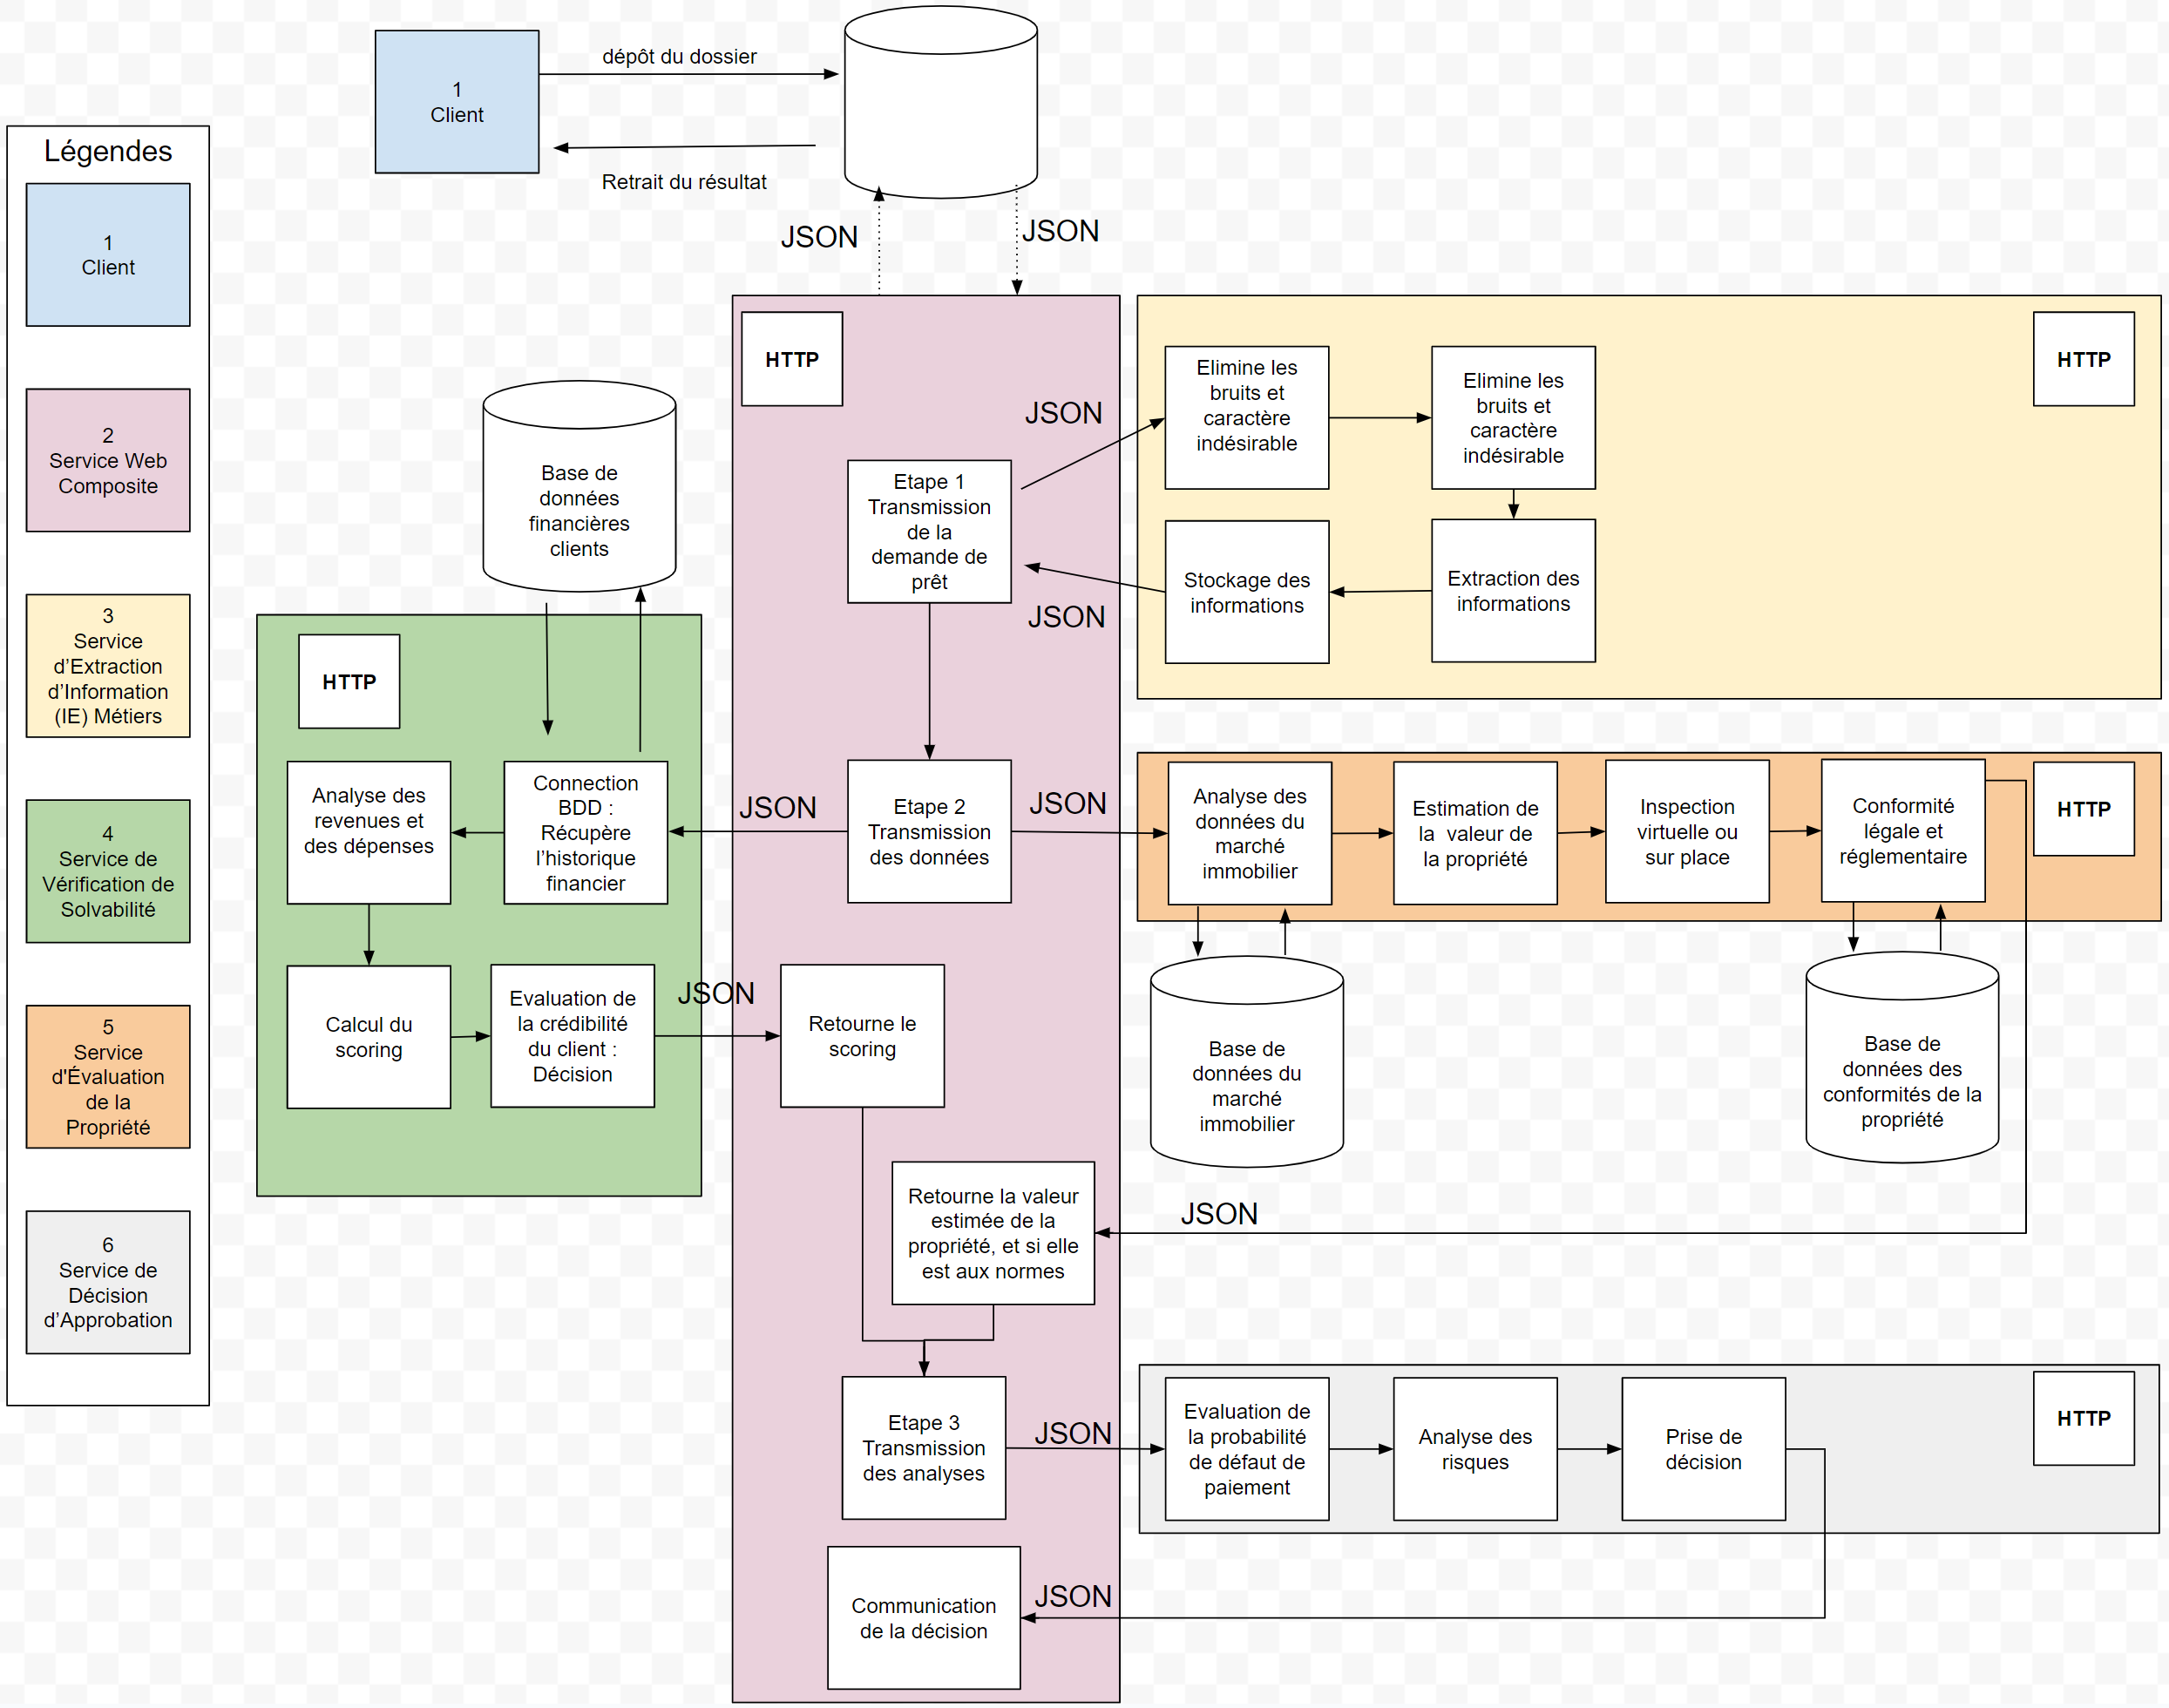
\includegraphics[width=\textwidth]{Images/10.1/modelisation_JSON.png}\\
    \\
    \subsection{Différences par rapport au SOAP}
    Le fonctionnement interne des services se déroule de la même manière que le SOAP à quelques différences près. Voici les éléments qui changent par rapport à la partie sur le SOAP :
    \begin{itemize}
        \item les bases de données Banque, Immobilier, marcheImmobilier changent de format : les fichiers \texttt{JSON} disparaissent et deviennent des BDD SQLite \texttt{banque.db, immobilier.db et marcheImmobilier.db};
        \item les fichiers \texttt{XML} et \texttt{txt} disparaissent et deviennent des tables dans la BDD \texttt{evaluationPret.db};
        \item apparition d'un fichier App.py qui contient toutes les routes y compris celles pour communiquer entre les différents services;
        \item les requêtes faisant appel au fichier WSDL des services n'existent plus;
        \item les requêtes SOAP disparaissent et laissent place aux requêtes REST à l'aide du module \texttt{requests};
        \item les messages sont envoyés sous format \texttt{JSON} au lieu du \texttt{XML} entre les services.
    \end{itemize}

    
\section{Implémentation avec REST}
	\subsection{Structure du projet}
    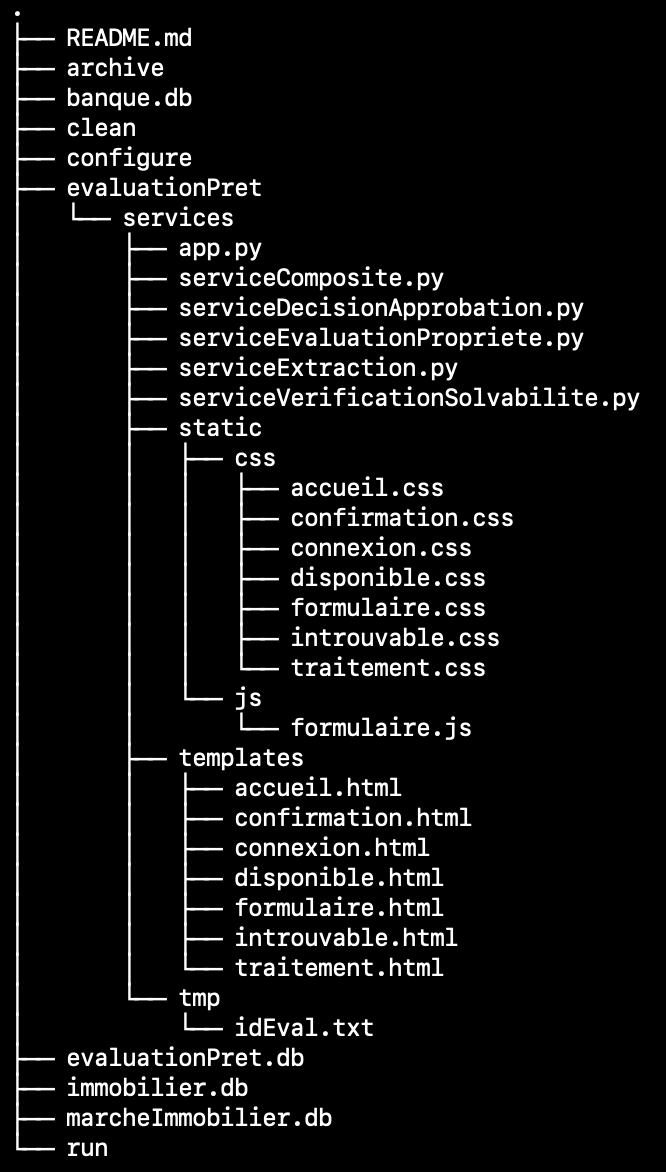
\includegraphics[width=225pt]{Images/11.1/tree.png}\\
    
    \begin{itemize}
    
        \item Dans le dossier ProjetREST, nous avons:
        \begin{itemize}
            \item un dossier \texttt{evaluationPret}, contenant le coeur du projet;
            \item un \texttt{README.md}, donnant les commandes et les scénarios à exécuter;
            \item des scripts (\texttt{archive, clean, configure, run});
            \item et les fichiers \texttt{.db} contenant les bases de données SQLite : evaluationPret, banque, immobilier, marcheImmobilier.
        \end{itemize}
    
        \item Dans le dossier \texttt{evaluationPret},  nous avons un dossier \texttt{services} contenant le coeur du projet. 
        
        \item Le projet se situant dans le dossier \texttt{services}, il est composé de:
        \begin{itemize}
            \item le fichier \texttt{app.py} qui contient toutes les routes entre les services;
            \item les fichiers \texttt{.py} pour chaque service tels que : \texttt{serviceComposite.py, serviceDecisionApprobation.py, serviceEvaluationPropriete.py, serviceExtraction.py, serviceVerificationSolvabilite.py};
          \item un dossier \texttt{static} qui contient l'ensemble des fichiers \texttt{CSS} et \texttt{JS} nécessaire pour l'interface web;
          \item un dossier \texttt{templates} qui contient l'ensemble des fichiers \texttt{HTML} contenant les pages web de l'interface;
          \item ainsi qu'un dossier \texttt{tmp} qui contient des fichiers temporaires qui sont utilisés lors de l'évaluation tel que \texttt{idEval.txt}
        \end{itemize}

    \end{itemize}

    
    \subsection{Spécifications des services}
    
        \subsubsection{Service Composite}
            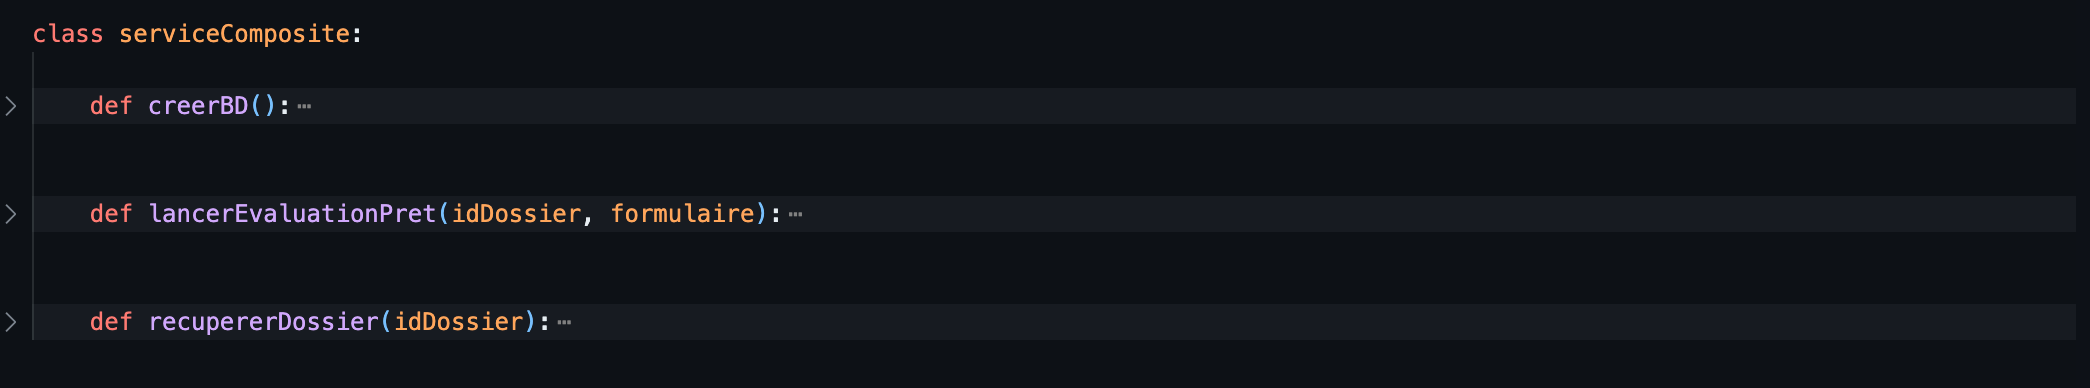
\includegraphics[width=\textwidth]{Images/11.2/composite.png} \\ \\ 
            Le \texttt{service Composite} est l'orchestrateur de ce projet. Il permet de lancer l'évaluation de la demande de prêt et de faire appel aux autres services (Extraction, VerificationSolvabilité, EvaluationPropriété, Décision). Il contient les fonctions suivantes:
            
            \begin{itemize}
            \item \texttt{creerBD} : permet de créer la BD \texttt{EvaluationPret} avec les tables \texttt{DEMANDE, EVALUATION, RESULTAT} afin de stocker les données utiles lors de l'évaluation de la demande de prêt;
            \item \texttt{lancerEvaluationPret} : permet de lancer l'évaluation de prêt et de communiquer avec les autres services;
            \item \texttt{recupererDossier} : permet de récupérer le formulaire stocké dans la base de données \texttt{evaluationPret.db} avec l'\texttt{idDossier} mentionné.
            \end{itemize}


        \subsubsection{Service Extraction}
            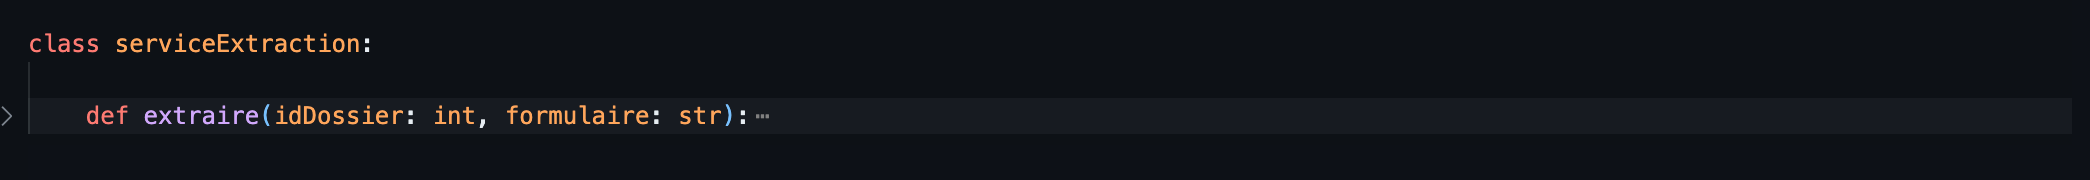
\includegraphics[width=\textwidth]{Images/11.2/extraction.png} \\ \\ 
            Le \texttt{service Extraction} contient une fonction principale \texttt{extraire} qui permet de récupérer le formulaire pour un idDossier donné, de l'extraire en entités et de créer un nouveau tuple dans la table EVALUATION.

            
        \subsubsection{Service VerificationSolvabilite}
            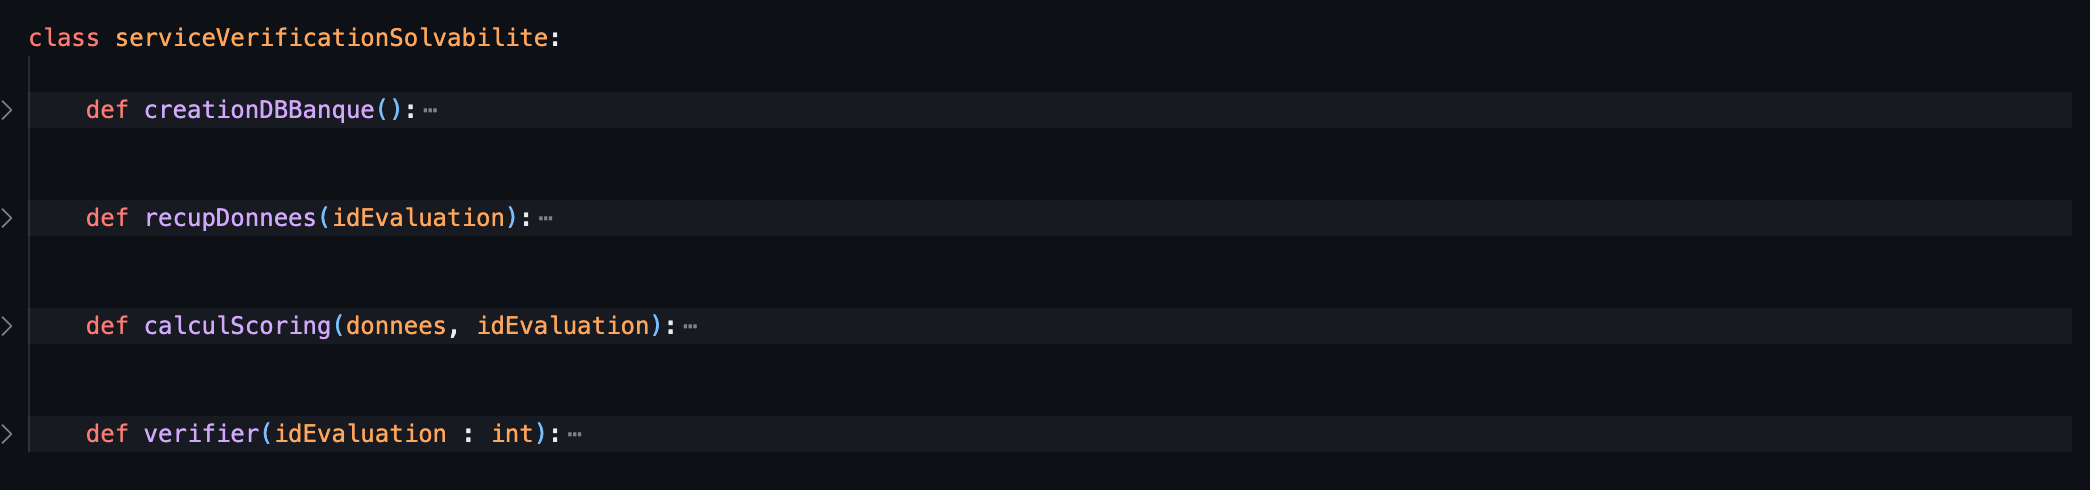
\includegraphics[width=\textwidth]{Images/11.2/solvabilite.png} \\ \\ 
             Le \texttt{service VerificationSolvabilité} permet de vérifier la solvabilité en fonction de la situation financière du demandeur de prêt. Pour cela, il va recueillir les données nécessaires du client et calculer le scoring avec ces données. Il contient les fonctions suivantes:
             
            \begin{itemize}
            \item \texttt{creationDBBanque} : permet de créer la base de données \texttt{Banque} avec une table \texttt{BANQUE} afin d'avoir la situation financière des clients;
            \item \texttt{recupDonnees} : permet de récupérer les données concernant le client et sa situation financière provenant de la base de données \texttt{Banque};
            \item \texttt{calculScoring} : permet de calculer le scoring du client en fonction des données récupérées dans la fonction précédente et d'écrire le score ainsi que la décision du score dans la table \texttt{EVALUATION};
            \item \texttt{verifier} : fonction principale qui permet d'appliquer les 3 fonctions précédentes.
            \end{itemize}

        \subsubsection{Service EvaluationPropriete}
            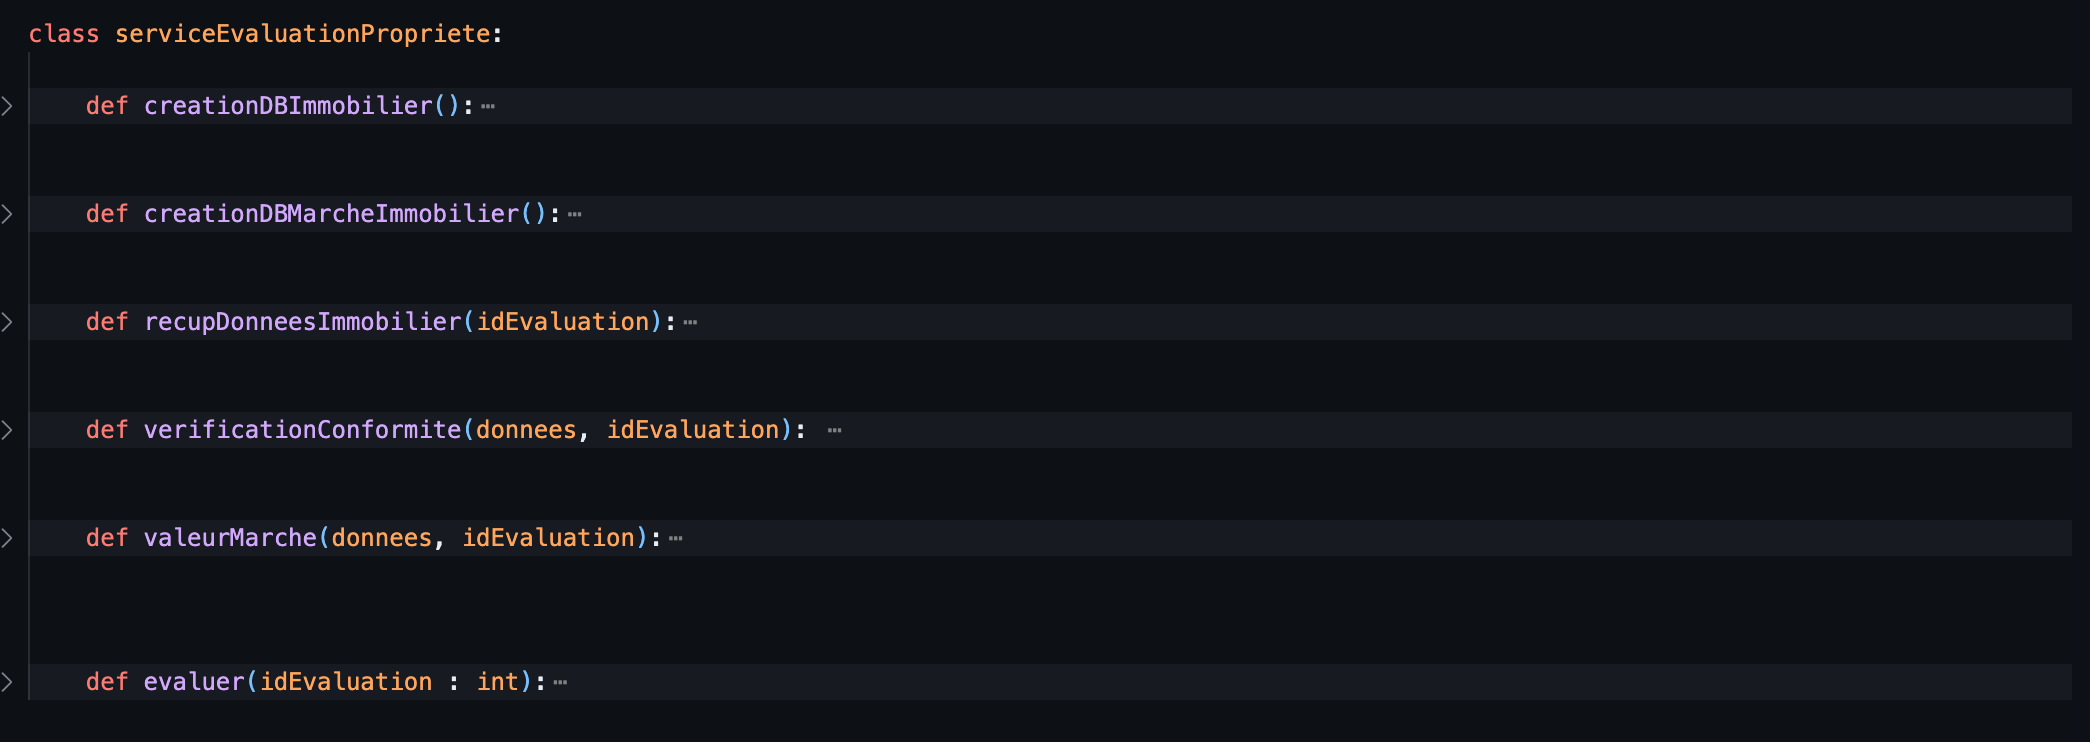
\includegraphics[width=\textwidth]{Images/11.2/evaluation.png} \\ \\ 
            Le \texttt{serviceEvaluationPropriete} permet d'évaluer la propriété pour laquelle le client demande son prêt. Pour cela, il va dans un premier temps vérifier la conformité de la propriété et ensuite vérifier la valeur de cette propriété dans le marché. Il contient les fonctions suivantes:
            
            \begin{itemize}
            \item \texttt{creationDBImmobilier} : permet de créer la base de données \texttt{Immobilier} avec une table \texttt{IMMOBILIER} afin d'avoir plus d'informations sur la propriété;
            \item \texttt{creationDBMarcheImmobilier} : permet de créer la base de données \texttt{MarcheImmobilier} avec une table \texttt{MARCHEIMMOBILIER} afin d'avoir des informations sur les propriétés similaires situées dans la même ville que celle évaluée;
            \item \texttt{recupDonneesImmobilier} : permet de récupérer les données concernant les informations de la propriété provenant de la base de données \texttt{IMMOBILIER}; 
            \item \texttt{verificationConformite} : permet de vérifier si la situation de la propriété est conforme et légale grâce aux données récupérées dans la fonction précédente et d'écrire la décision de conformité dans la table \texttt{EVALUATION};
            \item \texttt{valeurMarche} : permet de calculer la moyenne des valeurs des propriétés similaires situées dans la même ville en récupérant les données nécessaires dans la base de données \texttt{MARCHEIMMOBILIER} et d'écrire l'estimation valeur dans la table \texttt{EVALUATION};
            \item \texttt{evaluer} : fonction principale qui permet d'appliquer les 5 fonctions précédentes.
            \end{itemize}
            
        \subsubsection{Service DecisionApprobation}
            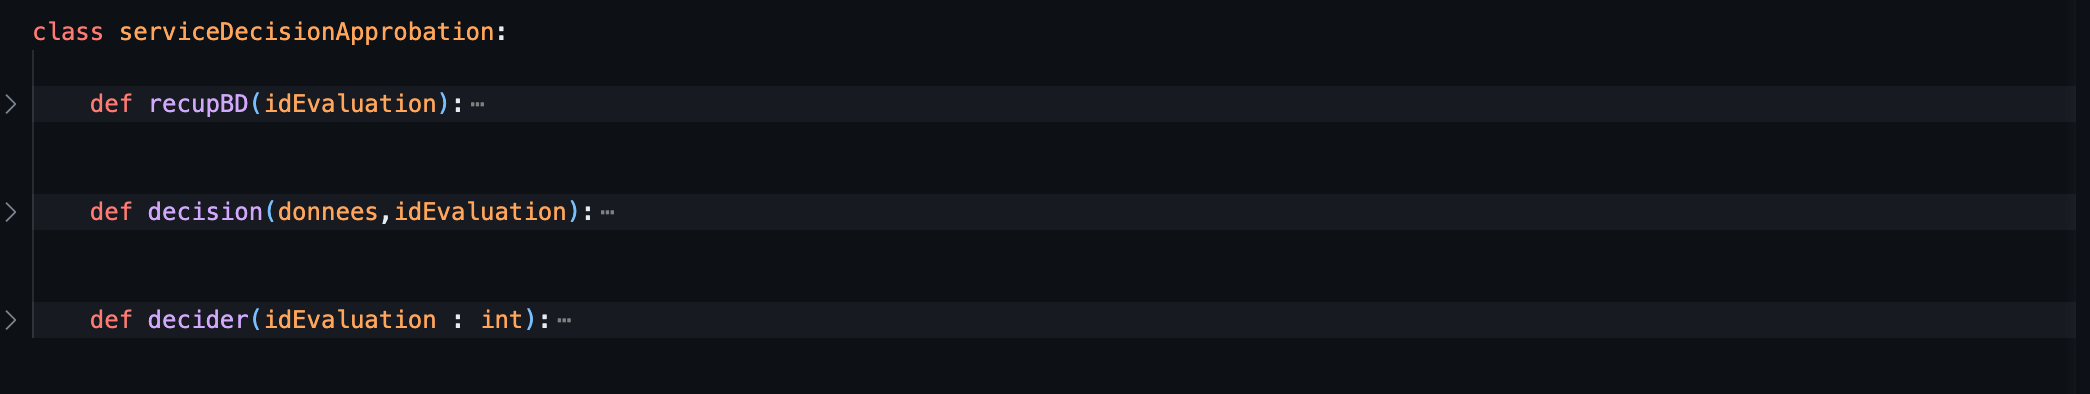
\includegraphics[width=\textwidth]{Images/11.2/decision.png} \\ \\ 
            Le \texttt{serviceDecisionApprobation} permet de générer une décision suite à l'évaluation du prêt effectué par le \texttt{serviceVerificationSolvabilité} et le \texttt{serviceEvaluationPropriete}. Il contient les fonctions suivantes:
            \begin{itemize}
            \item \texttt{recupBD} : permet de récupérer les données nécessaires pour pouvoir générer une décision dans la table \texttt{EVALUATION};
            \item \texttt{decision} : permet de générer un résultat suite aux évaluations des services précédentes. On crée un tuple dans la table \texttt{RESULTAT} qui sera récupéré par le \texttt{service Composite} pour pouvoir l'afficher sur l'interface lorsque le client lui demande les résultats.
            \item \texttt{decider} : fonction principale qui permet d'appliquer les 2 fonctions précédentes.
            \end{itemize}
        
        \subsubsection{App}
            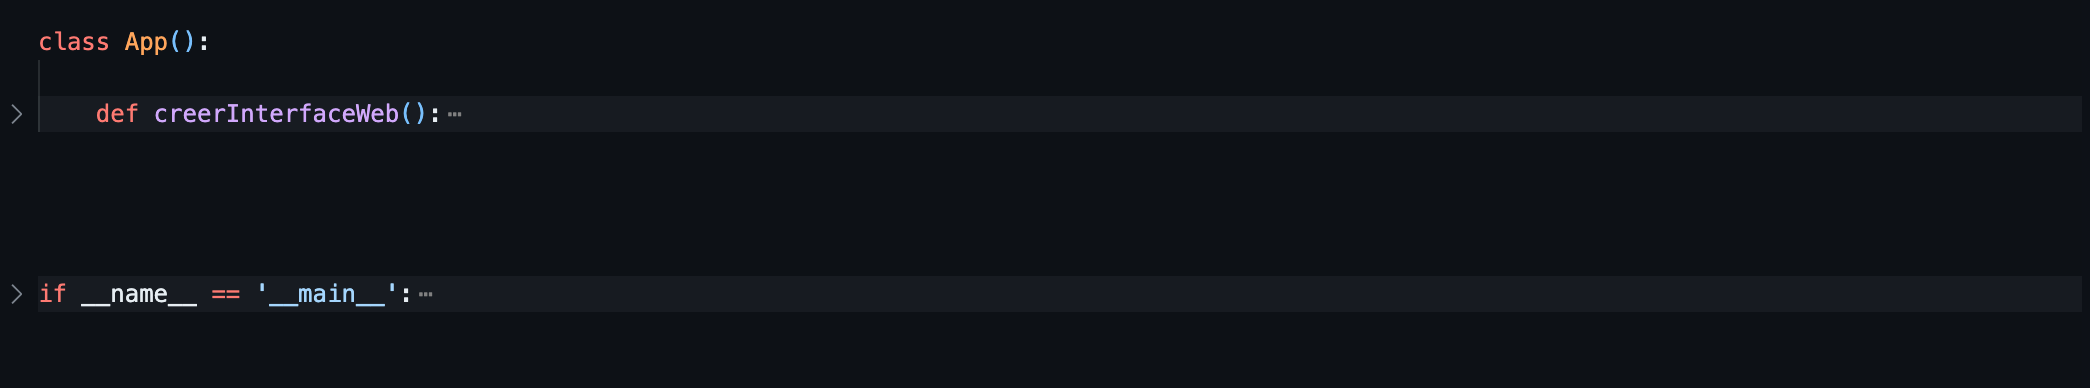
\includegraphics[width=\textwidth]{Images/11.2/app.png} \\ \\ 
            Le fichier \texttt{App.py} regroupe toutes les routes de ce projet: les routes pour chaque page web, les routes pour enregistrer le formulaire ainsi que pour afficher le résultat, ainsi que les routes permettant de communiquer entre 2 services sous l'API REST. 


        
	\subsection{Interaction entre les services sous l'API REST}
    \begin{itemize}
        \item \textbf{Service Composite $\leftrightarrow$ Service Extraction} \\
        \\
        \textbf{Request POST afin d'envoyer l'idDossier et le formulaire au service Extraction}\\
        \\
        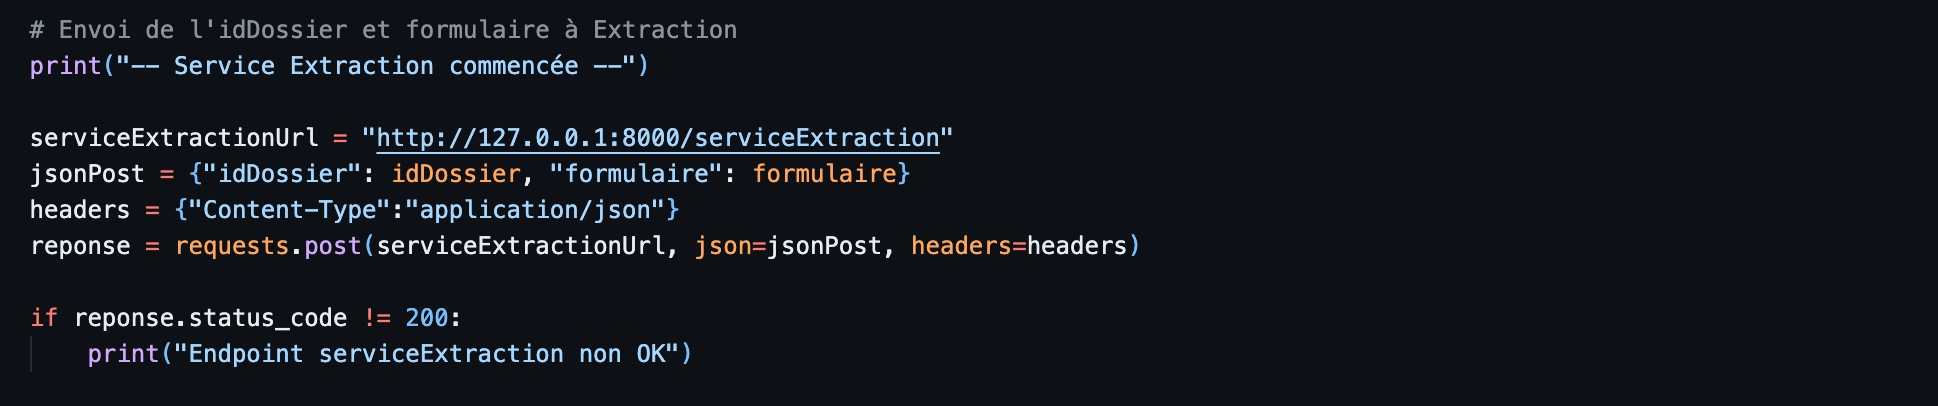
\includegraphics[width=\textwidth]{Images/11.3/requeteExtraction.png}\\
        \\
        \textbf{Route permettant d'appeler la fonction principale du service Extraction avec idDossier et formulaire récupéré du service Composite}\\
        \\
        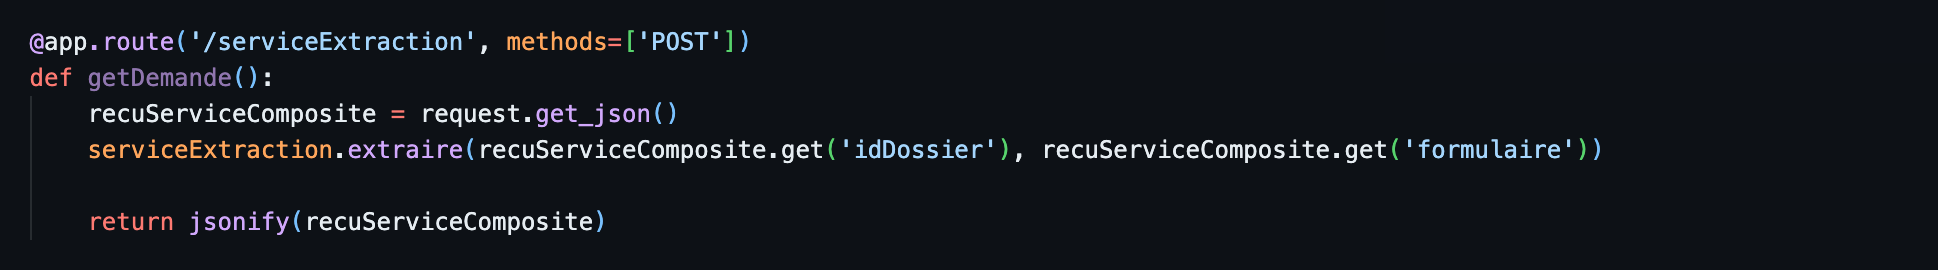
\includegraphics[width=\textwidth]{Images/11.3/routeExtraction.png}\\
        \\
        \textbf{Request GET afin de recevoir l'idEvaluation du service Extraction}\\
        \\
        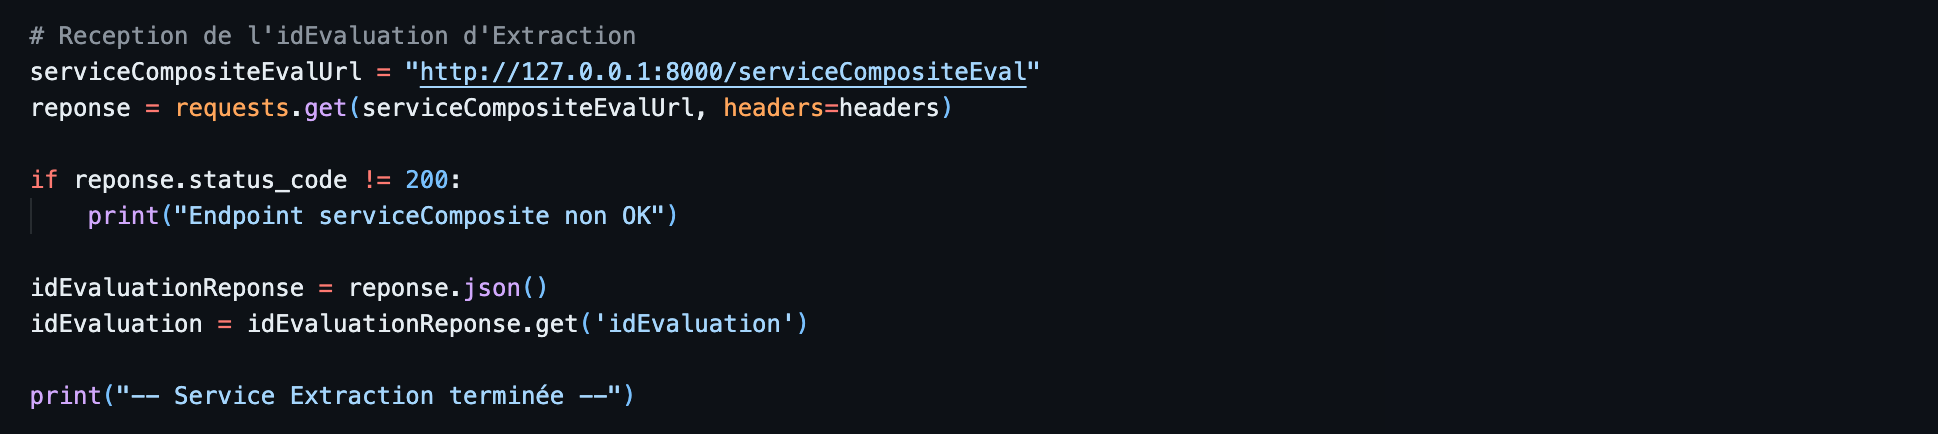
\includegraphics[width=\textwidth]{Images/11.3/requeteExtraction2.png}\\
        \\
        
        \newpage
        
        \textbf{Route permettant la communication entre les services Composite et Extraction pour l'idEvaluation}\\
        \\
        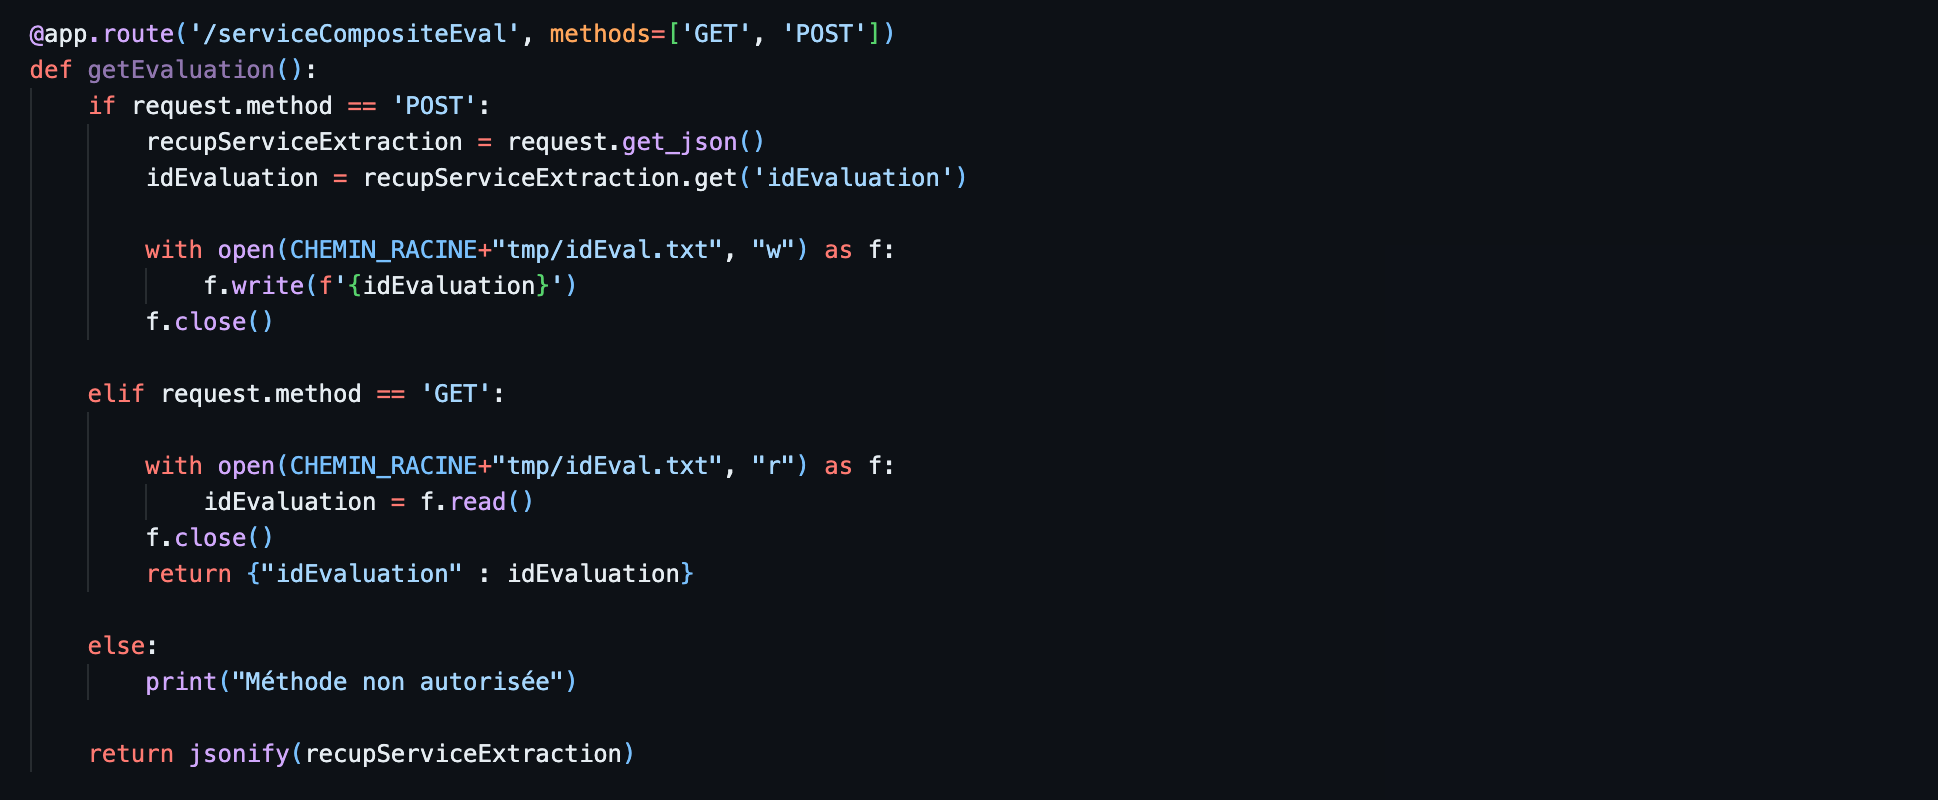
\includegraphics[width=\textwidth]{Images/11.3/routeComposite.png}\\
        \item \textbf{Service Composite $\leftrightarrow$ Service VerificationSolvabilité} \\
        \\
        \textbf{Request POST afin d'envoyer l'idEvaluation au service VerificationSolvabilite}\\
        \\
        \includegraphics[width=\textwidth]{Images/11.3/requeteSolvabilite.png}\\
        \\
        \textbf{Route permettant d'appeler la fonction principale du service VerificationSolvabilite avec idEvaluation récupéré du service Composite}\\
        \\
        \includegraphics[width=\textwidth]{Images/11.3/routeSolvabilite.png}\\
        \item \textbf{Service Composite $\leftrightarrow$ Service EvaluationPropriete} \\
        \\
        \textbf{Request POST afin d'envoyer l'idEvaluation au service EvaluationPropriete}\\
        \\
        \includegraphics[width=\textwidth]{Images/11.3/requeteEvaluation.png}\\
        \\
        
        \newpage
        
        \textbf{Route permettant d'appeler la fonction principale du service EvaluationPropriete avec idEvaluation récupéré du service Composite}
        \\
        \includegraphics[width=\textwidth]{Images/11.3/routeEvaluation.png}\\
        \item \textbf{Service Composite $\leftrightarrow$ Service DecisionApprobation} \\
        \\
        \textbf{Request POST afin d'envoyer l'idEvaluation au service DecisionApprobation}
        \\
        \includegraphics[width=\textwidth]{Images/11.3/requeteDecision.png}\\
        \\
        \textbf{Route permettant d'appeler la fonction principale du service DecisionApprobation avec idEvaluation récupéré du service Composite}
        \\
        \includegraphics[width=\textwidth]{Images/11.3/routeDecision.png}\\
        \\
          
    \end{itemize}
    
 \newpage
    
 \section{Démonstration avec REST}
 
    \subsection{Scénario 1 : Profil parfait}
        \subsubsection{Saisie dans le formulaire}
        Voici les informations à saisir pour ce scénario :
        \begin{itemize}
            \item Nom : \texttt{Paul Gauthier}
            \item Adresse : \texttt{12 Rue du Pont Neuf, 91120 Palaiseau, France}  
            \item Email : \texttt{paul.gauthier@email.com}  
            \item Numéro de téléphone : \texttt{01 12 23 34 45}  
            \item Montant du pret : \texttt{160000}  
            \item Duree du pret : \texttt{10}  
            \item Description de la propriete : \texttt{Appartement a 6 etages avec un petit balcon}  
            \item Revenus mensuel : \texttt{12000}
            \item Depenses mensuelles : \texttt{2000}
            \item Compte bancaire : \texttt{33}
            \item Identifiant propriété : \texttt{3}
        \end{itemize}
        
        \subsubsection{Résultat attendu}
        Voici les résultats attendus pour ce scénario :
        \begin{itemize}
            \item Score : \texttt{32}
            \item Décision Score : \texttt{Très favorable}
            \item Décision Conformité : \texttt{Admissible a un pret immobilier}
            \item Raisons : \texttt{/}
            \item EstimationValeur: \texttt{148000}
        \end{itemize}
        
        \subsubsection{Page résultat attendu}
        Voici la page résultat attendue pour ce scénario: \\
        \\
        \begin{center}
            \includegraphics[width=300pt]{Images/12.1/resultat1.png}\\
        \end{center}
        
 \newpage
 
    \subsection{Scénario 2 : Profil emploi instable}
        \subsubsection{Saisie dans le formulaire}
        Voici les informations à saisir pour ce scénario :
        \begin{itemize}
            \item Nom : \texttt{Jack Daniel}
            \item Adresse : \texttt{52 Avenue de la gare, 91120 Palaiseau, France}  
            \item Email : \texttt{jack.daniel@email.com}  
            \item Numéro de téléphone : \texttt{01 12 23 34 46}  
            \item Montant du pret : \texttt{130000}  
            \item Duree du pret : \texttt{15}  
            \item Description de la propriete : \texttt{Appartement de 5 etages}  
            \item Revenus mensuel : \texttt{7000}
            \item Depenses mensuelles : \texttt{3000}
            \item Compte bancaire : \texttt{44}
            \item Identifiant propriété : \texttt{4}
        \end{itemize}
        
        \subsubsection{Résultat attendu}
        Voici les résultats attendus pour ce scénario :
        \begin{itemize}
            \item Score : \texttt{27}
            \item Décision Score : \texttt{Sous condition}
            \item Décision Conformité : \texttt{Admissible a un pret immobilier}
            \item Raisons : \texttt{/}
            \item EstimationValeur: \texttt{135000}
        \end{itemize}
        
        \subsubsection{Page résultat attendu}
        Voici la page résultat attendue pour ce scénario: \\
        \\
        \begin{center}
            \includegraphics[width=300pt]{Images/12.2/resultat2.png}\\
        \end{center}

  \newpage
  
    \subsection{Scénario 3 : Profil score trop faible}
        \subsubsection{Saisie dans le formulaire}
        Voici les informations à saisir pour ce scénario :
        \begin{itemize}
            \item Nom : \texttt{Victor Wolf}
            \item Adresse : \texttt{39 Rue Geais Padidee, 91120 Palaiseau, France}  
            \item Email : \texttt{victor.wolf@email.com}  
            \item Numéro de téléphone : \texttt{01 12 23 34 47}  
            \item Montant du pret : \texttt{70000}  
            \item Duree du pret : \texttt{25}  
            \item Description de la propriete : \texttt{Maison avec deux etages et un grand jardin}  
            \item Revenus mensuel : \texttt{10000}
            \item Depenses mensuelles : \texttt{6000}
            \item Compte bancaire : \texttt{55}
            \item Identifiant propriété : \texttt{5}
        \end{itemize}
        
        \subsubsection{Résultat attendu}
                Voici les résultats attendus pour ce scénario :
        \begin{itemize}
            \item Score : \texttt{12}
            \item Décision Score : \texttt{Non Admissible}
            \item Décision Conformité : \texttt{Admissible a un pret immobilier}
            \item Raisons : \texttt{Score pas suffisant}
            \item EstimationValeur: \texttt{200000}
        \end{itemize}
        
        \subsubsection{Page résultat attendu}
        Voici la page résultat attendue pour ce scénario: \\
        \\
        \begin{center}
            \includegraphics[width=400pt]{Images/12.3/resultat3.png}\\
        \end{center}

\newpage

    \subsection{Affichage côté Serveur}
    \subsubsection{Scénario 1 : Profil parfait}
    \includegraphics[width=400pt]{Images/12.4/serveur1.png}
    \subsubsection{Scénario 2 : Profil emploi instable}
    \includegraphics[width=400pt]{Images/12.4/serveur2.png}\\
    
    \newpage
    
    \subsubsection{Scénario 3 : Profil score trop faible}
    \includegraphics[width=400pt]{Images/12.4/serveur3.png}

    \subsection{Bases de données evaluationPret.db}
    \subsubsection{Table DEMANDE : formulaires saisis par les 3 clients des scénarios précédents}
    \includegraphics[width=400pt]{Images/12.5/demandeSQL.png}
    
    \subsubsection{Table EVALUATION : fin de l'évaluation des prêts pour les 3 clients}
    \includegraphics[width=400pt]{Images/12.5/evaluationSQL.png}
    
    \subsubsection{Table RESULTAT : résultats des 3 clients}
    \includegraphics[width=400pt]{Images/12.5/resultatSQL.png}


\end{document}